\chapter{An\'alisis}
\section{Catálogo de Requisitos}
En esta sección se definirán los distintos requisitos que se contemplan para el sistema. Eso incluye los requisitos funcionales, los no funcionales y los de información.

\subsection{Requisitos Funcionales}
\label{lrf} Los requerimientos funcionales (RF) de un sistema sirven para especificar lo que este debe poder realizar, de modo que son aquellos que describen su comportamiento cuando se cumplen ciertas condiciones.

\addtocounter{tabla}{1}
El primer requisito funcional, que podemos observar en la \textbf{\hyperref[tab:rfIniSes]{Tabla \arabic{tabla}}}, requiere al sistema que cualquier Colegiado o Responsable tenga la posibilidad de iniciar sesión con su cuenta de usuario, usando su número de colegiado y su contraseña. Esto será necesario para poder realizar cualquier otra actividad propia de los roles de Colegiado o de Responsables.

\begin{table}[!htbp]
  \centering
  \addtocounter{rf}{1}
  \begin{tabular}{|r | p{98mm}|}
    RF-\arabic{rf}  & Iniciar Sesión \\ \hline
    Descripción & El sistema debe permitir a los Colegiados iniciar sesión con su número de colegiado y contraseña.
    \\ \hline
  \end{tabular}
  \caption{Requisito Funcional \arabic{rf} - Iniciar Sesión}
  \label{tab:rfIniSes}
\end{table}
\FloatBarrier

\addtocounter{tabla}{1}
El segundo requisito (\textbf{\hyperref[tab:rfGestColeg]{Tabla \arabic{tabla}}}) define la gestión de los colegiados registrados en el sistema. Este contempla las actividades de dar de alta, modificación y consulta de los mismos. Se ha obviado la posibilidad de eliminar los colegiados del sistema para evitar la inconsistencia de los datos.

\begin{table}[!htbp]
  \centering \addtocounter{rf}{1}
  \begin{tabular}{|r | p{98mm}|}
    RF-\arabic{rf}  & Gestión de Colegiados \\ \hline
    Descripción & El sistema debe permitir a los Colegiados:
    \begin{itemize}
	  \item Consultar su información personal.
    \end{itemize}
    Los Responsables deben poder:
    \begin{itemize}
	  \item Dar de alta en el TAP a colegiados.
	  \item Consultar la información de los colegiados.
	  \item Actualizar la información de los colegiados.
    \end{itemize}
    \\ \hline
  \end{tabular}
  \caption{Requisito Funcional \arabic{rf} - Gestión de Colegiados}
  \label{tab:rfGestColeg}
\end{table}
\FloatBarrier

\addtocounter{tabla}{1}
Tras la gestión de colegiados, se define un requisito para la gestión de los tipos de lista considerados por el Colegio para los TAP (\textbf{\hyperref[tab:rfGestTipoLst]{Tabla \arabic{tabla}}}). Con ello se permite crear, modificar o consultar los tipos de listas del sistema.

\begin{table}[!htbp]
  \centering \addtocounter{rf}{1}  
  \begin{tabular}{|r | p{98mm}|}
    RF-\arabic{rf}  & Gestión de Tipos de Lista \\ \hline
    Descripción &  El sistema debe permitir a los Usuarios:
    \begin{itemize}
	  \item Consultar los tipos de lista.
    \end{itemize}
    Los Responsables deben poder:
    \begin{itemize}
	  \item Crear nuevos tipos de lista.
	  \item Actualizar la información de los tipos de lista.
    \end{itemize}
    \\ \hline
  \end{tabular}
  \caption{Requisito Funcional \arabic{rf} - Gestión de Tipos de Lista}
  \label{tab:rfGestTipoLst}
\end{table}
\FloatBarrier

\addtocounter{tabla}{1}
También se contará con la gestión de campos de especialización (\textbf{\hyperref[tab:rfGestEspec]{Tabla \arabic{tabla}}}), que servirán para establecer los requisitos para pertenecer a las listas y para definir las habilidades con las que cuentan los colegiados. Con ello se permite crear, modificar o consultar campos de especialización, además de asignarlas a colegiados o requerirlas en las listas.

\begin{table}[!htbp]
  \centering \addtocounter{rf}{1}  
  \begin{tabular}{|r | p{98mm}|}
    RF-\arabic{rf}  & Gestión de Campos de Especialización \\ \hline
    Descripción &  El sistema debe permitir a los Colegiados:
    \begin{itemize}
	  \item Consultar sus especializaciones.
    \end{itemize}
    Los Responsables deben poder:
    \begin{itemize}
	  \item Crear nuevos campos de especialización.
	  \item Consultar los campos de especialización.
	  \item Actualizar los campos de especialización.
	  \item Asignar especialización a colegiado.
	  \item Requerir especialización a tipo de lista.
    \end{itemize}
    \\ \hline
  \end{tabular}
  \caption{Requisito Funcional \arabic{rf} - Gestión de Campos de Especialización}
  \label{tab:rfGestEspec}
\end{table}
\FloatBarrier

\addtocounter{tabla}{1}
La gestión de listas (\textbf{\hyperref[tab:rfGestLst]{Tabla \arabic{tabla}}}), tanto las de profesionales como las de revisores, incluye varias funciones que pueden realizar los Usuarios, Colegiados y Profesionales.

Los Usuarios únicamente tienen permiso para acceder a las listas públicas y a la información que se muestra en ellas de los colegiados inscritos.

Los Colegiados tienen la posibilidad de consultar las listas en las que están inscritos y el número de colegiados que le preceden en turno en cada una de ellas.

Y los Responsables pueden crear, consultar y modificar las listas, añadir inscripciones de colegiados a las listas existentes y, cuando lo solicite el colegiado en cuestión, eliminar dicha inscripción, puesto que la pertenencia a las listas es totalmente voluntaria.

Además, el sistema debe actuar de forma automática para el mantenimiento de las listas y la asignación de los turnos de actuación a los colegiados inscritos.

\begin{table}[!htbp]
  \centering \addtocounter{rf}{1}  
  \begin{tabular}{|r | p{98mm}|}
    RF-\arabic{rf}  & Gestión de Listas \\ \hline
    Descripción & Los Usuarios podrán:
    \begin{itemize}
	  \item Consultar las listas públicas de profesionales.
    \end{itemize}
    Los Colegiados deben poder:
    \begin{itemize}
	  \item Consultar las listas en las que estén inscritos y el número de colegiados que le preceden en turno en ellas.
    \end{itemize}
    Los Responsables tendrán permiso para:
    \begin{itemize}
      \item Crear nuevas listas.
      \item Consultar la información de las listas.
      \item Modificar las listas ya existentes.
	  \item Añadir nuevas inscripciones de colegiados.
	  \item Eliminar inscripciones de colegiado en alguna lista.
    \end{itemize}
    El sistema, de forma automática, debe:
    \begin{itemize}
	  \item Asignar el siguiente turno de actuación a un colegiado de la lista, de acuerdo a la ordenación establecida.
	  \item Ordenar los colegiados dentro de las listas de profesionales, obedeciendo un riguroso orden alfabético, teniendo en cuenta primero el primer apellido, después el segundo apellido y finalmente el nombre.
    \end{itemize}
    \\ \hline
  \end{tabular}
  \caption{Requisito Funcional \arabic{rf} - Gestión de Listas}
  \label{tab:rfGestLst}
\end{table}
\FloatBarrier

\addtocounter{tabla}{1}
En cuanto a la gestión de las comisiones de TAP (\textbf{\hyperref[tab:rfGestComTAP]{Tabla \arabic{tabla}}}), se debe poder incluir colegiados, siempre que estos estén inscritos en alguna lista correspondida a dicha comisión, expulsar miembros de las comisiones y asignar la presidencia a uno de sus miembros.

\begin{table}[!htbp]
  \centering \addtocounter{rf}{1}  
  \begin{tabular}{|r | p{98mm}|}
    RF-\arabic{rf}  & Gestión de Comisiones de TAP \\ \hline
    Descripción & Los Colegiados deben poder:
    \begin{itemize}
	  \item Consultar las comisiones en las que están incluidos.
    \end{itemize}
    Los Responsables tendrán permiso para:
    \begin{itemize}
	  \item Añadir una nueva comisión.
	  \item Añadir colegiados a una comisión.
	  \item Eliminar colegiados de una comisión.
	  \item Asignar la presidencia de la comisión a uno de sus participantes.
    \end{itemize}
    \\ \hline
  \end{tabular}
  \caption{Requisito Funcional \arabic{rf} - Gestión de Comisiones de TAP}
  \label{tab:rfGestComTAP}
\end{table}
\FloatBarrier

\addtocounter{tabla}{1}
En el caso de que un colegiado incumpla alguna de las normas del reglamento de TAP\cite{reglamentotapcpiia} y sea preciso aplicarle alguna sanción, los Responsables tendrán la posibilidad inhabilitar a un colegiado hasta la fecha que ellos consideren (\textbf{\hyperref[tab:rfInhabilitar]{Tabla \arabic{tabla}}}). Mientras un colegiado esté inhabilitado se le impedirá su participación en cualquiera de las listas o comisiones.

\begin{table}[!htbp]
  \centering \addtocounter{rf}{1}  
  \begin{tabular}{|r | p{98mm}|}
    RF-\arabic{rf}  & Inhabilitar Colegiados \\ \hline
    Descripción & El sistema debe permitir a los Responsables inhabilitar a los colegiados que incumplan el reglamento de TAP. Esto acarreará su expulsión de las listas y comisiones hasta el cumplimiento de la misma.
    \\ \hline
  \end{tabular}
  \caption{Requisito Funcional \arabic{rf} - Inhabilitar Colegiados}
  \label{tab:rfInhabilitar}
\end{table}
\FloatBarrier

\addtocounter{tabla}{1}
Por último, tenemos la gestión de proyectos, mostrada en la \textbf{\hyperref[tab:rfGestProyectos]{Tabla \arabic{tabla}}}. Esta engloba la posibilidad de los usuarios de solicitar un profesional colegiado, de los propios Colegiados de consultar el estado de los proyectos que les han sido asignados y, finalmente, los Responsables podrán consultar todos los proyectos y actualizar el estado de los mismos. 

En el caso de los colegiados que no tengan experiencia demostrada y estén en disposición de realizar su primer turno de actuación, este debe contar con un colegiado experimentado perteneciente a las listas de profesionales para tutelar su servicio, siempre que se cuente con el consentimiento de ambos. El sistema debe permitir a los Responsables establecer quien será el encargado de tutelar a un colegiado encargado de realizar un proyecto.

\begin{table}[!htbp]
  \centering \addtocounter{rf}{1}  
  \begin{tabular}{|r | p{98mm}|}
    RF-\arabic{rf}  & Gestión de Proyectos \\ \hline
    Descripción & Los Usuarios deben poder:
    \begin{itemize}
	  \item Solicitar el trabajo de un profesional colegiado.
    \end{itemize}
    Los Colegiados deben poder:
    \begin{itemize}
	  \item Consultar los proyectos que tiene asignados.
    \end{itemize}
    Los Responsables tendrán permiso para:
    \begin{itemize}
	  \item Consultar los proyectos existentes.
	  \item Actualizar el estado de las actuaciones.
	  \item Asignar colegiado profesional.
	  \item Asignar colegiado revisor.
	  \item Asignar colegiado tutelador a otro colegiado profesional.
    \end{itemize}
    \\ \hline
  \end{tabular}
  \caption{Requisito Funcional \arabic{rf} - Gestión de Proyectos}
  \label{tab:rfGestProyectos}
\end{table}
\FloatBarrier


\subsection{Requisitos no Funcionales}
\label{lrnf} Los requisitos no funcionales (RNF) representan características generales y restricciones de la aplicación o sistema que se esté desarrollando. Se han considerado únicamente las restricciones de tecnologías que se usarán para desarrollar aplicación.

\addtocounter{tabla}{1}
En primer lugar, el sistema a crear debe usar el sistema de gestión de bases de datos MySQL (\textbf{\hyperref[tab:rnfBaseDatos]{Tabla \arabic{tabla}}}).

\begin{table}[!htbp]
  \centering \addtocounter{rnf}{1}
  \begin{tabular}{|r | p{98mm}|}
    RNF-\arabic{rnf}  & Base de Datos \\ \hline
    Descripción & Se debe utilizar MySQL como sistema de gestión de bases de datos.
    \\ \hline
  \end{tabular}
  \caption{Requisito No Funcional \arabic{rnf} - Base de Datos}
  \label{tab:rnfBaseDatos}
\end{table}
\FloatBarrier

\addtocounter{tabla}{1}
Los lenguajes que se emplearán serán:
\begin{itemize}
    \item Del lado del servidor (\textbf{\hyperref[tab:rnfLenguajeWebServidor]{Tabla \arabic{tabla}}}):
    \begin{itemize}
    	\item El lenguaje de programación PHP.
    \end{itemize} 
    \addtocounter{tabla}{1}
    \item Del lado del cliente (\textbf{\hyperref[tab:rnfLenguajeWebCliente]{Tabla \arabic{tabla}}}):
    \begin{itemize}
    	\item El lenguaje de marcado HTML.
    	\item El lenguaje de diseño CSS.
    	\item El lenguaje de programación JavaScript.
    \end{itemize}
\end{itemize}

\begin{table}[!htbp]
  \centering \addtocounter{rnf}{1} 
  \begin{tabular}{|r | p{98mm}|}
    RNF-\arabic{rnf}  & Lenguaje del Lado del Servidor \\ \hline
    Descripción & Se debe utilizar PHP como lenguaje de programación web del lado del servidor.
    \\ \hline
  \end{tabular}
  \caption{Requisito No Funcional \arabic{rnf} - Lenguaje Web (Servidor)}
  \label{tab:rnfLenguajeWebServidor}
\end{table}
\FloatBarrier

\begin{table}[!htbp]
  \centering \addtocounter{rnf}{1} 
  \begin{tabular}{|r | p{98mm}|}
    RNF-\arabic{rnf}  & Lenguaje del Lado del Cliente \\ \hline
    Descripción & Se deben utilizar HTML, CSS y JavaScript como lenguajes web del lado del cliente.
    \\ \hline
  \end{tabular}
  \caption{Requisito No Funcional \arabic{rnf} - Lenguaje Web (Cliente)}
  \label{tab:rnfLenguajeWebCliente}
\end{table}
\FloatBarrier

\addtocounter{tabla}{1}
Para concluir, se define que la codificación de caracteres usada será UTF-8 (\textbf{\hyperref[tab:rnfCodifCaracteres]{Tabla \arabic{tabla}}}).

\begin{table}[!htbp]
  \centering \addtocounter{rnf}{1} 
  \begin{tabular}{|r | p{98mm}|}
    RNF-\arabic{rnf}  & Codificación de Caracteres \\ \hline
    Descripción & Se empleará la codificación de caracteres UTF-8.
    \\ \hline
  \end{tabular}
  \caption{Requisito No Funcional \arabic{rnf} - Codificación de Caracteres}
  \label{tab:rnfCodifCaracteres}
\end{table}
\FloatBarrier


\subsection{Requisitos de Información}
Los requisitos de información (RI) sirven para recopilar todos los datos con los que trabajará el sistema y que soportan información.

\addtocounter{tabla}{1}
De entre los que se han considerado, comenzamos con los colegiados (\textbf{\hyperref[tab:riColegiados]{Tabla \arabic{tabla}}}). Estos son, con gran diferencia, los que más cantidad de información precisan. Nos encontramos que para cada uno de ellos es necesario guardar datos:
\begin{itemize}
	\item Personales, como nombre, apellidos y contraseña.
	\item De contacto, como teléfono, domicilio, correo electrónico y dirección web profesionales.
	\item Para los TAP, como número de colegiado, rol que tiene designado, las listas y comisiones en las que participa, las especializaciones que tiene confirmadas y si está inhabilitado para el ejercicio como colegiado.
\end{itemize}

\begin{table}[!htbp]
  \centering \addtocounter{ri}{1}  
  \begin{tabular}{|r | p{98mm}|}
    RI-\arabic{ri}  & Colegiados \\ \hline
    Descripción & Se deben almacenar para cada colegiado los siguientes datos:
    \begin{itemize}
	  \item Número de colegiado.
	  \item Contraseña.
	  \item Rol.
	  \item Nombre.
	  \item Apellidos.
	  \item Domicilio profesional.
	  \item Localidad.
	  \item Código postal.
	  \item Provincia.
	  \item Teléfono profesional.
	  \item Correo electrónico.
	  \item URL a la web profesional.
	  \item Campos de especialización que controla.
	  \item Listas en las que está inscrito.
	  \item Comisiones en las que está incluido.
	  \item Si se encuentra inhabilitado y hasta cuando.
    \end{itemize}
    \\ \hline
  \end{tabular}
  \caption{Requisito de Información \arabic{ri} - Colegiados}
  \label{tab:riColegiados}
\end{table}
\FloatBarrier

\addtocounter{tabla}{1}
Continuando con los tipos de lista, se necesita mantener el nombre, la descripción, el periodo vacacional y las especializaciones necesarias para participar en las listas de dicho tipo, además de una comisión que será única para cada tipo (\textbf{\hyperref[tab:riTipoLst]{Tabla \arabic{tabla}}}). Durante el periodo vacacional, si a un colegiado le es asignado un turno de actuación, tanto su aceptación como su rechazo, no supondrán la perdida de su turno preferente dentro de la lista en cuestión.

\begin{table}[!htbp]
  \centering \addtocounter{ri}{1} 
  \begin{tabular}{|r | p{98mm}|}
    RI-\arabic{ri}  & Tipo de Lista \\ \hline
    Descripción & Se deben almacenar para cada tipo de lista los siguientes datos:
    \begin{itemize}
	  \item Identificador.
	  \item Nombre.
	  \item Descripción.
	  \item Comisión de TAP asociada.
	  \item Especializaciones requeridas.
	  \item Fecha de inicio vacacional.
	  \item Fecha de fin vacacional.
    \end{itemize}
    \\ \hline
  \end{tabular}
  \caption{Requisito de Información \arabic{ri} - Tipo de Lista}
  \label{tab:riTipoLst}
\end{table}
\FloatBarrier

\addtocounter{tabla}{1}
Con los campos de especialización solo es necesario guardar el nombre y la descripción (\textbf{\hyperref[tab:riEspec]{Tabla \arabic{tabla}}}).

\begin{table}[!htbp]
  \centering \addtocounter{ri}{1} 
  \begin{tabular}{|r | p{98mm}|}
    RI-\arabic{ri}  & Especialización \\ \hline
    Descripción & Se deben almacenar para cada especialización los siguientes datos:
    \begin{itemize}
	  \item Identificador.
	  \item Nombre.
	  \item Descripción
    \end{itemize}
    \\ \hline
  \end{tabular}
  \caption{Requisito de Información \arabic{ri} - Especialización}
  \label{tab:riEspec}
\end{table}
\FloatBarrier

\addtocounter{tabla}{1}
En cuanto a las listas de profesionales (\textbf{\hyperref[tab:riLstProf]{Tabla \arabic{tabla}}}), se establece que para cada una se debe almacenar el tipo de lista, si es privada o pública y el territorio que cubre.

\begin{table}[!htbp]
  \centering \addtocounter{ri}{1} 
  \begin{tabular}{|r | p{98mm}|}
    RI-\arabic{ri}  & Lista de Profesionales \\ \hline
    Descripción & Se deben almacenar para cada lista de profesionales los siguientes datos:
    \begin{itemize}
	  \item Identificador.
	  \item Tipo de lista.
	  \item Privada/Pública.
	  \item Territorio que abarca.
    \end{itemize}
    \\ \hline
  \end{tabular}
  \caption{Requisito de Información \arabic{ri} - Lista de Profesionales}
  \label{tab:riLstProf}
\end{table}
\FloatBarrier

\addtocounter{tabla}{1}
En el caso de las listas de revisores (\textbf{\hyperref[tab:riLstRev]{Tabla \arabic{tabla}}}) solo es necesario tener el tipo de la lista, ya que todas las listas de revisores son privadas y a nivel nacional.

\begin{table}[!htbp]
  \centering \addtocounter{ri}{1}  
  \begin{tabular}{|r | p{98mm}|}
    RI-\arabic{ri}  & Lista de Revisores \\ \hline
    Descripción & Se deben almacenar para cada lista de revisores los siguientes datos:
    \begin{itemize}
	  \item Identificador.
	  \item Tipo de lista.	
    \end{itemize}
    \\ \hline
  \end{tabular}
  \caption{Requisito de Información \arabic{ri} - Lista de Revisores}
  \label{tab:riLstRev}
\end{table}
\FloatBarrier

\addtocounter{tabla}{1}
Para que la participación de un colegiado en una de las listas anteriores quede reflejada en el sistema existen las Inscripciones (\textbf{\hyperref[tab:riInscripcionLst]{Tabla \arabic{tabla}}}). En ellas se puede definir el estado actual de la inscripción. Los estado posibles son:
\begin{itemize}
	\item Esperando turno, si no ha recibido turno todavía en el ciclo actual.
	\item Turno asignado, si ya ha recibido turno durante este ciclo.
	\item Turno pendiente de revisión, en los casos especiales en los que la comisión está en proceso de determinar si se le salta el turno o no.
\end{itemize}

\begin{table}[!htbp]
  \centering \addtocounter{ri}{1} 
  \begin{tabular}{|r | p{98mm}|}
    RI-\arabic{ri}  & Inscripción en Lista \\ \hline
    Descripción & Se deben almacenar para cada inscripción a una lista, ya sea de profesionales o de revisores, los siguientes datos:
    \begin{itemize}
	  \item Colegiado inscrito.
	  \item Lista a la que se inscribe.
	  \item Estado actual de la inscripción.
    \end{itemize}
    \\ \hline
  \end{tabular}
  \caption{Requisito de Información \arabic{ri} - Inscripción en Lista}
  \label{tab:riInscripcionLst}
\end{table}
\FloatBarrier

\addtocounter{tabla}{1}
Los territorios (\textbf{\hyperref[tab:riTerrit]{Tabla \arabic{tabla}}}) son los grupos de datos que menos información precisan, siendo únicamente necesario el nombre de cada uno de ellos. Estos sirven para definir el espacio sobre los que trabajan las listas, y pueden ser las provincias y regiones de Andalucía, la comunidad andaluza entera o todo el territorio nacional.

\begin{table}[!htbp]
  \centering \addtocounter{ri}{1}  
  \begin{tabular}{|r | p{98mm}|}
    RI-\arabic{ri}  & Territorio \\ \hline
    Descripción & Se deben almacenar para cada territorio los siguientes datos:
    \begin{itemize}
	  \item Nombre del territorio.
    \end{itemize}
    \\ \hline
  \end{tabular}
  \caption{Requisito de Información \arabic{ri} - Territorio}
  \label{tab:riTerrit}
\end{table}
\FloatBarrier

\addtocounter{tabla}{1}
La comisión del TAP (\textbf{\hyperref[tab:riComTAP]{Tabla \arabic{tabla}}}) pretende gestionar las listas del sistema, de tal manera que una misma comisión se encargará de todas las listas que sean del mismo tipo. Cada una podrá tener multitud de miembros que pertenezcan a ella, pero solo tendrá un presidente.

\begin{table}[!htbp]
  \centering \addtocounter{ri}{1}
  \begin{tabular}{|r | p{98mm}|}
    RI-\arabic{ri}  & Comisión de TAP \\ \hline
    Descripción & Se deben almacenar para cada comisión de TAP los siguientes datos:
    \begin{itemize}
	  \item Identificador.
	  \item Presidente.
	  \item Miembros.
	  \item Tipo de lista.
    \end{itemize}
    \\ \hline
  \end{tabular}
  \caption{Requisito de Información \arabic{ri} - Comisión de TAP}
  \label{tab:riComTAP}
\end{table}
\FloatBarrier

\addtocounter{tabla}{1}
En lo relativo a las solicitudes de actuación (\textbf{\hyperref[tab:riSolicitudAct]{Tabla \arabic{tabla}}}) es necesario almacenar información del solicitante, que es lo que pide, si el proyecto requiere de un visado, la fecha en que se realizó la solicitud y el estado actual de la misma. Los estados permitidos son:
\begin{itemize}
	\item Pendiente de revisión, hasta que un Responsable válida la solicitud.
	\item Pendiente de presupuesto, cuando ,una vez validada la solicitud y asignada a un profesional de la lista, esté a la espera de que el colegiado seleccionado entregue un presupuesto.
	\item Pendiente de aceptación del presupuesto, mientras esté a la espera de que el cliente acepte el presupuesto aportado por el colegiado.
	\item En desarrollo, cuando, una vez aceptado el presupuesto, el colegiado está cumpliendo con lo solicitado.
	\item Finalizada, si la solicitud ha sido completada con éxito.
	\item Cancelada, cuando la solicitud ha quedado anulada.
\end{itemize}

\begin{table}[!htbp]
  \centering \addtocounter{ri}{1}  
  \begin{tabular}{|r | p{98mm}|}
    RI-\arabic{ri}  & Solicitud de Actuación \\ \hline
    Descripción & Se deben almacenar para cada solicitud de actuación los siguientes datos:
    \begin{itemize}
	  \item Identificador.
	  \item Nombre del solicitante.
	  \item Descripción de la solicitud.
	  \item Fecha de la solicitud.
	  \item Si requiere de visado.
	  \item Estado.
	  \item Correo electrónico de contacto.
	  \item Teléfono de contacto.
	  \item Lista a la que ha sido asignada.
    \end{itemize}
    \\ \hline
  \end{tabular}
  \caption{Requisito de Información \arabic{ri} - Solicitud de Actuación}
  \label{tab:riSolicitudAct}
\end{table}
\FloatBarrier

\addtocounter{tabla}{1}
Los servicios de actuación, que podemos ver en la \textbf{\hyperref[tab:riServicioAct]{Tabla \arabic{tabla}}}, son la asignación de las solicitudes de actuación a uno de los colegiados de las listas. Estos pueden tener asignados un revisor si el cliente solicita un visado y un tutelador si lo precisa el colegiado a cargo del proyecto. Es posible que exista más de un servicio relacionado a una misma solicitud en el caso de que las primeras asignaciones sean rechazadas. Además, se almacena el estado actual de dicho servicio, que puede recibir los valores:
\begin{itemize}
	\item Pendiente de aceptación, cuando se encuentra a la espera de la confirmación del colegiado para realizar el proyecto.
	\item Pendiente de presupuesto, cuando, habiendo sido aceptado por el colegiado, se espera a que este envíe el presupuesto al interesado. También se vuelve a este estado si el presupuesto ha sido rechazado por el cliente.
	\item Presupuesto entregado, una vez que el colegiado ya ha enviado el presupuesto.
	\item En desarrollo, durante el periodo que se está cumpliendo con lo solicitado.
	\item Proyecto finalizado, una vez que ha sido completado y verificado por el cliente.
	\item Servicio rechazado, si el servicio no ha finalizado con éxito, ya sea porque fue rechazado por el colegiado, porque el presupuesto fue rechazado y el colegiado no quiso modificarlo o porque se abandonó durante su ejecución.
\end{itemize}

También se incluye un apartado para añadir las consideraciones del revisor sobre la revisión y el estado de la misma, que puede recibir los valores:
\begin{itemize}
	\item Esperando fin de servicio, mientras espera a que el colegiado encargado del proyecto finalice el mismo.
	\item Revisando, durante el periodo que el revisor está comprobando el servicio realizado.
	\item Servicio finalizado correctamente, si ha concluido que el servicio cumple con los solicitado.
	\item Servicio finalizado con errores, en el caso de que haya detectado problemas en la ejecución del proyecto.
\end{itemize}

\begin{table}[!htbp]
  \centering
  \addtocounter{ri}{1}
  \begin{tabular}{|r | p{98mm}|}
    RI-\arabic{ri}  & Servicio de Actuación \\ \hline
    Descripción & Se deben almacenar para cada servicio de actuación los siguientes datos:
    \begin{itemize}
	  \item Solicitud que cubre.
	  \item Colegiado que lo cubre.
	  \item Estado del servicio.
	  \item Estado del visado.
	  \item Descripción del visado.
	  \item Encargado de revisar el proyecto.
	  \item Encargado de tutelar el proyecto.
    \end{itemize}
    \\ \hline
  \end{tabular}
  \caption{Requisito de Información \arabic{ri} - Servicio de Actuación}
  \label{tab:riServicioAct}
\end{table}
\FloatBarrier


\pagebreak
\section{Casos de Uso}
\label{cu} Un caso de uso es una representación de un requisito funcional del sistema. Estos sirven para describir el conjunto de secuencias de acciones que ejecuta el sistema para producir un resultado observable de interés de un actor.

En este apartado se definirán los casos de uso relativos a los requisitos funcionales previamente definidos en el apartado de \textbf{\hyperref[lrf]{Requisitos Funcionales}} desde el punto de vista de los tres perfiles del sistema.


\subsection{Perfil de Usuario}


\addtocounter{figura}{1}
Aquí se definirán los casos de uso para las funciones que puedan realizar aquellos con el perfil de Usuario, mostradas en la \textbf{\hyperref[fig:CasosDeUso_Usuario]{Figura \arabic{figura}}}. Estas también las podrán realizar los perfiles de Colegiado y de Responsable. Cabe destacar que aquellos que acceden al sistema con el perfil Usuario no tienen una cuenta con la que poder identificarse ante el sistema.

\begin{figure}[!htbp]
  \centering
  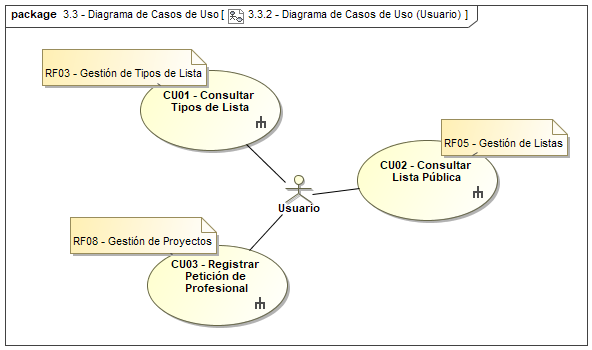
\includegraphics[width=150mm]{CasosDeUso_Usuario.png}
  \caption{Diagrama de Casos de uso (Usuario)}
  \label{fig:CasosDeUso_Usuario}
\end{figure}
\FloatBarrier
 \pagebreak

\addtocounter{tabla}{1}
El primer caso de uso (\textbf{\hyperref[tab:cuuConsultaTiposLst]{Tabla \arabic{tabla}}}) hace referencia al requisito funcional de \textbf{\hyperref[tab:rfGestTipoLst]{Gestión de Tipos de Lista (RF-3)}}, aunque solo a la parte de consultar su información. El usuario que la realiza no tiene que cumplir ninguna condición previa para ello.

\begin{table}[!htbp]
  \centering  \addtocounter{casouso}{1}
  \begin{tabular}{|l | p{100mm}|}
    \textbf{Caso de Uso}  & \textbf{Consultar Tipos de Lista} \\ \hline
    Resumen 		 & Un Usuario accede a la información de los tipos de lista para consultar su definición \\ \hline
    Actores  		 & Usuario \\ \hline
    Precondición  	 & No \\ \hline
    Postcondición  	 & Al Usuario se le han mostrado los tipos de lista y una descripción de cada uno de ellos \\ \hline
    Curso Normal   	 & \begin{enumerate}
	  \item El Usuario accede a TAP\textbackslash Tipos de Lista
	  \item El sistema muestra todas los tipos de lista y una descripción de cada una de ellas
    \end{enumerate}  \\ \hline
    Curso Alternativo  & No  \\ \hline
    Observaciones 	 & No es necesario iniciar sesión en el sistema para realizar esta acción  \\ \hline
  \end{tabular}
  \caption{Caso de Uso \arabic{casouso} - Consultar Tipos de Lista}
  \label{tab:cuuConsultaTiposLst}
\end{table}
\FloatBarrier

\addtocounter{tabla}{1}
Después tenemos una situación similar con la consulta de listas públicas (\textbf{\hyperref[tab:cuuConsultaLstPub]{Tabla \arabic{tabla}}}) de los requisitos de \textbf{\hyperref[tab:rfGestLst]{Gestión de Listas (RF-5)}}, pudiendo acceder solo a la consulta de listas públicas y la información que estas ofrecen de los colegiados. Para acceder a una de ellas será necesario que el interesado seleccione el tipo de lista y el territorio de la que desee consultar.

\begin{table}[!htbp]
  \centering  \addtocounter{casouso}{1}
  \begin{tabular}{|l | p{100mm}|}
    \textbf{Caso de Uso}  & \textbf{Consultar Lista Pública} \\ \hline
    Resumen 			 & Un Usuario accede a una lista pública de profesionales para contactar con un profesional colegiado concreto directamente \\ \hline
    Actores  		 & Usuario \\ \hline
    Precondición  	 & No \\ \hline
    Postcondición  	 & El sistema muestra los integrantes de la lista pública \\ \hline
    Curso Normal   	 & \begin{enumerate}
	  \item El Usuario accede a TAP\textbackslash Listas Públicas
	  \item El Usuario selecciona el tipo de lista y el territorio para las que busca solicitar la actuación
	  \item El sistema muestra un listado con la información de los profesionales inscritos en la lista pública para dicho tipo y territorio
    \end{enumerate}  \\ \hline
    Curso Alternativo  & No  \\ \hline
    Observaciones 	 & No es necesario iniciar sesión en el sistema para realizar esta acción  \\ \hline
  \end{tabular}
  \caption{Caso de Uso \arabic{casouso} - Consultar Lista Pública}
  \label{tab:cuuConsultaLstPub}
\end{table}
\FloatBarrier

\addtocounter{tabla}{1}
La función más compleja accesible por los Usuarios es la solicitud de un profesional para la realización de un servicio (\textbf{\hyperref[tab:cuuRegPeticProf]{Tabla \arabic{tabla}}}), relativo al requisito funcional \textbf{\hyperref[tab:rfGestProyectos]{Gestión de Proyectos (RF-8)}}. Para ello el Usuario debe introducir información suya de contacto y la descripción de lo que necesita. 

\begin{table}[!htbp]
  \centering  \addtocounter{casouso}{1}
  \begin{tabular}{|l | p{100mm}|}
    \textbf{Caso de Uso}  & \textbf{Registrar Petición de Profesional} \\ \hline
    Resumen 		 & Un Usuario solicita la actuación de un colegiado profesional y el sistema registra la petición \\ \hline
    Actores  		 & Usuario \\ \hline
    Precondición  	 & No \\ \hline
    Postcondición  	 & El sistema ha registrado la solicitud para la actuación de un profesional \\ \hline
    Curso Normal   	 & \begin{enumerate}
	  \item El Usuario accede a TAP\textbackslash Solicitud de Actuación
	  \item El Usuario introduce los datos de su solicitud
	  \item El sistema valida la información y registra la solicitud
	  \item El sistema confirma al usuario el procesamiento de su solicitud
    \end{enumerate}  \\ \hline
    Curso Alternativo  & \begin{enumerate}
	  \item El Usuario no rellena todos los campos obligatorios y el sistema le informa que debe completarlos
    \end{enumerate}  \\ \hline
    Observaciones 	 & No es necesario iniciar sesión en el sistema para realizar esta acción  \\ \hline
  \end{tabular}
  \caption{Caso de Uso \arabic{casouso} - Registrar Petición de Profesional}
  \label{tab:cuuRegPeticProf}
\end{table}
\FloatBarrier


\subsection{Perfil de Colegiado}

\addtocounter{figura}{1}
En este apartado se mostrarán los casos de uso de las funciones que pueden realizar los Colegiados (\textbf{\hyperref[fig:CasosDeUso_Colegiado]{Figura \arabic{figura}}}), que también serán accesibles para los Responsable.

\begin{figure}[!htbp]
  \centering
  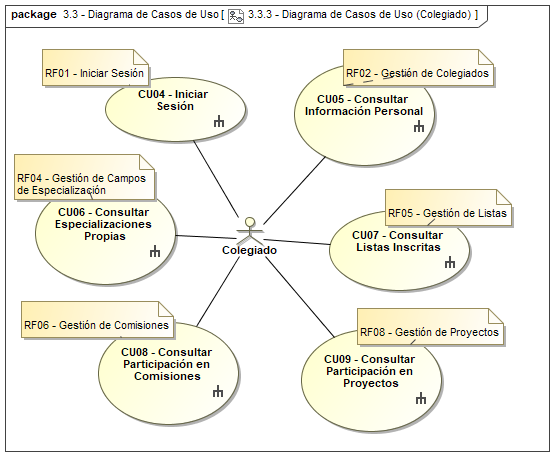
\includegraphics[width=150mm]{CasosDeUso_Colegiado.png}
  \caption{Diagrama de Casos de uso (Colegiado)}
  \label{fig:CasosDeUso_Colegiado}
\end{figure}
\FloatBarrier

\addtocounter{tabla}{1}
Para comenzar tenemos la función de iniciar sesión en el sistema (\textbf{\hyperref[tab:cucIniSes]{Tabla \arabic{tabla}}}), relacionada con el requisito funcional \textbf{\hyperref[tab:rfIniSes]{Iniciar Sesión (RF-1)}}. Para ello el colegiado tiene que introducir su número de colegiado y su contraseña.

\begin{table}[!htbp]
  \centering  \addtocounter{casouso}{1}
  \begin{tabular}{|l | p{100mm}|}
    \textbf{Caso de Uso}  & \textbf{Iniciar Sesión} \\ \hline
    Resumen 		 & Un Colegiado se identifica en el sistema con su número de colegiado y contraseña \\ \hline
    Actores  		 & Colegiado \\ \hline
    Precondición  	 & Estar desconectado, pero registrado en el sistema \\ \hline
    Postcondición  	 & El Colegiado ha iniciado sesión, y por tanto, ha sido identificado en el sistema \\ \hline
    Curso Normal   	 & \begin{enumerate}
	  \item El Colegiado accede a la Iniciar Sesión
	  \item El Colegiado introduce su número de colegiado y su contraseña
	  \item El sistema valida los datos introducidos
	  \item El sistema carga la entrada principal
    \end{enumerate}  \\ \hline
    Curso Alternativo  & \begin{enumerate}
	  \item La contraseña introducida no coincide con la del sistema
    \end{enumerate}  \\ \hline
    Observaciones 	 & Cuando los datos introducidos no son correctos, el sistema no especifica si el fallo radica en que el número de colegiado no está registrado o porque la contraseña es incorrecta  \\ \hline
  \end{tabular}
  \caption{Caso de Uso \arabic{casouso} - Iniciar Sesión}
  \label{tab:cucIniSes}
\end{table}
\FloatBarrier

\addtocounter{tabla}{1}
Los Colegiados, una vez identificados, podrán acceder a toda su información personal almacenada en el sistema (\textbf{\hyperref[tab:cucConsultaInfoPersonal]{Tabla \arabic{tabla}}}), cumpliendo con la consulta de Colegiados del requisito \textbf{\hyperref[tab:rfGestColeg]{Gestión de Colegiados (RF-2)}}, aunque no tendrán permiso para modificarla. Para la consulta deben acceder a su perfil de usuario.

\begin{table}[!htbp]
  \centering  \addtocounter{casouso}{1}
  \begin{tabular}{|l | p{100mm}|}
    \textbf{Caso de Uso}  & \textbf{Consultar Información Personal} \\ \hline
    Resumen 		 & Un Colegiado accede su perfil para consultar su información personal \\ \hline
    Actores  		 & Colegiado \\ \hline
    Precondición  	 & Haber iniciado sesión \\ \hline
    Postcondición  	 & El sistema muestra al Colegiado su información personal almacenada \\ \hline
    Curso Normal   	 & \begin{enumerate}
	  \item El Colegiado accede a Mi Perfil
	  \item El sistema muestra la información personal del Colegiado
    \end{enumerate}  \\ \hline
    Curso Alternativo  & No  \\ \hline
    Observaciones 	 & El colegiado tiene acceso a la consulta de sus datos, pero no a su modificación \\ \hline
  \end{tabular}
  \caption{Caso de Uso \arabic{casouso} - Consultar Información Personal}
  \label{tab:cucConsultaInfoPersonal}
\end{table}
\FloatBarrier

\addtocounter{tabla}{1}
Además tendrán la posibilidad de consultar las especializaciones que tiene confirmadas en su perfil (\textbf{\hyperref[tab:cucConsultaEspec]{Tabla \arabic{tabla}}}), relativa al requisito \textbf{\hyperref[tab:rfGestEspec]{Gestión de Campos de Especialización (RF-4)}}.

\begin{table}[!htbp]
  \centering  \addtocounter{casouso}{1}
  \begin{tabular}{|l | p{100mm}|}
    \textbf{Caso de Uso}  & \textbf{Consultar Especializaciones Propias} \\ \hline
    Resumen 		 & Un Colegiado accede a su perfil para consultar las especializaciones sobre las que tiene conocimientos \\ \hline
    Actores  		 & Colegiado \\ \hline
    Precondición  	 & Haber iniciado sesión \\ \hline
    Postcondición  	 & El sistema ha mostrado al Colegiado sus especializaciones \\ \hline
    Curso Normal   	 & \begin{enumerate}
	  \item El Colegiado accede a Colegiados\textbackslash Mis especializaciones
	  \item El sistema muestra sus especializaciones al colegiado
    \end{enumerate}  \\ \hline
    Curso Alternativo  & No \\ \hline
    Observaciones 	 & El colegiado solo puede consultar las especializaciones que le han sido asignadas \\ \hline
  \end{tabular}
  \caption{Caso de Uso \arabic{casouso} - Consultar Especializaciones Propias}
  \label{tab:cucConsultaEspec}
\end{table}
\FloatBarrier

\addtocounter{tabla}{1}
Relacionado con el requisito \textbf{\hyperref[tab:rfGestLst]{Gestión de Listas (RF-5)}}, los colegiados pueden consultar las listas en las que están inscritos y el número de colegiados que le preceden en turno en cada lista (\textbf{\hyperref[tab:cucConsultaLista]{Tabla \arabic{tabla}}}).

\begin{table}[!htbp]
  \centering  \addtocounter{casouso}{1}
  \begin{tabular}{|l | p{100mm}|}
    \textbf{Caso de Uso}  & \textbf{Consultar Listas Inscritas} \\ \hline
    Resumen 		 & Un Colegiado consulta el conjunto de listas en las que participa \\ \hline
    Actores  		 & Colegiado \\ \hline
    Precondición  	 & Haber iniciado sesión \\ \hline
    Postcondición  	 & El sistema muestra el conjunto de listas de profesionales y revisores en las que está inscrito el colegiado \\ \hline
    Curso Normal   	 & \begin{enumerate}
	  \item El Colegiado accede a Colegiados\textbackslash Mis listas
	  \item El sistema muestra las listas en las que participa el colegiado
    \end{enumerate}  \\ \hline
    Curso Alternativo  & No  \\ \hline
    Observaciones 	 & El colegiado solo puede consultar las lista en las que está inscrito \\ \hline
  \end{tabular}
  \caption{Caso de Uso \arabic{casouso} - Consultar Listas Inscritas}
  \label{tab:cucConsultaLista}
\end{table}
\FloatBarrier

\addtocounter{tabla}{1}
Después para los Colegiado tenemos la consulta de las comisiones en las que participa (\textbf{\hyperref[tab:cucConsultaComision]{Tabla \arabic{tabla}}}), relacionado con el requisito \textbf{\hyperref[tab:rfGestComTAP]{Gestión de Comisiones de TAP (RF-6)}}.

\begin{table}[!htbp]
  \centering  \addtocounter{casouso}{1}
  \begin{tabular}{|l | p{100mm}|}
    \textbf{Caso de Uso}  & \textbf{Consultar Participación en Comisiones} \\ \hline
    Resumen 		 & Un Colegiado consulta el conjunto de comisiones de TAP en las que está incluido \\ \hline
    Actores  		 & Colegiado \\ \hline
    Precondición  	 & Haber iniciado sesión \\ \hline
    Postcondición  	 & El sistema muestra el conjunto de las comisiones en las que participa \\ \hline
    Curso Normal   	 & \begin{enumerate}
	  \item El Colegiado accede a Colegiados\textbackslash Mis comisiones
	  \item El sistema muestra las comisiones de TAP en las que está incluido
    \end{enumerate}  \\ \hline
    Curso Alternativo  & No  \\ \hline
    Observaciones 	 & El colegiado solo puede consultar las comisiones en las que participa \\ \hline
  \end{tabular}
  \caption{Caso de Uso \arabic{casouso} - Consultar Participación en Comisiones}
  \label{tab:cucConsultaComision}
\end{table}
\FloatBarrier


\addtocounter{tabla}{1}
Como último caso de uso para los Colegiado tenemos la consulta de los proyectos que tiene asignados, ya sea como encargado, revisor o tutelador (\textbf{\hyperref[tab:cucConsultaProyectos]{Tabla \arabic{tabla}}}), relacionado con el requisito \textbf{\hyperref[tab:rfGestProyectos]{Gestión de Proyectos (RF-8)}}.

\begin{table}[!htbp]
  \centering  \addtocounter{casouso}{1}
  \begin{tabular}{|l | p{100mm}|}
    \textbf{Caso de Uso}  & \textbf{Consultar Participación en Proyectos} \\ \hline
    Resumen 		 & Un Colegiado consulta los proyectos que le han sido asignados \\ \hline
    Actores  		 & Colegiado \\ \hline
    Precondición  	 & Haber iniciado sesión \\ \hline
    Postcondición  	 & El sistema muestra el conjunto de proyectos que tiene asignados \\ \hline
    Curso Normal   	 & \begin{enumerate}
	  \item El Colegiado accede a Colegiados\textbackslash Mis proyectos
	  \item El sistema muestra los proyectos que tiene asignados
    \end{enumerate}  \\ \hline
    Curso Alternativo  & No  \\ \hline
    Observaciones 	 & El colegiado solo puede consultar los proyectos que le han sido asignados \\ \hline
  \end{tabular}
  \caption{Caso de Uso \arabic{casouso} - Consultar Participación en Proyectos}
  \label{tab:cucConsultaProyectos}
\end{table}
\FloatBarrier


\subsection{Perfil de Responsable}

\addtocounter{figura}{1}
En este apartado se definirán los casos de uso que solo podrán realizar los usuarios con perfil de Responsable, mostrados en la \textbf{\hyperref[fig:CasosDeUso_Responsable]{Figura \arabic{figura}}}.

\begin{figure}[!htbp]
  \centering
  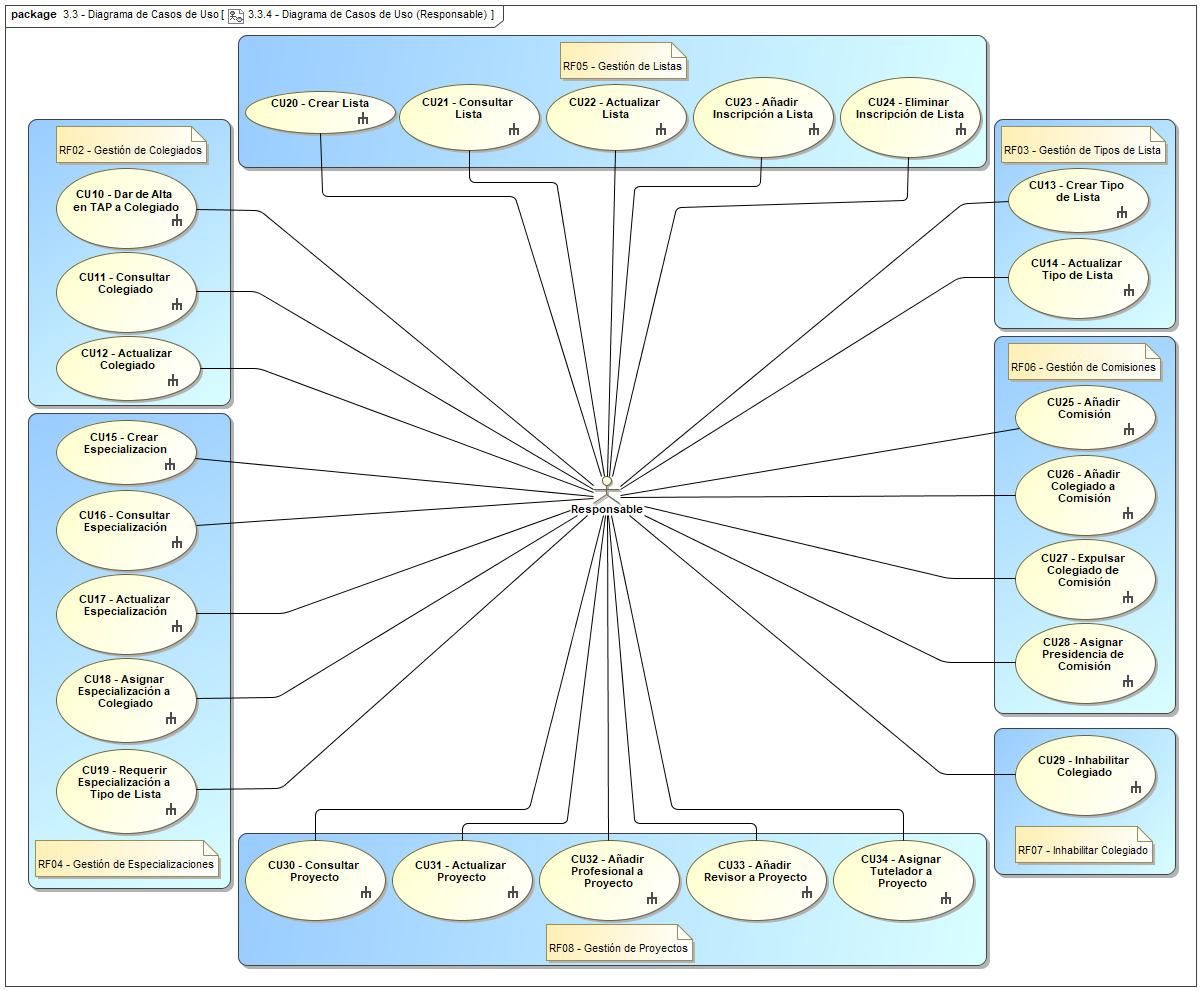
\includegraphics[width=150mm]{CasosDeUso_Responsable.png}
  \caption{Diagrama de Casos de uso (Responsable)}
  \label{fig:CasosDeUso_Responsable}
\end{figure}
\FloatBarrier


Los primeros son relativos al requisito funcional de \textbf{\hyperref[tab:rfGestColeg]{Gestión de Colegiados (RF-2)}}. Este incluye los casos de uso de:
\begin{itemize}
	\item \addtocounter{tabla}{1} Dar de alta un colegiado en el TAP (\textbf{\hyperref[tab:curColegAlta]{Tabla \arabic{tabla}}}).
		\begin{table}[!htbp]
		  \centering  \addtocounter{casouso}{1}
		  \begin{tabular}{|l | p{100mm}|}
		    \textbf{Caso de Uso}  & \textbf{Dar Alta en TAP a Colegiado} \\ \hline
		    Resumen 		 & Un Responsable introduce un colegiado en el sistema de TAP para que tenga acceso identificado \\ \hline
		    Actores  		 & Responsable \\ \hline
		    Precondición  	 & El colegiado no debe existir en el sistema  \\ \hline
		    Postcondición  	 & El colegiado ha sido registrado en el sistema de TAP \\ \hline
		    Curso Normal   	 & \begin{enumerate}
			  \item El Responsable accede a Administración\textbackslash Colegiados
			  \item El sistema muestra el listado de colegiados
			  \item El Responsable selecciona "Añadir Colegiado"
			  \item El Responsable introduce los datos del colegiado
			  \item El Responsable guarda los datos
			  \item El sistema valida la información y da de alta al colegiado
			  \item El sistema envía un correo electrónico al usuario con los datos de acceso a la plataforma
		    \end{enumerate}  \\ \hline
		    Curso Alternativo  & \begin{enumerate}
			  \item El sistema informa al Responsable el Colegiado ya existe
		    \end{enumerate}  \\ \hline
		    Observaciones 	 & En cualquier momento el Responsable puede abortar el proceso  \\ \hline
		  \end{tabular}
		  \caption{Caso de Uso \arabic{casouso} - Dar Alta en TAP a Colegiado}
		  \label{tab:curColegAlta}
		\end{table}
		\FloatBarrier
	
	\item \addtocounter{tabla}{1} Consultar los colegiados ya existentes (\textbf{\hyperref[tab:curConsultaInfoColeg]{Tabla \arabic{tabla}}}). A diferencia de la consulta de colegiados que pueden realizar los Colegiados, en este caso los Responsables tienen acceso a la información de todos los colegiados del sistema.
		\begin{table}[!htbp]
		  \centering  \addtocounter{casouso}{1}
		  \begin{tabular}{|l | p{100mm}|}
		    \textbf{Caso de Uso}  & \textbf{Consultar Información de Colegiado} \\ \hline
		    Resumen 		 & Un Responsable accede al perfil de un Colegiado para consultar su información \\ \hline
		    Actores  		 & Responsable \\ \hline
		    Precondición  	 & El Colegiado a consultar ya debe existir en el sistema \\ \hline
		    Postcondición  	 & El sistema muestra al Responsable la información del Colegiado \\ \hline
		    Curso Normal   	 & \begin{enumerate}
			  \item El Responsable accede a Administración\textbackslash Colegiados
			  \item El sistema muestra la lista de Colegiados
			  \item El Responsable busca al Colegiado en el sistema
			  \item El Responsable selecciona consultar el Colegiado
			  \item El sistema muestra la información del Colegiado
		    \end{enumerate}  \\ \hline
		    Curso Alternativo  & No  \\ \hline
		    Observaciones 	 & No \\ \hline
		  \end{tabular}
		  \caption{Caso de Uso \arabic{casouso} - Consultar Información de Colegiado}
		  \label{tab:curConsultaInfoColeg}
		\end{table}
		\FloatBarrier \pagebreak

	\item \addtocounter{tabla}{1} Modificar los colegiados ya creados en el sistema (\textbf{\hyperref[tab:curActualizarColeg]{Tabla \arabic{tabla}}}).
		\begin{table}[!htbp]
		  \centering \addtocounter{casouso}{1}
		  \begin{tabular}{|l | p{100mm}|}
		    \textbf{Caso de Uso}  & \textbf{Actualizar Información de un Colegiado} \\ \hline
		    Resumen 		 & Un Colegiado ya registrado precisa de modificar alguna información asociada a él \\ \hline
		    Actores  		 & Responsable \\ \hline
		    Precondición  	 & El Colegiado ya debe estar registrado en el sistema  \\ \hline
		    Postcondición  	 & La información del Colegiado se ha actualizado \\ \hline
		    Curso Normal   	 & \begin{enumerate}
			  \item El Responsable accede a Administración\textbackslash Colegiados
			  \item El sistema muestra al Responsable la lista de colegiados
			  \item El Responsable busca al Colegiado en el sistema
			  \item El Responsable selecciona actualizar el Colegiado
			  \item El sistema muestra la información del Colegiado
			  \item El Responsable introduce los datos nuevos
			  \item El sistema valida la información
			  \item El sistema modifica la información del Colegiado
		    \end{enumerate}  \\ \hline
		    Curso Alternativo  & \begin{enumerate}
			  \item El Usuario no rellena todos los campos obligatorios y el sistema le informa que debe completarlos
		    \end{enumerate}  \\ \hline
		    Observaciones 	 & El número de colegiado no permitirá su modificación  \\ \hline
		  \end{tabular}
		  \caption{Caso de Uso \arabic{casouso} - Actualizar Información de un Colegiado}
		  \label{tab:curActualizarColeg}
		\end{table}
		\FloatBarrier
\end{itemize}

Relativos al requisito de \textbf{\hyperref[tab:rfGestTipoLst]{Gestión de Tipos de Lista (RF-3)}} se definen los casos de uso para su creación y actualización:
\begin{itemize}
	\item \addtocounter{tabla}{1} Creación de un nuevo tipo de lista (\textbf{\hyperref[tab:curCrearTipoLst]{Tabla \arabic{tabla}}}). Es necesario que no exista antes una con el mismo nombre.
		\begin{table}[!htbp]
		  \centering  \addtocounter{casouso}{1}
		  \begin{tabular}{|l | p{100mm}|}
		    \textbf{Caso de Uso}  & \textbf{Crear Nuevo Tipo de Lista} \\ \hline
		    Resumen 		 & Se debe crear un nuevo tipo de lista \\ \hline
		    Actores  		 & Responsable \\ \hline
		    Precondición  	 & El tipo de lista nuevo no existe en el sistema  \\ \hline
		    Postcondición  	 & El sistema ha creado el nuevo tipo de lista \\ \hline
		    Curso Normal   	 & \begin{enumerate}
			  \item El Responsable accede a Administración\textbackslash Tipos de Lista
			  \item El sistema muestra los tipos de lista.
			  \item El Responsable selecciona "Añadir"
			  \item El Responsable introduce los datos del nuevo tipo
			  \item El Responsable guarda los datos
			  \item El sistema valida la información
			  \item El sistema crea el nuevo tipo
		    \end{enumerate}  \\ \hline
		    Curso Alternativo  & \begin{enumerate}
			  \item El sistema informa al Responsable que ya existe un tipo de lista con ese nombre
		    \end{enumerate}  \\ \hline
		    Observaciones 	 & En cualquier momento el Responsable puede abortar el proceso  \\ \hline
		  \end{tabular}
		  \caption{Caso de Uso \arabic{casouso} - Crear Nuevo Tipo de Lista}
		  \label{tab:curCrearTipoLst}
		\end{table}
		\FloatBarrier
	
	\item \addtocounter{tabla}{1} Actualizar tipo de lista ya creado (\textbf{\hyperref[tab:curActualizarTipoLst]{Tabla \arabic{tabla}}}).
		\begin{table}[!htbp]
		  \centering  \addtocounter{casouso}{1}
		  \begin{tabular}{|l | p{100mm}|}
		    \textbf{Caso de Uso}  & \textbf{Actualizar Tipo de Lista} \\ \hline
		    Resumen 		 & Un tipo de lista ya registrado precisa de modificar su información \\ \hline
		    Actores  		 & Responsable \\ \hline
		    Precondición  	 & El tipo de lista ya debe estar creado en el sistema  \\ \hline
		    Postcondición  	 & La información del tipo de lista ha sido modificada \\ \hline
		    Curso Normal   	 & \begin{enumerate}
			  \item El Responsable accede a Administración\textbackslash Tipo de Lista
			  \item El Responsable busca el tipo de lista en el sistema
			  \item El Responsable selecciona "Modificar" un tipo de lista
			  \item El sistema muestra la información del tipo de lista
			  \item El Responsable introduce los datos nuevos del tipo de lista
			  \item El sistema valida la información y lo da por actualizado
		    \end{enumerate}  \\ \hline
		    Curso Alternativo  & \begin{enumerate}
			  \item El sistema informa al Responsable que el campo "nombre" no puede estar vacío si quiere continuar la modificación
		    \end{enumerate}  \\ \hline
		    Observaciones 	 & No  \\ \hline
		  \end{tabular}
		  \caption{Caso de Uso \arabic{casouso} - Actualizar Tipo de Lista}
		  \label{tab:curActualizarTipoLst}
		\end{table}
		\FloatBarrier
\end{itemize}


En cuanto al requisito de \textbf{\hyperref[tab:rfGestEspec]{Gestión de Campos de Especialización (RF-4)}} se definen cinco nuevos casos de uso:
\begin{itemize}
	\item \addtocounter{tabla}{1} Creación de nueva especialización (\textbf{\hyperref[tab:curCrearEspec]{Tabla \arabic{tabla}}}). Es necesario que no exista antes una con el mismo nombre.
		\begin{table}[!htbp]
		  \centering  \addtocounter{casouso}{1}
		  \begin{tabular}{|l | p{100mm}|}
		    \textbf{Caso de Uso}  & \textbf{Crear una Nueva Especialización} \\ \hline
		    Resumen 		 & Se debe crear una nueva especialización \\ \hline
		    Actores  		 & Responsable \\ \hline
		    Precondición  	 & La especialización no existe en el sistema  \\ \hline
		    Postcondición  	 & El sistema ha creado la nueva especialización \\ \hline
		    Curso Normal   	 & \begin{enumerate}
			  \item El Responsable accede a Administración\textbackslash Especializaciones
			  \item El sistema muestra las especializaciones ya existentes
			  \item El Responsable selecciona "Añadir"
			  \item El Responsable introduce los datos de la nueva especialización
			  \item El Responsable guarda los datos
			  \item El sistema valida la información
			  \item El sistema crea la nueva especialización
		    \end{enumerate}  \\ \hline
		    Curso Alternativo  & \begin{enumerate}
			  \item El Usuario no rellena todos los campos obligatorios y el sistema le informa que debe completarlos
		    \end{enumerate}  \\ \hline
		    Observaciones 	 & En cualquier momento el Responsable puede abortar la creación de la nueva especialización  \\ 		\hline
		  \end{tabular}
		  \caption{Caso de Uso \arabic{casouso} - Crear una Nueva Especialización }
		  \label{tab:curCrearEspec}
		\end{table}
		\FloatBarrier
	
	\item \addtocounter{tabla}{1} Consultar especializaciones (\textbf{\hyperref[tab:curConsultarEspec]{Tabla \arabic{tabla}}}).
		\begin{table}[!htbp]
		  \centering  \addtocounter{casouso}{1}
		  \begin{tabular}{|l | p{100mm}|}
		    \textbf{Caso de Uso}  & \textbf{Consultar una Especialización} \\ \hline
		    Resumen 		 & Un Responsable accede a la información de una especialización \\ \hline
		    Actores  		 & Responsable \\ \hline
		    Precondición  	 & La especialización ya debe estar creada en el sistema  \\ \hline
		    Postcondición  	 & El sistema ha mostrado la información de la especialización al Responsable \\ \hline
		    Curso Normal   	 & \begin{enumerate}
			  \item El Responsable accede a Administración\textbackslash Especializaciones
			  \item El Responsable busca la especialización en el sistema
			  \item El Responsable selecciona "Consultar"
			  \item El sistema muestra la información de la especialización
		    \end{enumerate}  \\ \hline
		    Curso Alternativo  & No  \\ \hline
		    Observaciones 	 & No  \\ \hline
		  \end{tabular}
		  \caption{Caso de Uso \arabic{casouso} - Consultar una Especialización}
		  \label{tab:curConsultarEspec}
		\end{table}
		\FloatBarrier
	
	\item \addtocounter{tabla}{1} Actualizar especialización ya creada (\textbf{\hyperref[tab:curActualizarEspec]{Tabla \arabic{tabla}}}).
		\begin{table}[!htbp]
		  \centering  \addtocounter{casouso}{1}
		  \begin{tabular}{|l | p{100mm}|}
		    \textbf{Caso de Uso}  & \textbf{Actualizar Información de una Especialización} \\ \hline
		    Resumen 		 & Una especialización ya registrada precisa de modificar alguna información asociada a ella \\ \hline
		    Actores  		 & Responsable \\ \hline
		    Precondición  	 & La especialización ya debe estar creada en el sistema  \\ \hline
		    Postcondición  	 & La información de la especialización ha sido modificada \\ \hline
		    Curso Normal   	 & \begin{enumerate}
			  \item El Responsable accede a Administración\textbackslash Especializaciones
			  \item El Responsable busca la especialización en el sistema
			  \item El Responsable selecciona "Modificar"
			  \item El sistema muestra la información de la especialización
			  \item El Responsable introduce los datos nuevos de la especialización
			  \item El sistema valida la información y la da por actualizada
		    \end{enumerate}  \\ \hline
		    Curso Alternativo  & \begin{enumerate}
			  \item El sistema informa al Responsable que el campo "nombre" no puede estar vacío si quiere continuar la actualización de la especialización
		    \end{enumerate}  \\ \hline
		    Observaciones 	 & No  \\ \hline
		  \end{tabular}
		  \caption{Caso de Uso \arabic{casouso} - Actualizar Información de una Especialización}
		  \label{tab:curActualizarEspec}
		\end{table}
		\FloatBarrier
		
	\item \addtocounter{tabla}{1} Asignar especialización a colegiado (\textbf{\hyperref[tab:curAsignarEspecColeg]{Tabla \arabic{tabla}}}). Esto servirá para registrar los conocimientos que poseen los colegiados una vez los acrediten.
		\begin{table}[!htbp]
		  \centering  \addtocounter{casouso}{1}
		  \begin{tabular}{|l | p{100mm}|}
		    \textbf{Caso de Uso}  & \textbf{Asignar Especialización a Colegiado} \\ \hline
		    Resumen 		 & Un Responsable asigna una especialización a un colegiado \\ \hline
		    Actores  		 & Responsable \\ \hline
		    Precondición  	 & La especialización y el colegiado deben existir en el sistema y no estar ya asignada  \\ \hline
		    Postcondición  	 & Se ha registrado los conocimientos del colegiado en la especialización \\ \hline
		    Curso Normal   	 & \begin{enumerate}
			  \item El Responsable accede a Administración\textbackslash Colegiados
			  \item El Responsable busca el colegiado en el sistema
			  \item El Responsable selecciona "Modificar"
			  \item El sistema muestra la información del usuario
			  \item El Responsable selecciona "Añadir Especialización"
			  \item El sistema muestra las distintas especializaciones
			  \item El Responsable selecciona la especialización a añadir
			  \item El sistema confirma la asignación
		    \end{enumerate}  \\ \hline
		    Curso Alternativo  & No  \\ \hline
		    Observaciones 	 & No se puede repetir una asignación en el mismo colegiado  \\ \hline
		  \end{tabular}
		  \caption{Caso de Uso \arabic{casouso} - Asignar Especialización a Colegiado}
		  \label{tab:curAsignarEspecColeg}
		\end{table}
		\FloatBarrier
		
	\item \addtocounter{tabla}{1} Requerir especialización a tipo de lista (\textbf{\hyperref[tab:curRequerirEspecTipoLst]{Tabla \arabic{tabla}}}). De esta forma se establecen los conocimientos necesarios para pertenecer a las listas de ese tipo.
		\begin{table}[!htbp]
		  \centering  \addtocounter{casouso}{1}
		  \begin{tabular}{|l | p{100mm}|}
		    \textbf{Caso de Uso}  & \textbf{Requerir Especialización a Tipo de Lista} \\ \hline
		    Resumen 		 & Un Responsable establece una especialización como requisito de un tipo de lista \\ \hline
		    Actores  		 & Responsable \\ \hline
		    Precondición  	 & La especialización no es requisito del tipo de lista  \\ \hline
		    Postcondición  	 & Se ha establecido la especialización como requisito para pertenecer a las listas ese tipo \\ \hline
		    Curso Normal   	 & \begin{enumerate}
			  \item El Responsable accede a Administración\textbackslash Tipos de Lista
			  \item El sistema muestra los tipos de lista
			  \item El Responsable selecciona "Modificar"
			  \item El sistema muestra la información de dicho tipo
			  \item El Responsable selecciona "Añadir especialización"
			  \item El sistema muestra las distintas especializaciones
			  \item El Responsable selecciona la especialización a requerir
			  \item El sistema confirma la asignación del requisito
		    \end{enumerate}  \\ \hline
		    Curso Alternativo  & No  \\ \hline
		    Observaciones 	 & No se puede requerir a un tipo de lista la misma especialización más de una vez  \\ \hline
		  \end{tabular}
		  \caption{Caso de Uso \arabic{casouso} - Requerir Especialización a Tipo de Lista}
		  \label{tab:curRequerirEspecTipoLst}
		\end{table}
		\FloatBarrier
\end{itemize}

Del requisito \textbf{\hyperref[tab:rfGestLst]{Gestión de Listas (RF-5)}} aparecen cinco nuevos casos de uso:
\begin{itemize}
	\item \addtocounter{tabla}{1} Crear una lista (\textbf{\hyperref[tab:curCrearLista]{Tabla \arabic{tabla}}}).
		\begin{table}[!htbp]
		  \centering  \addtocounter{casouso}{1}
		  \begin{tabular}{|l | p{100mm}|}
		    \textbf{Caso de Uso}  & \textbf{Crear Lista} \\ \hline
		    Resumen 		 & Un Responsable añade una nueva lista al sistema. Puede ser de profesionales o de revisores \\ \hline
		    Actores  		 & Responsable \\ \hline
		    Precondición  	 & No debe existir ninguna lista que coincida en tipo, pública/privada y territorio con la nueva  \\ \hline
		    Postcondición  	 & La lista ha sido creada \\ \hline
		    Curso Normal   	 & \begin{enumerate}
			  \item El Responsable accede a Administración\textbackslash Listas
			  \item El sistema muestra el conjunto de listas existentes
			  \item El Responsable selecciona "Añadir"
			  \item El Responsable introduce los datos de la lista
			  \item El Responsable guarda los datos
			  \item El sistema valida la información y crea la lista
		    \end{enumerate}  \\ \hline
		    Curso Alternativo  & \begin{enumerate}
			  \item El sistema informa al Responsable que ya existe una lista con esas características
		    \end{enumerate}  \\ \hline
		    Observaciones 	 & En cualquier momento el Responsable puede abortar el proceso  \\ \hline
		  \end{tabular}
		  \caption{Caso de Uso \arabic{casouso} - Crear Lista}
		  \label{tab:curCrearLista}
		\end{table}
		\FloatBarrier
	
	\item \addtocounter{tabla}{1} Consultar las listas ya existentes (\textbf{\hyperref[tab:curConsultarLista]{Tabla \arabic{tabla}}}). A diferencia de la consulta de listas públicas a la que tienen acceso los Usuario, en este caso los Responsables tienen acceso a la información de todas las lista del sistema, sean públicas o privadas y de profesionales o de revisores.
		\begin{table}[!htbp]
		  \centering  \addtocounter{casouso}{1}
		  \begin{tabular}{|l | p{100mm}|}
		    \textbf{Caso de Uso}  & \textbf{Consultar Lista} \\ \hline
		    Resumen 		 & Un Responsable accede a la información de una de las listas \\ \hline
		    Actores  		 & Responsable \\ \hline
		    Precondición  	 & Haber iniciado sesión con perfil de Responsable \\ \hline
		    Postcondición  	 & El sistema muestra al Responsable la información de la lista \\ \hline
		    Curso Normal   	 & \begin{enumerate}
			  \item El Responsable accede a Administración\textbackslash Listas
			  \item El sistema muestra el conjunto de listas existentes
			  \item El Responsable busca la lista
			  \item El Responsable selecciona "Consultar"
			  \item El sistema muestra la información de la lista
		    \end{enumerate}  \\ \hline
		    Curso Alternativo  & No  \\ \hline
		    Observaciones 	 & No \\ \hline
		  \end{tabular}
		  \caption{Caso de Uso \arabic{casouso} - Consultar Lista}
		  \label{tab:curConsultarLista}
		\end{table}
		\FloatBarrier \pagebreak

	\item \addtocounter{tabla}{1} Modificar las listas ya creadas en el sistema (\textbf{\hyperref[tab:curActualizarLista]{Tabla \arabic{tabla}}}).
		\begin{table}[!htbp]
		  \centering \addtocounter{casouso}{1}
		  \begin{tabular}{|l | p{100mm}|}
		    \textbf{Caso de Uso}  & \textbf{Actualizar Información de una Lista} \\ \hline
		    Resumen 		 & Una lista ya creada precisa de modificar alguna información asociada a ella \\ \hline
		    Actores  		 & Responsable \\ \hline
		    Precondición  	 & La lista ya debe existir en el sistema  \\ \hline
		    Postcondición  	 & La información de la lista se ha actualizado \\ \hline
		    Curso Normal   	 & \begin{enumerate}
			  \item El Responsable accede a Administración\textbackslash Lista
			  \item El sistema muestra el conjunto de listas existentes
			  \item El Responsable busca la lista
			  \item El Responsable selecciona "Modificar"
			  \item El sistema muestra la información de la lista
			  \item El Responsable introduce los datos nuevos
			  \item El sistema valida la información
			  \item El sistema modifica la información de la lista
		    \end{enumerate}  \\ \hline
		    Curso Alternativo  & \begin{enumerate}
			  \item El sistema informa al Responsable que ya existe una lista con esas características
		    \end{enumerate}  \\ \hline
		    Observaciones 	 & El identificador de la lista no permitirá su modificación  \\ \hline
		  \end{tabular}
		  \caption{Caso de Uso \arabic{casouso} - Actualizar Información de una Lista}
		  \label{tab:curActualizarLista}
		\end{table}
		\FloatBarrier
		
	\item \addtocounter{tabla}{1} Añadir inscripciones de colegiados a las listas (\textbf{\hyperref[tab:curCrearInscrLst]{Tabla \arabic{tabla}}}). Los Responsables se basarán en los criterios del Reglamento de TAP\cite{reglamentotapcpiia} para ver si el Colegiado en cuestión cumple lo necesario para forma parte de la lista. Además, el colegiado deberá tener conocimientos en todas las especializaciones requeridas al tipo de lista seleccionada.
		\begin{table}[!htbp]
		  \centering  \addtocounter{casouso}{1}
		  \begin{tabular}{|l | p{100mm}|}
		    \textbf{Caso de Uso}  & \textbf{Añadir Inscripción a Lista} \\ \hline
		    Resumen 		 & El Responsable añade la inscripción de un colegiado a una lista \\ \hline
		    Actores  		 & Responsable \\ \hline
		    Precondición  	 & El Colegiado y la lista deben existir previamente y el Colegiado debe tener conocimiento en todas las especializaciones que requiere la lista  \\ \hline
		    Postcondición  	 & El sistema ha registrado la inscripción del Colegiado en la lista \\ \hline
		    Curso Normal   	 & \begin{enumerate}
			  \item El Responsable accede a Administración\textbackslash Colegiados
			  \item El sistema muestra la lista de colegiados
			  \item El Responsable busca el colegiado en el sistema
			  \item El Responsable selecciona "Modificar"
			  \item El sistema muestra la información del colegiado
			  \item El Responsable selecciona "Añadir Inscripción"
			  \item El sistema muestra las distintas listas
			  \item El Responsable selecciona una lista
			  \item El sistema registra la inscripción
		    \end{enumerate}  \\ \hline
		    Curso Alternativo  & \begin{enumerate}
			  \item El sistema informa que el colegiado no cuenta con conocimientos suficientes para participar en la lista
		    \end{enumerate}  \\ \hline
		    Observaciones 	 & Si no tiene asignado conocimientos en todas las especializaciones requeridas no se puede registrar la inscripción \\ \hline
		  \end{tabular}
		  \caption{Caso de Uso \arabic{casouso} - Añadir Inscripción a Lista}
		  \label{tab:curCrearInscrLst}
		\end{table}
		\FloatBarrier
		
		\item \addtocounter{tabla}{1} Eliminar inscripción en lista de un colegiado (\textbf{\hyperref[tab:curEliminarInscrLst]{Tabla \arabic{tabla}}}). Esto ocurrirá cuando los colegiados soliciten su baja de alguna de las listas en las que estén inscritos, ya que la pertenencia a las listas es totalmente voluntaria.
		\begin{table}[!htbp]
		  \centering  \addtocounter{casouso}{1}
		  \begin{tabular}{|l | p{100mm}|}
		    \textbf{Caso de Uso}  & \textbf{Eliminar Inscripción en Lista} \\ \hline
		    Resumen 		 & El Responsable borra la inscripción de un colegiado en una lista \\ \hline
		    Actores  		 & Responsable \\ \hline
		    Precondición  	 & El Colegiado debe estar inscrito en la lista  \\ \hline
		    Postcondición  	 & El sistema ha registrado la inscripción del Colegiado en la lista \\ \hline
		    Curso Normal   	 & \begin{enumerate}
			  \item El Responsable accede a Administración\textbackslash Colegiados
			  \item El sistema muestra la lista de colegiados
			  \item El Responsable busca el colegiado en el sistema
			  \item El Responsable selecciona "Modificar"
			  \item El sistema muestra la información del colegiado
			  \item El Responsable busca la lista de la que quiere expulsarlo
			  \item El Responsable selecciona "Expulsar"
			  \item El sistema borra la inscripción
		    \end{enumerate}  \\ \hline
		    Curso Alternativo  & No  \\ \hline
		    Observaciones 	 & No \\ \hline
		  \end{tabular}
		  \caption{Caso de Uso \arabic{casouso} - Eliminar Inscripción en Lista}
		  \label{tab:curEliminarInscrLst}
		\end{table}
		\FloatBarrier
\end{itemize}

Relacionados con el requisito funcional de \textbf{\hyperref[tab:rfGestComTAP]{Gestión de Comisiones de TAP (RF-6)}} existen cuatro casos de uso para el perfil de Responsable:
\begin{itemize}
	\item \addtocounter{tabla}{1} Añadir una comisión (\textbf{\hyperref[tab:curCrearComision]{Tabla \arabic{tabla}}}).
		\begin{table}[!htbp]
		  \centering  \addtocounter{casouso}{1}
		  \begin{tabular}{|l | p{100mm}|}
		    \textbf{Caso de Uso}  & \textbf{Añadir Comisión} \\ \hline
		    Resumen 		 & Un Responsable añade una nueva comisión al sistema \\ \hline
		    Actores  		 & Responsable \\ \hline
		    Precondición  	 & No \\ \hline
		    Postcondición  	 & La comisión ha sido creada \\ \hline
		    Curso Normal   	 & \begin{enumerate}
			  \item El Responsable accede a Administración\textbackslash Comisiones
			  \item El sistema muestra el conjunto de comisiones existentes
			  \item El Responsable selecciona "Añadir"
			  \item El Responsable introduce los datos de la comisión
			  \item El Responsable guarda los datos
			  \item El sistema valida la información y añade la comisión
		    \end{enumerate}  \\ \hline
		    Curso Alternativo  & No  \\ \hline
		    Observaciones 	 & En cualquier momento el Responsable puede abortar el proceso  \\ \hline
		  \end{tabular}
		  \caption{Caso de Uso \arabic{casouso} - Añadir Comisión}
		  \label{tab:curCrearComision}
		\end{table}
		\FloatBarrier
		
	\item \addtocounter{tabla}{1} Añadir colegiados a una comisión de TAP (\textbf{\hyperref[tab:curIncluirColegComisionTAP]{Tabla \arabic{tabla}}}). De igual forma que en las inscripciones a listas, el Responsable deberá verificar que el colegiado en cuestión cumple con lo requerido en el Reglamento de TAP\cite{reglamentotapcpiia} para formar parte de la comisión.
		\begin{table}[!htbp]
		  \centering  \addtocounter{casouso}{1}
		  \begin{tabular}{|l | p{100mm}|}
		    \textbf{Caso de Uso}  & \textbf{Añadir Colegiado a la Comisión de TAP} \\ \hline
		    Resumen 		 & El Responsable añade un Colegiado a la comisión de TAP \\ \hline
		    Actores  		 & Responsable \\ \hline
		    Precondición  	 & El colegiado debe formar parte de una lista gestionada por la comisión  \\ \hline
		    Postcondición  	 & El sistema ha incluido al Colegiado en la comisión de TAP \\ \hline
		    Curso Normal   	 & \begin{enumerate}
			  \item El Responsable accede a Administración\textbackslash Colegiados
			  \item El sistema muestra la lista de colegiados
			  \item El Responsable busca el colegiado en el sistema
			  \item El Responsable selecciona "Modificar"
			  \item El sistema muestra la información del colegiado
			  \item El Responsable selecciona "Añadir a Comisión"
			  \item El sistema muestra las distintas comisiones
			  \item El Responsable selecciona una comisión
			  \item El sistema registra la inclusión
		    \end{enumerate}  \\ \hline
		    Curso Alternativo  & \begin{enumerate}
			  \item El Colegiado no forma parte de ninguna lista gestionada por dicha comisión y no se puede añadir
		    \end{enumerate}  \\ \hline
		    Observaciones 	 & No  \\ \hline
		  \end{tabular}
		  \caption{Caso de Uso \arabic{casouso} - Añadir Colegiado a la Comisión de TAP}
		  \label{tab:curIncluirColegComisionTAP}
		\end{table}
		\FloatBarrier \pagebreak

	\item \addtocounter{tabla}{1} Expulsar colegiados de una comisión de TAP (\textbf{\hyperref[tab:curExpulsarColegComisionTAP]{Tabla \arabic{tabla}}}). Como ocurría con las inscripciones en listas, la pertenencia a una comisión de TAP es voluntaria y el colegiado puede solicitar su salida de la misma en cualquier momento.
		\begin{table}[!htbp]
		  \centering  \addtocounter{casouso}{1}
		  \begin{tabular}{|l | p{100mm}|}
		    \textbf{Caso de Uso}  & \textbf{Expulsar Colegiado de la Comisión de TAP} \\ \hline
		    Resumen 		 & El Responsable expulsa a un Colegiado de una comisión de TAP \\ \hline
		    Actores  		 & Responsable \\ \hline
		    Precondición  	 & El Colegiado es miembro de la comisión  \\ \hline
		    Postcondición  	 & El Colegiado ya no forma parte de la comisión de TAP \\ \hline
		    Curso Normal   	 & \begin{enumerate}
		      \item El Responsable accede a Administración\textbackslash Colegiados
			  \item El sistema muestra la lista de colegiados
			  \item El Responsable busca el colegiado en el sistema
			  \item El Responsable selecciona "Modificar"
			  \item El sistema muestra la información del colegiado
			  \item El Responsable busca la comisión de la que quiere expulsarlo
			  \item El Responsable selecciona "Expulsar"
			  \item El sistema borra la inclusión en la lista
		    \end{enumerate}  \\ \hline
		    Curso Alternativo  & \begin{enumerate}
			  \item El Colegiado no forma parte de ninguna comisión
		    \end{enumerate}  \\ \hline
		    Observaciones 	 & No  \\ \hline
		  \end{tabular}
		  \caption{Caso de Uso \arabic{casouso} - Expulsar Colegiado de la Comisión de TAP}
		  \label{tab:curExpulsarColegComisionTAP}
		\end{table}
		\FloatBarrier \pagebreak

	\item \addtocounter{tabla}{1} Asignar la presidencia de una comisión de TAP a uno de sus miembros (\textbf{\hyperref[tab:curAsignarPresidenciaComisionTAP]{Tabla \arabic{tabla}}})
		\begin{table}[!htbp]
		  \centering \addtocounter{casouso}{1}
		  \begin{tabular}{|l | p{100mm}|}
		    \textbf{Caso de Uso}  & \textbf{Asignar Presidencia de Comisión de TAP} \\ \hline
		    Resumen 		 & El Responsable asigna a un miembro de la comisión el papel de presidente de la misma \\ \hline
		    Actores  		 & Responsable \\ \hline
		    Precondición  	 & El que será presidente debe pertenecer a la comisión \\ \hline
		    Postcondición  	 & El sistema intercambia la presidencia de la comisión del antiguo presidente al nuevo Colegiado seleccionado \\ \hline
		    Curso Normal   	 & \begin{enumerate}
			  \item El Responsable accede a Administración\textbackslash Comisiones
			  \item El sistema muestra la lista de comisiones de TAP
			  \item El Responsable busca la comisión
			  \item El Responsable selecciona "Modificar"
			  \item El sistema muestra la información de la comisión seleccionada
			  \item El Responsable establece un nuevo miembro como presidente de la comisión
			  \item El sistema valida y registra el cambio de presidencia
		    \end{enumerate}  \\ \hline
		    Curso Alternativo  & No  \\ \hline
		    Observaciones 	 & El Responsable tiene la opción de cancelar el cambio mientras no lo haya confirmado  \\ \hline
		  \end{tabular}
		  \caption{Caso de Uso \arabic{casouso} - Asignar Presidencia de Comisión de TAP}
		  \label{tab:curAsignarPresidenciaComisionTAP}
		\end{table}
		\FloatBarrier
\end{itemize}

\addtocounter{tabla}{1}
El caso de uso de inhabilitar colegiado (\textbf{\hyperref[tab:curInhabilitar]{Tabla \arabic{tabla}}}), correspondiente al requisito funcional \textbf{\hyperref[tab:rfInhabilitar]{Inhabilitar Colegiados (RF-7)}} se encarga de expulsar al colegiado de todas las listas y comisiones de las que forma parte.

\begin{table}[!htbp]
  \centering  \addtocounter{casouso}{1}
  \begin{tabular}{|l | p{100mm}|}
    \textbf{Caso de Uso}  & \textbf{Inhabilitar Colegiado} \\ \hline
    Resumen 		 & El Responsable registra la sanción de inhabilitación a un Colegiado \\ \hline
    Actores  		 & Responsable \\ \hline
    Precondición  	 & El Colegiado debe estar registrado en el sistema \\ \hline
    Postcondición  	 & El sistema ha registrado la sanción de inhabilitación y ha expulsado al Colegiado de todas las listas y comisiones en las que estuviese inscrito \\ \hline
    Curso Normal   	 & \begin{enumerate}
	  \item El Responsable accede a Administración\textbackslash Colegiados
	  \item El sistema muestra la lista de colegiados
	  \item El Responsable busca el colegiado en el sistema
	  \item El Responsable selecciona "Modificar"
	  \item El sistema muestra la información del colegiado
	  \item El Responsable establece una fecha al campo "Fin de Inhabilitación"
	  \item El Responsable selecciona "Actualizar"
	  \item El sistema expulsa al Colegiado de todas las listas y comisiones
	  \item El sistema confirma el cambio
    \end{enumerate}  \\ \hline
    Curso Alternativo  & No  \\ \hline
    Observaciones 	 & No \\ \hline
  \end{tabular}
  \caption{Caso de Uso \arabic{casouso} - Inhabilitar Colegiado}
  \label{tab:curInhabilitar}
\end{table}
\FloatBarrier

\addtocounter{tabla}{1}
Finalmente, y de acuerdo al requisito \textbf{\hyperref[tab:rfGestProyectos]{Gestión de Proyectos (RF-8)}}, encontramos los últimos cinco casos de uso:
\begin{itemize}
	\item \addtocounter{tabla}{1} Consultar los proyectos existentes (\textbf{\hyperref[tab:curConsultarProyectos]{Tabla \arabic{tabla}}}).
		\begin{table}[!htbp]
		  \centering  \addtocounter{casouso}{1}
		  \begin{tabular}{|l | p{100mm}|}
		    \textbf{Caso de Uso}  & \textbf{Consultar Proyecto} \\ \hline
		    Resumen 		 & Un Responsable accede a la información de un proyecto \\ \hline
		    Actores  		 & Responsable \\ \hline
		    Precondición  	 & El proyecto ya debe existir \\ \hline
		    Postcondición  	 & El sistema muestra al Responsable la información del proyecto \\ \hline
		    Curso Normal   	 & \begin{enumerate}
			  \item El Responsable accede a Administración\textbackslash Proyectos
			  \item El sistema muestra el conjunto de proyectos existentes
			  \item El Responsable busca el proyecto
			  \item El Responsable selecciona "Consultar"
			  \item El sistema muestra la información del proyecto
		    \end{enumerate}  \\ \hline
		    Curso Alternativo  & No  \\ \hline
		    Observaciones 	 & No  \\ \hline
		  \end{tabular}
		  \caption{Caso de Uso \arabic{casouso} - Consultar Proyectos}
		  \label{tab:curConsultarProyectos}
		\end{table}
		\FloatBarrier
		
	\item \addtocounter{tabla}{1} Actualizar estado de un proyecto (\textbf{\hyperref[tab:curActualizarProyecto]{Tabla \arabic{tabla}}}). Esto incluye la modificación del estado de la solicitud, del servicio o del visado.
		\begin{table}[!htbp]
		  \centering  \addtocounter{casouso}{1}
		  \begin{tabular}{|l | p{100mm}|}
		    \textbf{Caso de Uso}  & \textbf{Actualizar Estado del Proyecto} \\ \hline
		    Resumen 		 & El Responsable cambia el estado del proyecto \\ \hline
		    Actores  		 & Responsable \\ \hline
		    Precondición  	 & El proyecto ya debe existir  \\ \hline
		    Postcondición  	 & El estado del proyecto ha sido modificado \\ \hline
		    Curso Normal   	 & \begin{enumerate}
			  \item El Responsable accede a Administración\textbackslash Proyectos
			  \item El sistema muestra la lista de proyectos
			  \item El Responsable busca el proyecto
			  \item El Responsable selecciona "Modificar"
			  \item El sistema muestra la información del proyecto
			  \item El Responsable cambia alguno de los estados
			  \item El Responsable selecciona "Actualizar Proyecto"
			  \item El sistema modifica el estado
		    \end{enumerate}  \\ \hline
		    Curso Alternativo  & No  \\ \hline
		    Observaciones 	 & No  \\ \hline
		  \end{tabular}
		  \caption{Caso de Uso \arabic{casouso} - Actualizar Estado del Proyecto}
		  \label{tab:curActualizarProyecto}
		\end{table}
		\FloatBarrier

	\item \addtocounter{tabla}{1} Añadir colegiado profesional a un proyecto (\textbf{\hyperref[tab:curAsignarProfProyecto]{Tabla \arabic{tabla}}}). 
		\begin{table}[!htbp]
		  \centering  \addtocounter{casouso}{1}
		  \begin{tabular}{|l | p{100mm}|}
		    \textbf{Caso de Uso}  & \textbf{Añadir Profesional a Proyecto} \\ \hline
		    Resumen 		 & El Responsable asigna el proyecto a un profesional \\ \hline
		    Actores  		 & Responsable \\ \hline
		    Precondición  	 & No esté asignado a otro colegiado que esté cumpliendo con lo solicitado  \\ \hline
		    Postcondición  	 & El colegiado ha sido asignado al proyecto \\ \hline
		    Curso Normal   	 & \begin{enumerate}
		      \item El Responsable accede a Administración\textbackslash Proyecto
			  \item El sistema muestra la lista de proyectos
			  \item El Responsable busca el proyecto en el sistema
			  \item El Responsable selecciona "Modificar"
			  \item El sistema muestra la información del proyecto
			  \item El Responsable selecciona "Asignar a Colegiado"
			  \item El sistema asigna al proyecto un profesional
		    \end{enumerate}  \\ \hline
		    Curso Alternativo  & \begin{enumerate}
			  \item El sistema informa que no hay ningún colegiado disponible
		    \end{enumerate}  \\ \hline
		    Observaciones 	 & No  \\ \hline
		  \end{tabular}
		  \caption{Caso de Uso \arabic{casouso} - Añadir Profesional a Proyecto}
		  \label{tab:curAsignarProfProyecto}
		\end{table}
		\FloatBarrier
		
		\item \addtocounter{tabla}{1} Añadir colegiado revisor a un proyecto (\textbf{\hyperref[tab:curAsignarRevisorProyecto]{Tabla \arabic{tabla}}}). 
		\begin{table}[!htbp]
		  \centering  \addtocounter{casouso}{1}
		  \begin{tabular}{|l | p{100mm}|}
		    \textbf{Caso de Uso}  & \textbf{Añadir Revisor a Proyecto} \\ \hline
		    Resumen 		 & El Responsable asigna el proyecto a un revisor \\ \hline
		    Actores  		 & Responsable \\ \hline
		    Precondición  	 & No esté asignado a otro revisor que esté cumpliendo con la revisión  \\ \hline
		    Postcondición  	 & El revisor ha sido asignado al proyecto \\ \hline
		    Curso Normal   	 & \begin{enumerate}
		      \item El Responsable accede a Administración\textbackslash Proyecto
			  \item El sistema muestra la lista de proyectos
			  \item El Responsable busca el proyecto en el sistema
			  \item El Responsable selecciona "Modificar"
			  \item El sistema muestra la información del proyecto
			  \item El Responsable selecciona "Asignar a Revisor"
			  \item El sistema asigna al proyecto un revisor
		    \end{enumerate}  \\ \hline
		    Curso Alternativo  & \begin{enumerate}
			  \item El sistema informa que no hay ningún revisor disponible
		    \end{enumerate}  \\ \hline
		    Observaciones 	 & No  \\ \hline
		  \end{tabular}
		  \caption{Caso de Uso \arabic{casouso} - Añadir Revisor a Proyecto}
		  \label{tab:curAsignarRevisorProyecto}
		\end{table}
		\FloatBarrier

	\item \addtocounter{tabla}{1} Por último, queda la asignación de tutelador al encargado de un proyecto (\textbf{\hyperref[tab:curAsignarTutela]{Tabla \arabic{tabla}}}). Esto es necesario en el primer proyecto del colegiado encargado. Si el Colegiado supervisado comete un infracción durante la ejecución del proyecto, la sanción también se le aplicará al tutelador.
		\begin{table}[!htbp]
		  \centering \addtocounter{casouso}{1}
		  \begin{tabular}{|l | p{100mm}|}
		    \textbf{Caso de Uso}  & \textbf{Asignar Tutelador a un Proyecto} \\ \hline
		    Resumen 		 & El Responsable asigna a un Colegiado experimentado la tutela de un proyecto encargado a otro Colegiado sin experiencia previa \\ \hline
		    Actores  		 & Responsable \\ \hline
		    Precondición  	 & Ambos Colegiados deben estar registrados en el sistema \\ \hline
		    Postcondición  	 & El sistema ha registrado la asignación de tutela del proyecto al Colegiado experimentado \\ \hline
		    Curso Normal   	 & \begin{enumerate}
			  \item El Responsable accede a Administración\textbackslash Proyectos
			  \item El sistema muestra la lista de Proyectos
			  \item El Responsable busca el proyecto asignado al Colegiado novato
			  \item El Responsable selecciona "Modificar"
			  \item El sistema muestra la información del proyecto
			  \item El Responsable selecciona un tutelador al colegiado encargado
			  \item El Responsable selecciona "Actualizar Proyecto"
			  \item El sistema establece al Colegiado como tutelador
		    \end{enumerate}  \\ \hline
		    Curso Alternativo  & No  \\ \hline
		    Observaciones 	 & En caso de que un profesional bajo tutela de otro cometa una infracción del reglamento, se le aplicará la acción disciplinaria a ambos  \\ \hline
		  \end{tabular}
		  \caption{Caso de Uso \arabic{casouso} - Asignar Tutelador a un Proyecto}
		  \label{tab:curAsignarTutela}
		\end{table}
		\FloatBarrier
\end{itemize}



\pagebreak
\section{Modelo de Clases}
\label{mc} El modelo de clases tiene como objetivo principal el describir la estructura de un sistema mostrando sus clases, atributos, operaciones y relaciones entre los objetos. Para definir este modelo se han creado tres diagramas, que se encargarán de representar las entidades, las interfaces y el control de estas.

\addtocounter{figura}{1}
En primer lugar tenemos el diagrama de clases de entidad (\textbf{\hyperref[fig:ClasesEntidad]{Figura \arabic{figura}}}), que definirá los objetos que existirán en el sistema, y las relaciones entre ellos, además de sus atributos y operaciones propias.
\begin{figure}[!htbp]
  \centering
  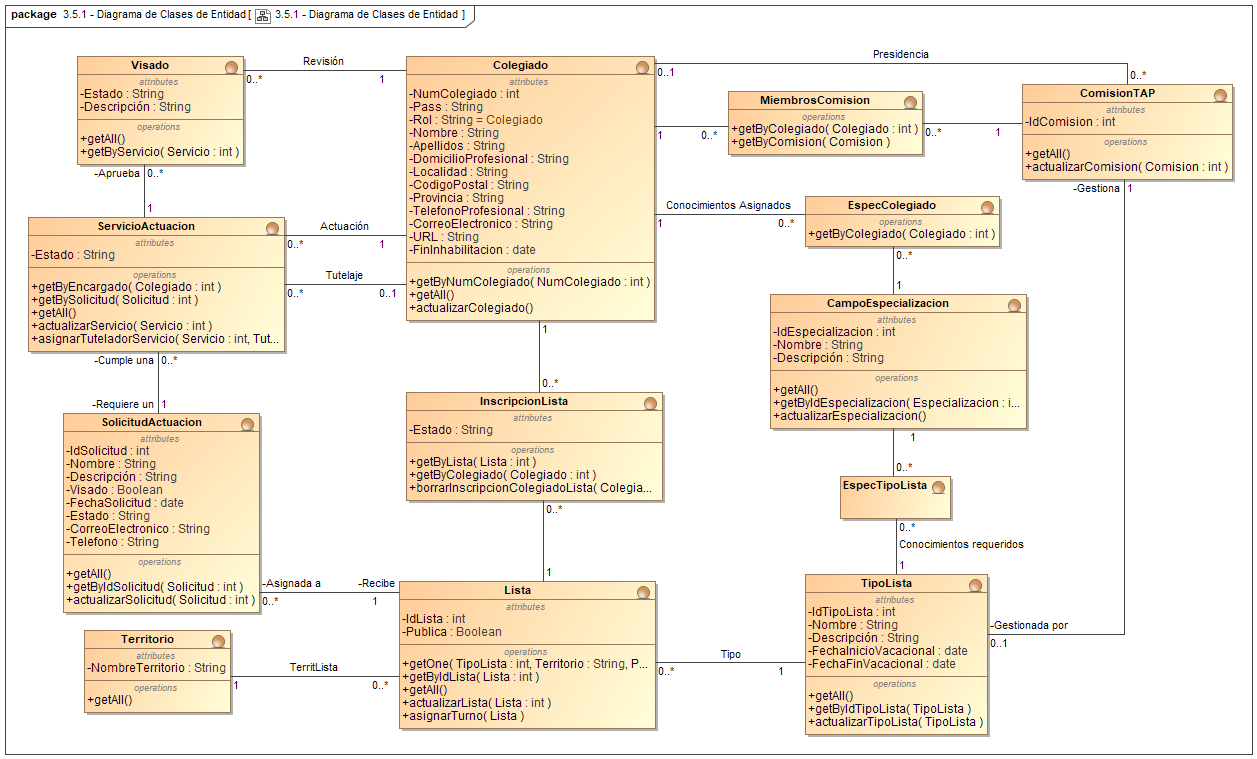
\includegraphics[width=150mm]{3_5-ClasesEntidad.png}
  \caption{Diagrama de Clases (Entidades)}
  \label{fig:ClasesEntidad}
\end{figure}
\FloatBarrier

\addtocounter{figura}{1}
Después tenemos el diagrama de clases de interfaz (\textbf{\hyperref[fig:ClasesInterfaz]{Figura \arabic{figura}}}), que establece las vistas que contendrá la aplicación a desarrollar. Estos objetos cuentan con operaciones que podrá realizar el usuario sobre cada vista, haciendo referencia en su mayoría a los botones de las mismas.
\begin{figure}[!htbp]
  \centering
  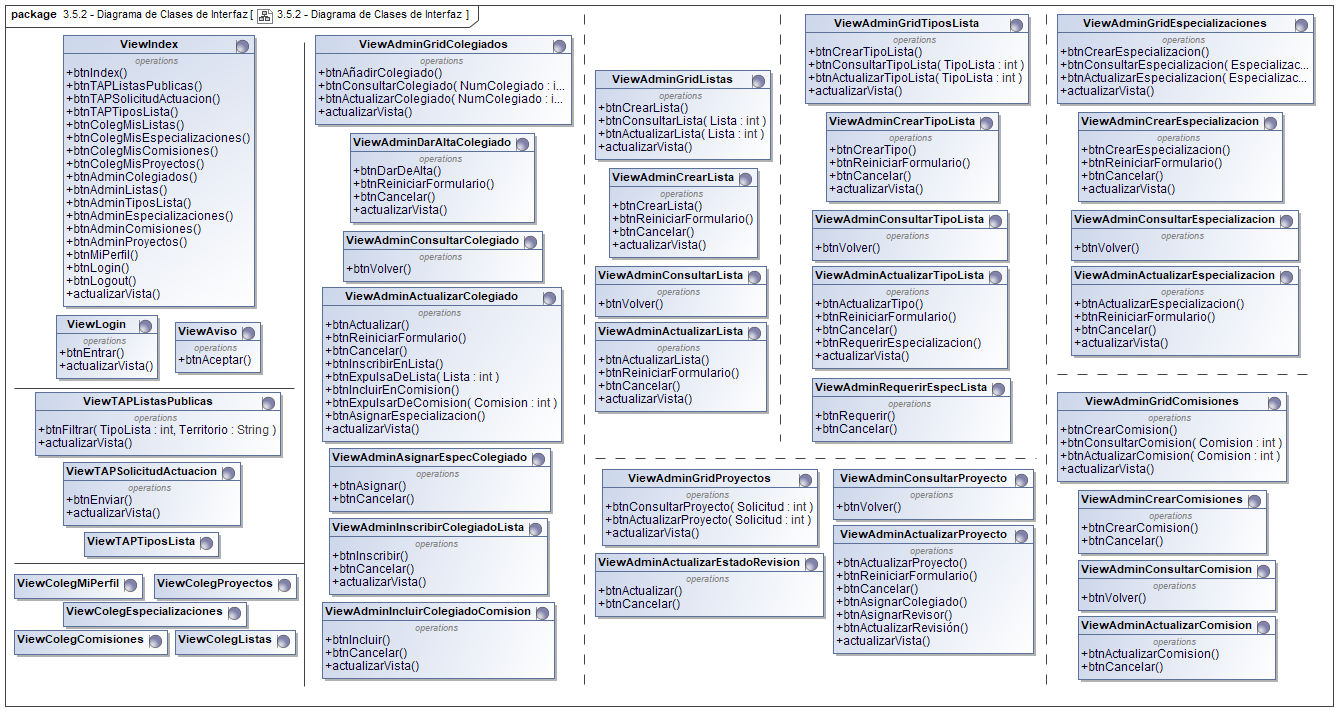
\includegraphics[width=150mm]{3_5-ClasesInterfaz.png}
  \caption{Diagrama de Clases (Interfaces)}
  \label{fig:ClasesInterfaz}
\end{figure}
\FloatBarrier

\addtocounter{figura}{1}
Por último tenemos el diagrama de clases de control (\textbf{\hyperref[fig:ClasesControl]{Figura \arabic{figura}}}), que se encarga de actuar entre las entidades y las interfaces. Estas son las que realizan en su mayoría la actividad del sistema.
\begin{figure}[!htbp]
  \centering
  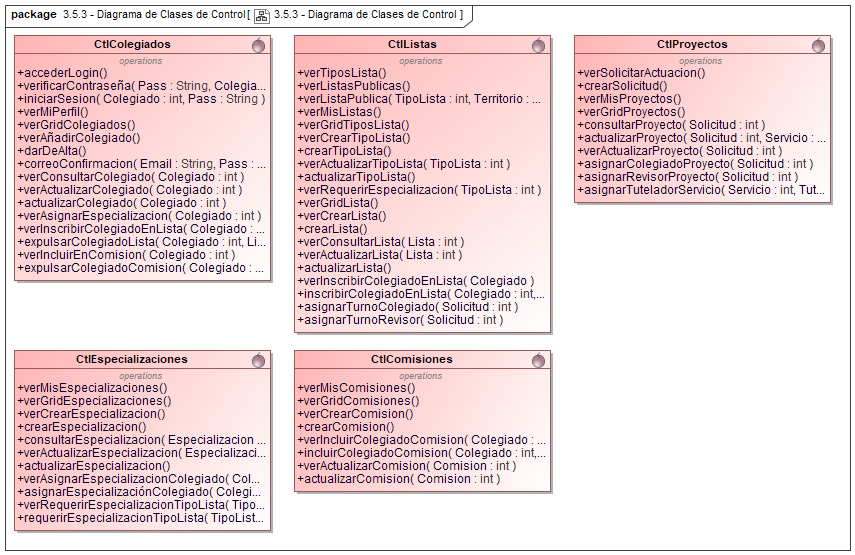
\includegraphics[width=150mm]{3_5-ClasesControl.png}
  \caption{Diagrama de Clases (Control)}
  \label{fig:ClasesControl}
\end{figure}
\FloatBarrier


\pagebreak
\section{Diagramas de Secuencia}
Los diagramas de secuencia sirven para describir el comportamiento dinámico del sistema, haciendo énfasis en la secuencia de mensajes intercambiados por los objetos. Estos describirán el flujo normal y alternativo definido en los \textbf{\hyperref[cu]{Casos de Uso}} utilizando los objetos de los diagramas de clases del apartado \textbf{\hyperref[mc]{Modelo de Clases}}.


\addtocounter{figura}{1}
Primero, respecto al caso de uso \textbf{\hyperref[tab:cuuConsultaTiposLst]{Consultar Tipos de Lista (CU01)}}, tenemos el diagrama de secuencia del flujo normal (\textbf{\hyperref[fig:Secuencia_CU1_Normal]{Figura \arabic{figura}}}).
\begin{figure}[!htbp]
  \centering
  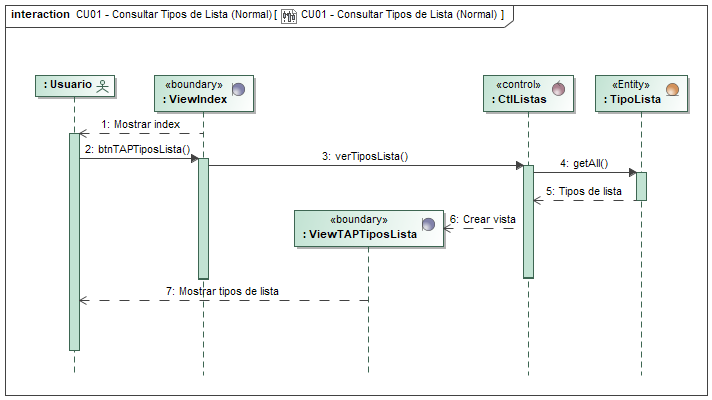
\includegraphics[width=150mm]{DiagramasSecuencia/CU01_Normal.png}
  \caption{Diagrama de Secuencia (Caso de Uso 1 - Flujo Normal)}
  \label{fig:Secuencia_CU1_Normal}
\end{figure}
\FloatBarrier

\addtocounter{figura}{1}
Después, respecto al caso de uso \textbf{\hyperref[tab:cuuConsultaLstPub]{Consultar Lista Pública (CU02)}}, tenemos el flujo de secuencia normal (\textbf{\hyperref[fig:Secuencia_CU2_Normal]{Figura \arabic{figura}}}).
\begin{figure}[!htbp]
  \centering
  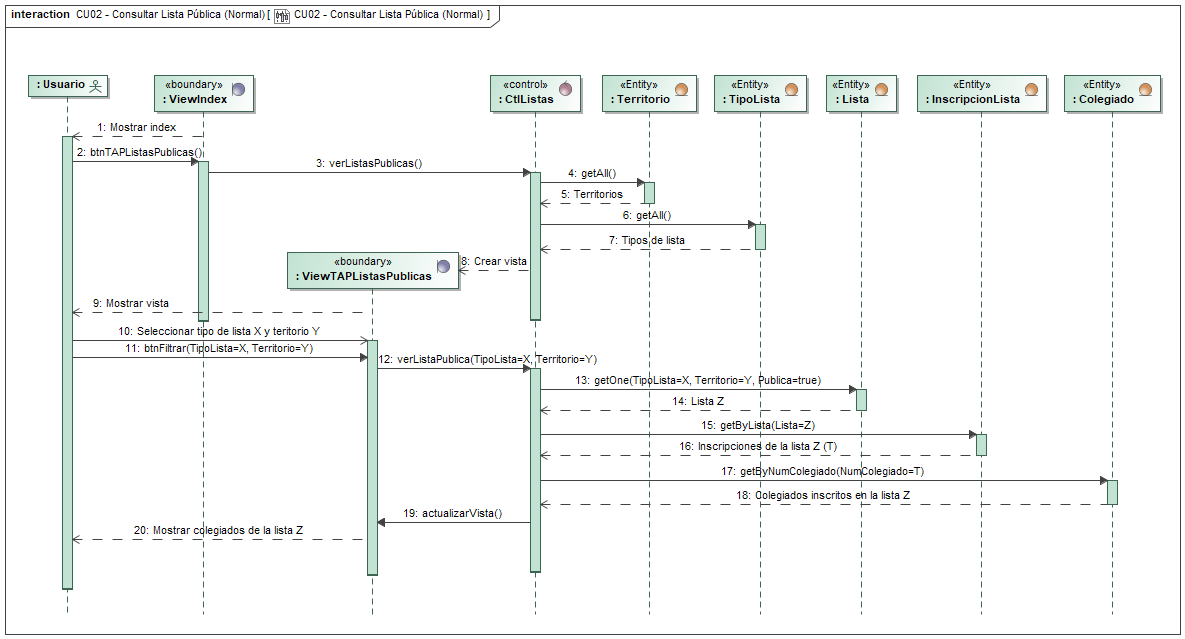
\includegraphics[width=150mm]{DiagramasSecuencia/CU02_Normal.png}
  \caption{Diagrama de Secuencia (Caso de Uso 2 - Flujo Normal)}
  \label{fig:Secuencia_CU2_Normal}
\end{figure}
\FloatBarrier

\addtocounter{figura}{1}
El tercer caso de uso, \textbf{\hyperref[tab:cuuRegPeticProf]{Registrar Petición de Profesional (CU03)}}, tiene un flujo normal y otro alternativo en caso de que no se introduzca algún valor obligatorio, definidos en la \textbf{\hyperref[fig:Secuencia_CU3_Normal]{Figura \arabic{figura}}}\addtocounter{figura}{1} y la \textbf{\hyperref[fig:Secuencia_CU3_Alt1]{Figura \arabic{figura}}} respectivamente.
\begin{figure}[!htbp]
  \centering
  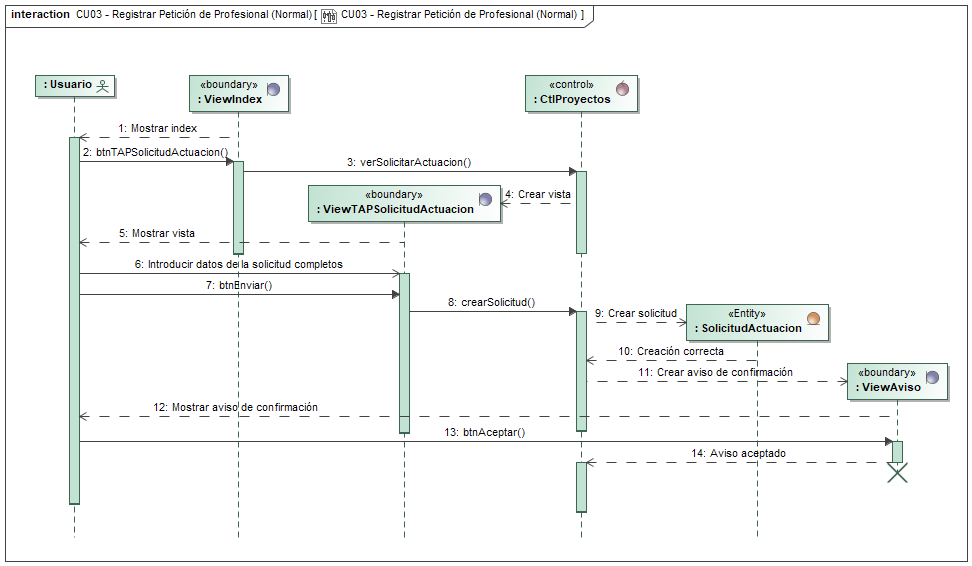
\includegraphics[width=150mm]{DiagramasSecuencia/CU03_Normal.png}
  \caption{Diagrama de Secuencia (Caso de Uso 3 - Flujo Normal)}
  \label{fig:Secuencia_CU3_Normal}
\end{figure}
\FloatBarrier

\begin{figure}[!htbp]
  \centering
  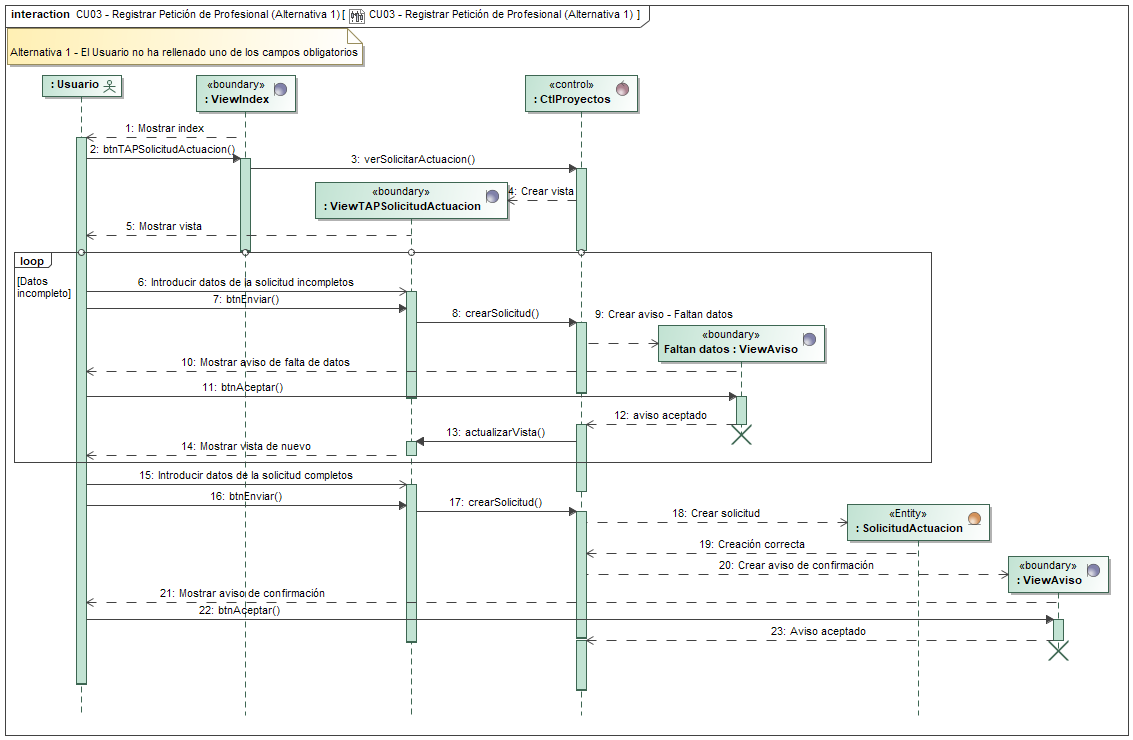
\includegraphics[width=150mm]{DiagramasSecuencia/CU03_Alt1.png}
  \caption{Diagrama de Secuencia (Caso de Uso 3 - Flujo Alternativo 1)}
  \label{fig:Secuencia_CU3_Alt1}
\end{figure}
\FloatBarrier

\addtocounter{figura}{1}
\textbf{\hyperref[tab:cucIniSes]{Iniciar Sesión (CU04)}}, tiene un flujo de secuencia normal (\textbf{\hyperref[fig:Secuencia_CU4_Normal]{Figura \arabic{figura}}}) \addtocounter{figura}{1} y uno alternativo si se introduce una contraseña equivocada (\textbf{\hyperref[fig:Secuencia_CU4_Alt1]{Figura \arabic{figura}}}).
\begin{figure}[!htbp]
  \centering
  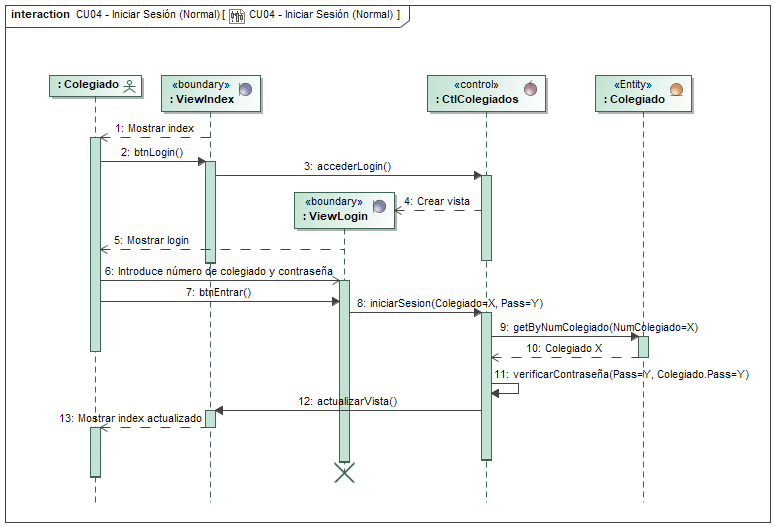
\includegraphics[width=150mm]{DiagramasSecuencia/CU04_Normal.png}
  \caption{Diagrama de Secuencia (Caso de Uso 4 - Flujo Normal)}
  \label{fig:Secuencia_CU4_Normal}
\end{figure}
\FloatBarrier

\begin{figure}[!htbp]
  \centering
  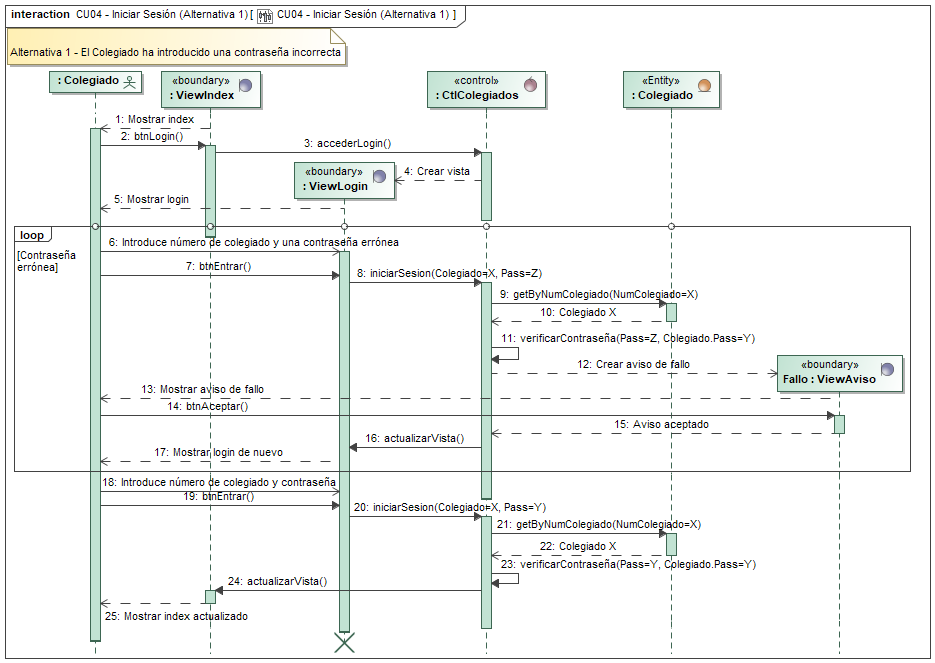
\includegraphics[width=150mm]{DiagramasSecuencia/CU04_Alt1.png}
  \caption{Diagrama de Secuencia (Caso de Uso 4 - Flujo Alternativo 1)}
  \label{fig:Secuencia_CU4_Alt1}
\end{figure}
\FloatBarrier

\addtocounter{figura}{1}
El caso de uso \textbf{\hyperref[tab:cucConsultaInfoPersonal]{Consultar Información Personal (CU05)}}, tiene únicamente un flujo de secuencia normal (\textbf{\hyperref[fig:Secuencia_CU5_Normal]{Figura \arabic{figura}}}).
\begin{figure}[!htbp]
  \centering
  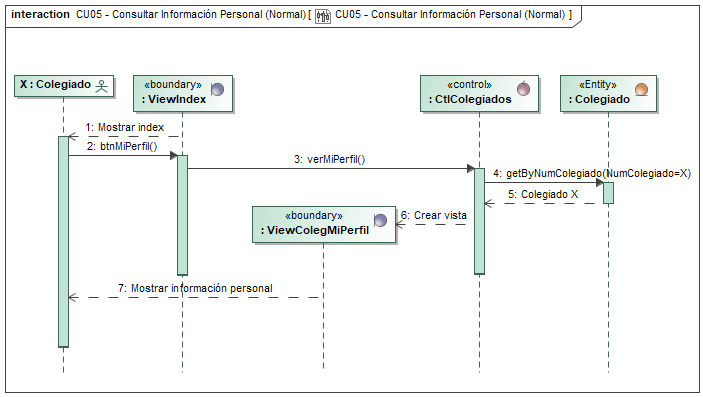
\includegraphics[width=150mm]{DiagramasSecuencia/CU05_Normal.png}
  \caption{Diagrama de Secuencia (Caso de Uso 5 - Flujo Normal)}
  \label{fig:Secuencia_CU5_Normal}
\end{figure}
\FloatBarrier

\addtocounter{figura}{1}
El caso de uso \textbf{\hyperref[tab:cucConsultaEspec]{Consultar Especializaciones Propias (CU06)}}, tiene únicamente un flujo de secuencia normal (\textbf{\hyperref[fig:Secuencia_CU6_Normal]{Figura \arabic{figura}}}).
\begin{figure}[!htbp]
  \centering
  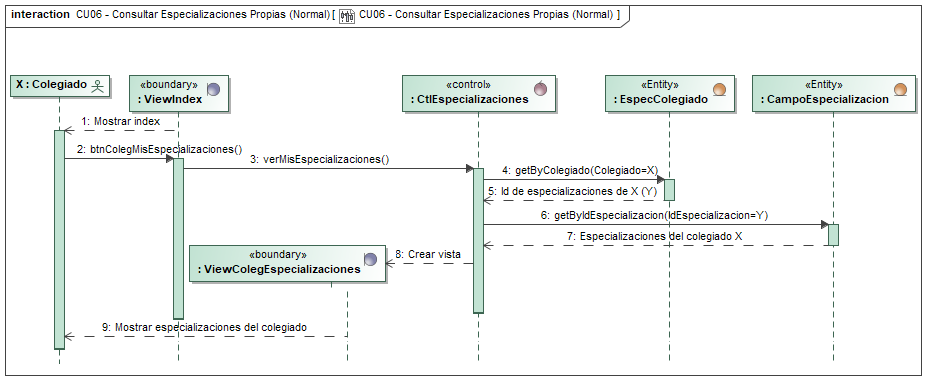
\includegraphics[width=150mm]{DiagramasSecuencia/CU06_Normal.png}
  \caption{Diagrama de Secuencia (Caso de Uso 6 - Flujo Normal)}
  \label{fig:Secuencia_CU6_Normal}
\end{figure}
\FloatBarrier

\addtocounter{figura}{1}
El caso de uso \textbf{\hyperref[tab:cucConsultaLista]{Consultar Listas Inscritas (CU07)}}, tiene únicamente un flujo de secuencia normal (\textbf{\hyperref[fig:Secuencia_CU7_Normal]{Figura \arabic{figura}}}).
\begin{figure}[!htbp]
  \centering
  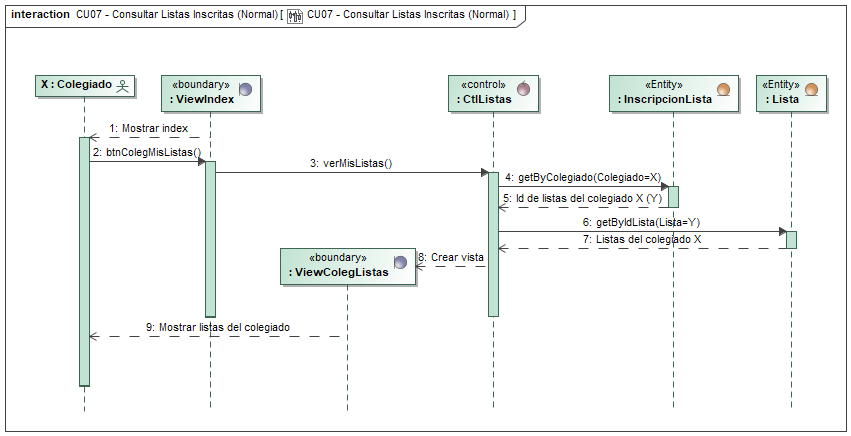
\includegraphics[width=150mm]{DiagramasSecuencia/CU07_Normal.png}
  \caption{Diagrama de Secuencia (Caso de Uso 7 - Flujo Normal)}
  \label{fig:Secuencia_CU7_Normal}
\end{figure}
\FloatBarrier

\addtocounter{figura}{1} \pagebreak
El caso de uso \textbf{\hyperref[tab:cucConsultaComision]{Consultar Participación en Comisiones (CU08)}}, tiene únicamente un flujo de secuencia normal (\textbf{\hyperref[fig:Secuencia_CU8_Normal]{Figura \arabic{figura}}}).
\begin{figure}[!htbp]
  \centering
  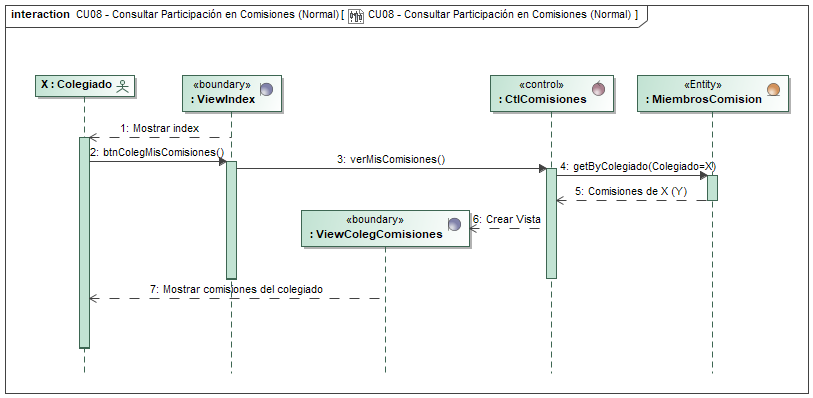
\includegraphics[width=150mm]{DiagramasSecuencia/CU08_Normal.png}
  \caption{Diagrama de Secuencia (Caso de Uso 8 - Flujo Normal)}
  \label{fig:Secuencia_CU8_Normal}
\end{figure}
\FloatBarrier

\addtocounter{figura}{1}
El caso de uso \textbf{\hyperref[tab:cucConsultaProyectos]{Consultar Participación en Proyectos (CU09)}}, tiene únicamente un flujo de secuencia normal (\textbf{\hyperref[fig:Secuencia_CU9_Normal]{Figura \arabic{figura}}}).
\begin{figure}[!htbp]
  \centering
  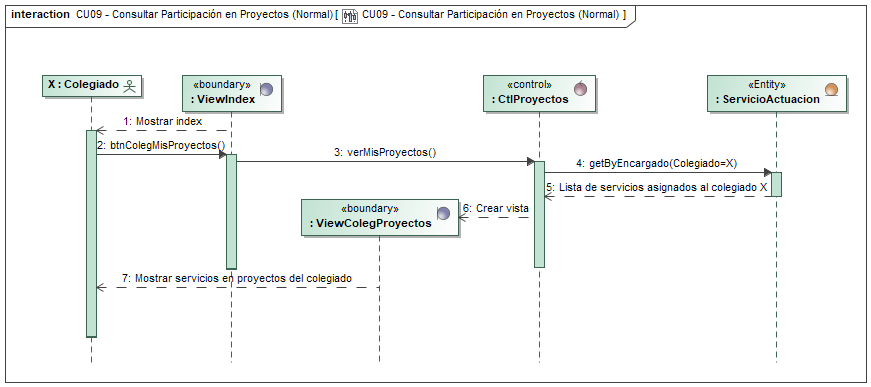
\includegraphics[width=150mm]{DiagramasSecuencia/CU09_Normal.png}
  \caption{Diagrama de Secuencia (Caso de Uso 9 - Flujo Normal)}
  \label{fig:Secuencia_CU9_Normal}
\end{figure}
\FloatBarrier

\addtocounter{figura}{1} \pagebreak
En \textbf{\hyperref[tab:curColegAlta]{Dar Alta en TAP a Colegiado (CU10)}}, tenemos un flujo de secuencia normal (\textbf{\hyperref[fig:Secuencia_CU10_Normal]{Figura \arabic{figura}}}) \addtocounter{figura}{1} y uno alternativo si se trata de introducir un número de colegiado repetido (\textbf{\hyperref[fig:Secuencia_CU10_Alt1]{Figura \arabic{figura}}}).
\begin{figure}[!htbp]
  \centering
  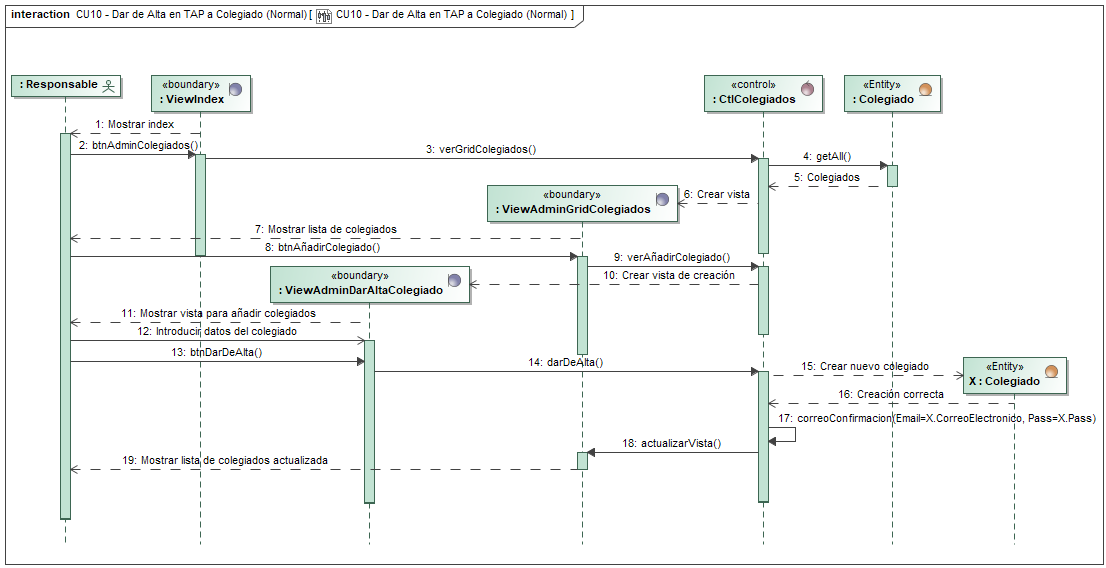
\includegraphics[width=150mm]{DiagramasSecuencia/CU10_Normal.png}
  \caption{Diagrama de Secuencia (Caso de Uso 10 - Flujo Normal)}
  \label{fig:Secuencia_CU10_Normal}
\end{figure}
\FloatBarrier

\begin{figure}[!htbp]
  \centering
  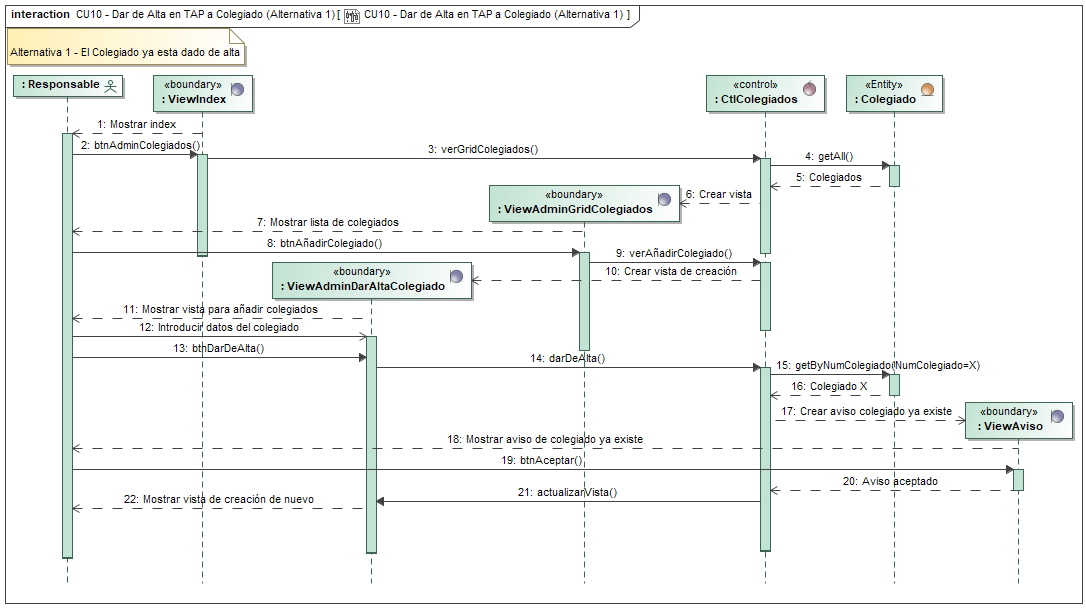
\includegraphics[width=150mm]{DiagramasSecuencia/CU10_Alt1.png}
  \caption{Diagrama de Secuencia (Caso de Uso 10 - Flujo Alternativo 1)}
  \label{fig:Secuencia_CU10_Alt1}
\end{figure}
\FloatBarrier

\addtocounter{figura}{1} \pagebreak
El caso de uso \textbf{\hyperref[tab:curConsultaInfoColeg]{Consultar Información de Colegiado (CU11)}}, tiene únicamente un flujo de secuencia normal (\textbf{\hyperref[fig:Secuencia_CU11_Normal]{Figura \arabic{figura}}}).
\begin{figure}[!htbp]
  \centering
  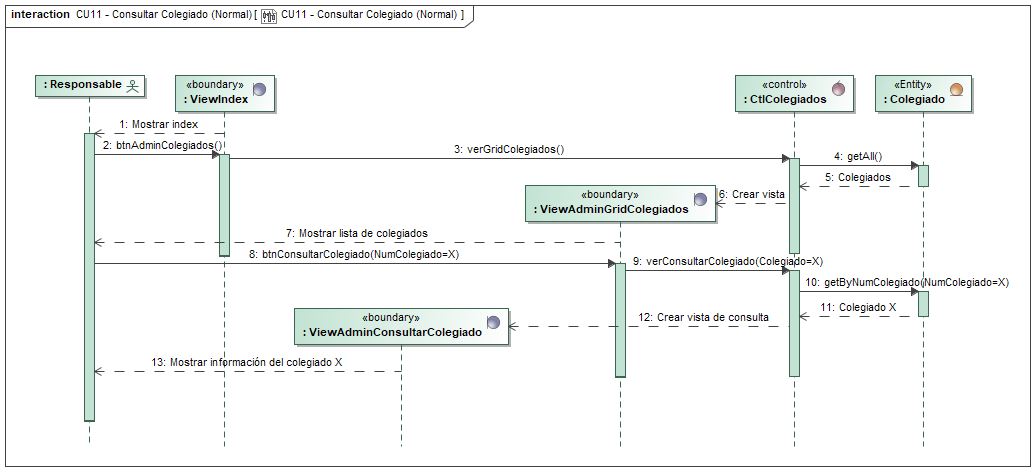
\includegraphics[width=150mm]{DiagramasSecuencia/CU11_Normal.png}
  \caption{Diagrama de Secuencia (Caso de Uso 11 - Flujo Normal)}
  \label{fig:Secuencia_CU11_Normal}
\end{figure}
\FloatBarrier

\addtocounter{figura}{1}
En \textbf{\hyperref[tab:curActualizarColeg]{Actualizar Información de un Colegiado (CU12)}}, tenemos un flujo de secuencia normal (\textbf{\hyperref[fig:Secuencia_CU12_Normal]{Figura \arabic{figura}}}) \addtocounter{figura}{1} y uno alternativo si se trata de dejar vacío un campo de datos obligatorio (\textbf{\hyperref[fig:Secuencia_CU12_Alt1]{Figura \arabic{figura}}}).
\begin{figure}[!htbp]
  \centering
  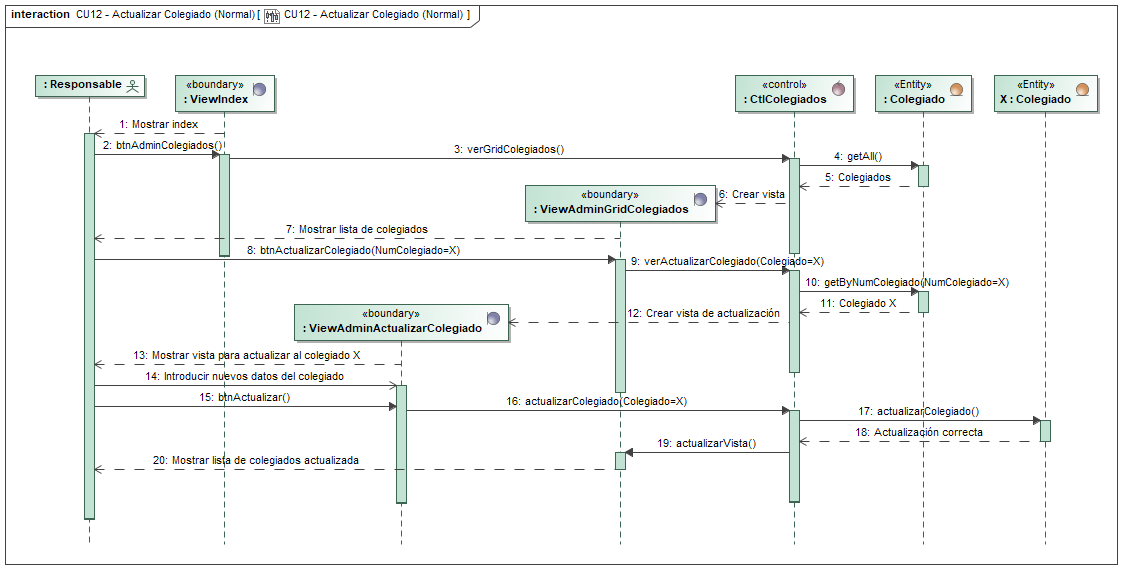
\includegraphics[width=150mm]{DiagramasSecuencia/CU12_Normal.png}
  \caption{Diagrama de Secuencia (Caso de Uso 12 - Flujo Normal)}
  \label{fig:Secuencia_CU12_Normal}
\end{figure}
\FloatBarrier

\begin{figure}[!htbp]
  \centering
  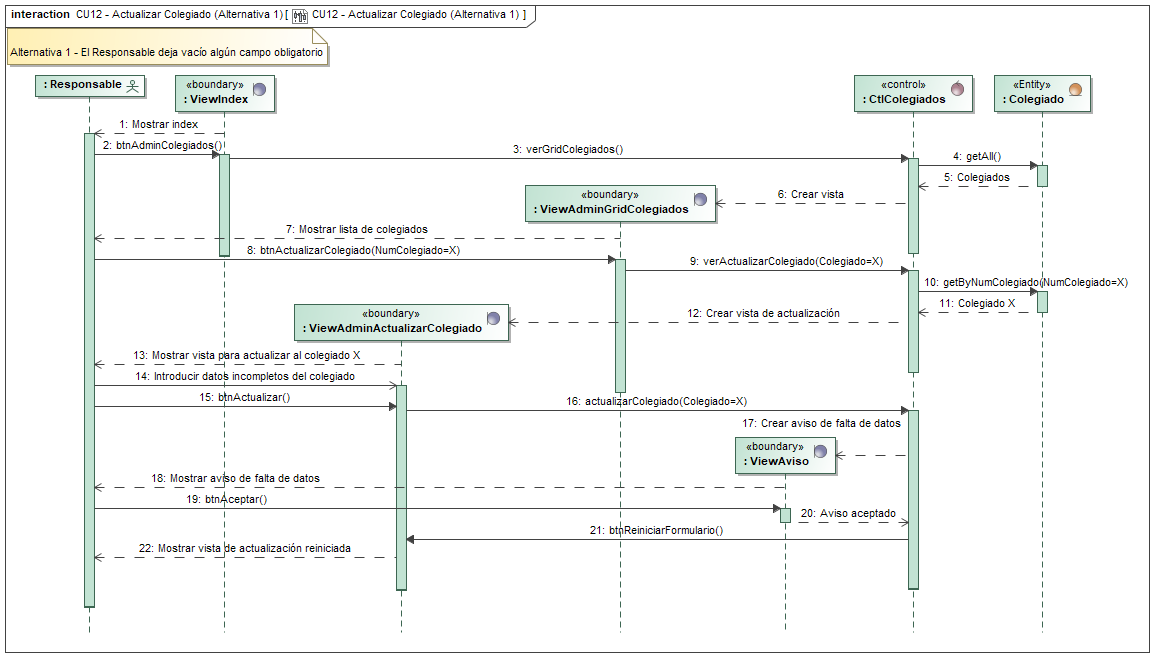
\includegraphics[width=150mm]{DiagramasSecuencia/CU12_Alt1.png}
  \caption{Diagrama de Secuencia (Caso de Uso 12 - Flujo Alternativo 1)}
  \label{fig:Secuencia_CU12_Alt1}
\end{figure}
\FloatBarrier

\addtocounter{figura}{1}
En \textbf{\hyperref[tab:curCrearTipoLst]{Crear Nuevo Tipo de Lista (CU13)}}, tenemos un flujo de secuencia normal (\textbf{\hyperref[fig:Secuencia_CU13_Normal]{Figura \arabic{figura}}}) \addtocounter{figura}{1} y uno alternativo si se trata de crear uno con un nombre ya definido para otro tipo (\textbf{\hyperref[fig:Secuencia_CU13_Alt1]{Figura \arabic{figura}}}).
\begin{figure}[!htbp]
  \centering
  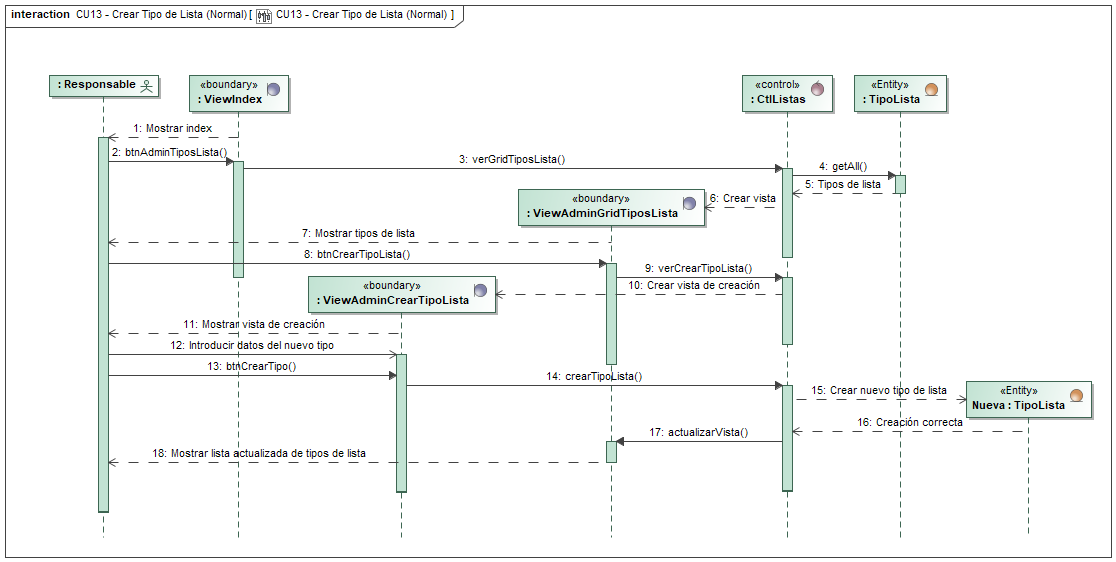
\includegraphics[width=150mm]{DiagramasSecuencia/CU13_Normal.png}
  \caption{Diagrama de Secuencia (Caso de Uso 13 - Flujo Normal)}
  \label{fig:Secuencia_CU13_Normal}
\end{figure}
\FloatBarrier

\begin{figure}[!htbp]
  \centering
  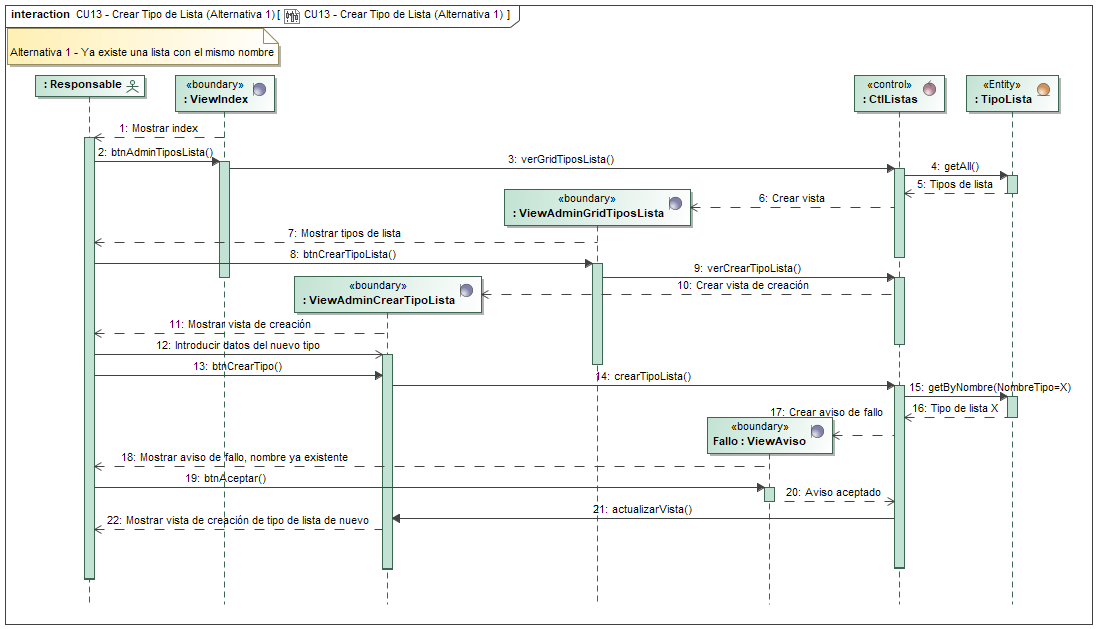
\includegraphics[width=150mm]{DiagramasSecuencia/CU13_Alt1.png}
  \caption{Diagrama de Secuencia (Caso de Uso 13 - Flujo Alternativo 1)}
  \label{fig:Secuencia_CU13_Alt1}
\end{figure}
\FloatBarrier

\addtocounter{figura}{1}
En \textbf{\hyperref[tab:curActualizarTipoLst]{Actualizar Tipo de Lista (CU14)}}, tenemos un flujo de secuencia normal (\textbf{\hyperref[fig:Secuencia_CU14_Normal]{Figura \arabic{figura}}}) \addtocounter{figura}{1} y uno alternativo si se trata de dejar vacío un campo de datos obligatorio (\textbf{\hyperref[fig:Secuencia_CU14_Alt1]{Figura \arabic{figura}}}).
\begin{figure}[!htbp]
  \centering
  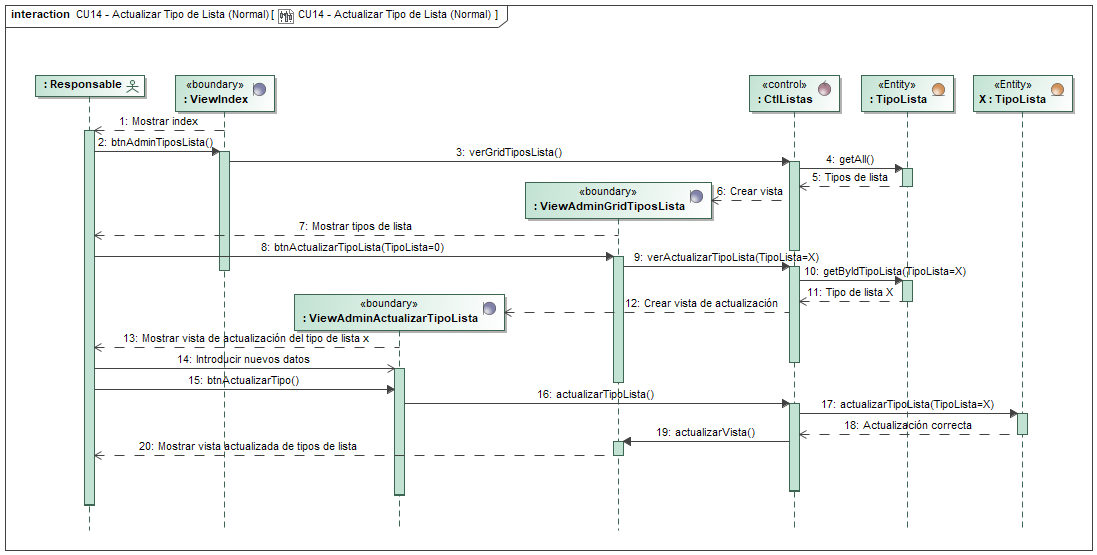
\includegraphics[width=150mm]{DiagramasSecuencia/CU14_Normal.png}
  \caption{Diagrama de Secuencia (Caso de Uso 14 - Flujo Normal)}
  \label{fig:Secuencia_CU14_Normal}
\end{figure}
\FloatBarrier

\begin{figure}[!htbp]
  \centering
  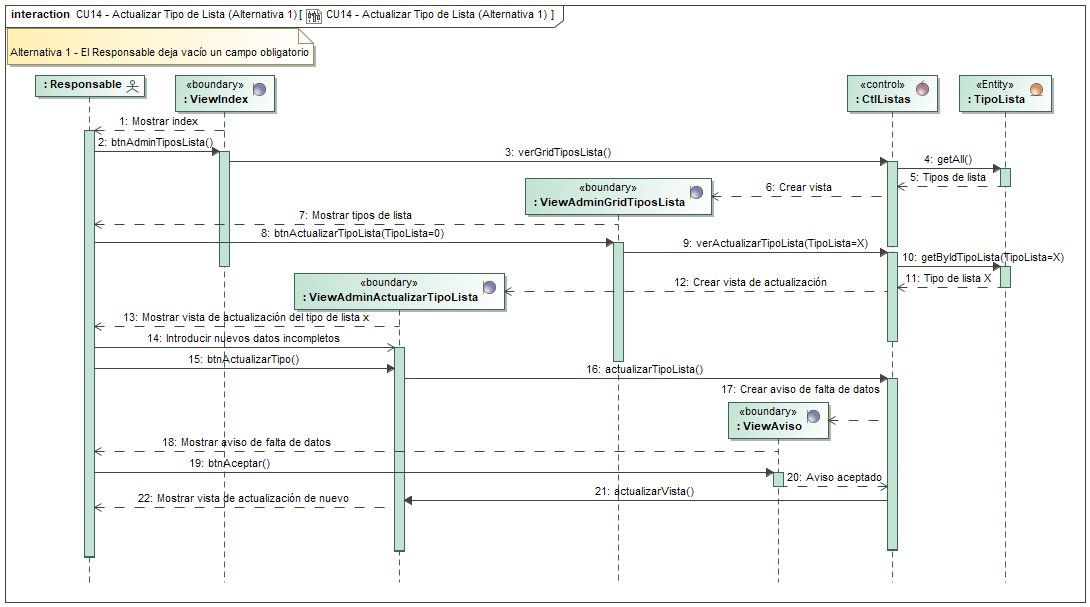
\includegraphics[width=150mm]{DiagramasSecuencia/CU14_Alt1.png}
  \caption{Diagrama de Secuencia (Caso de Uso 14 - Flujo Alternativo 1)}
  \label{fig:Secuencia_CU14_Alt1}
\end{figure}
\FloatBarrier

\addtocounter{figura}{1}
En \textbf{\hyperref[tab:curCrearEspec]{Crear una Nueva Especialización (CU15)}}, tenemos un flujo de secuencia normal (\textbf{\hyperref[fig:Secuencia_CU15_Normal]{Figura \arabic{figura}}}) \addtocounter{figura}{1} y uno alternativo si se trata de dejar vacío un campo de datos obligatorio (\textbf{\hyperref[fig:Secuencia_CU15_Alt1]{Figura \arabic{figura}}}).
\begin{figure}[!htbp]
  \centering
  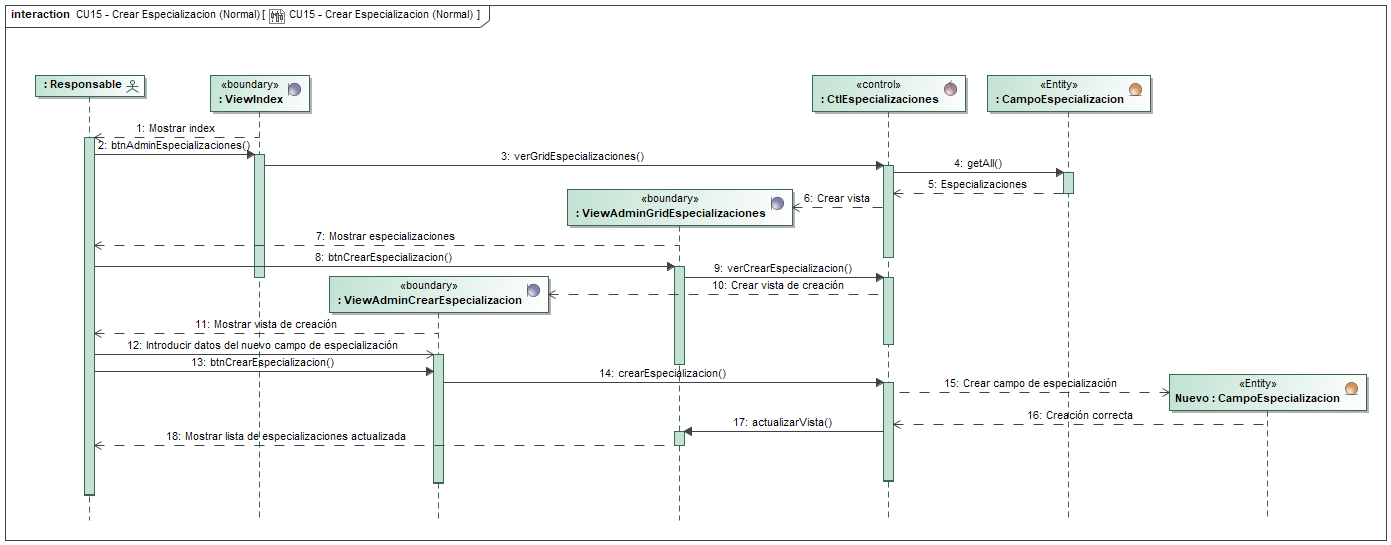
\includegraphics[width=150mm]{DiagramasSecuencia/CU15_Normal.png}
  \caption{Diagrama de Secuencia (Caso de Uso 15 - Flujo Normal)}
  \label{fig:Secuencia_CU15_Normal}
\end{figure}
\FloatBarrier

\begin{figure}[!htbp]
  \centering
  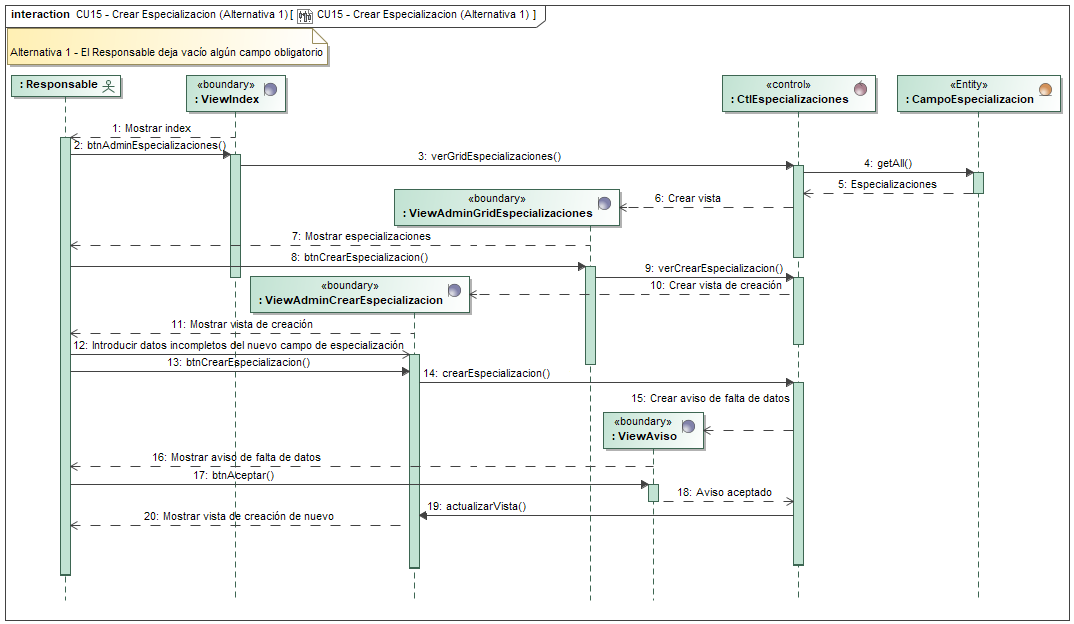
\includegraphics[width=150mm]{DiagramasSecuencia/CU15_Alt1.png}
  \caption{Diagrama de Secuencia (Caso de Uso 15 - Flujo Alternativo 1)}
  \label{fig:Secuencia_CU15_Alt1}
\end{figure}
\FloatBarrier

\addtocounter{figura}{1}
El caso de uso \textbf{\hyperref[tab:curConsultarEspec]{Consultar una Especialización (CU16)}}, tiene únicamente un flujo de secuencia normal (\textbf{\hyperref[fig:Secuencia_CU16_Normal]{Figura \arabic{figura}}}).
\begin{figure}[!htbp]
  \centering
  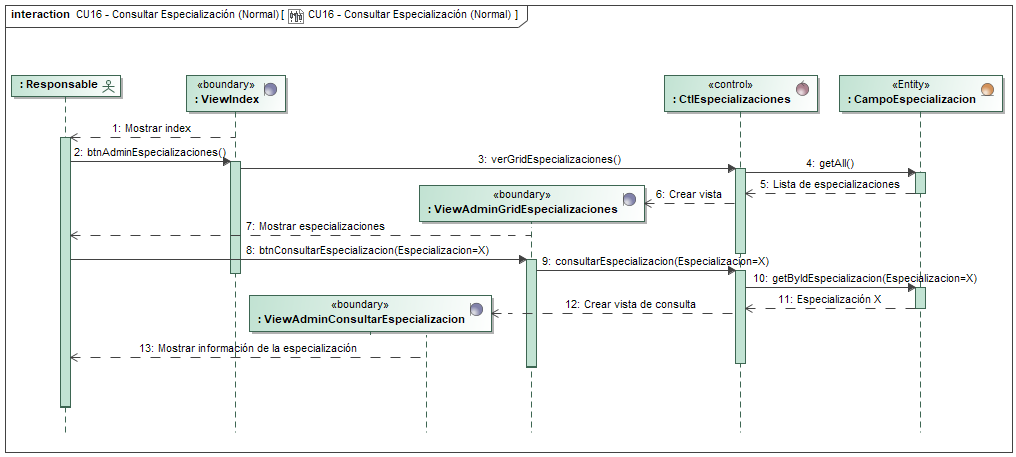
\includegraphics[width=150mm]{DiagramasSecuencia/CU16_Normal.png}
  \caption{Diagrama de Secuencia (Caso de Uso 16 - Flujo Normal)}
  \label{fig:Secuencia_CU16_Normal}
\end{figure}
\FloatBarrier

\addtocounter{figura}{1} \pagebreak
En \textbf{\hyperref[tab:curActualizarEspec]{Actualizar Información de una Especialización (CU17)}}, tenemos un flujo de secuencia normal (\textbf{\hyperref[fig:Secuencia_CU17_Normal]{Figura \arabic{figura}}}) \addtocounter{figura}{1} y uno alternativo si se trata de dejar vacío un campo de datos obligatorio (\textbf{\hyperref[fig:Secuencia_CU17_Alt1]{Figura \arabic{figura}}}).
\begin{figure}[!htbp]
  \centering
  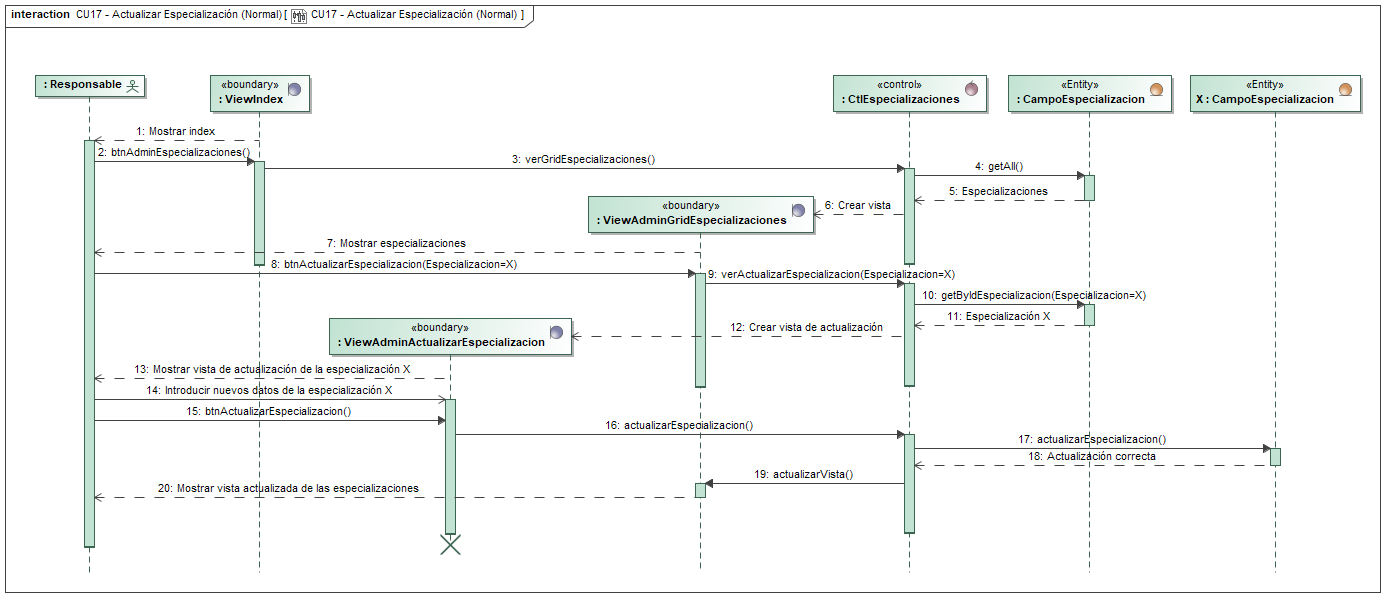
\includegraphics[width=150mm]{DiagramasSecuencia/CU17_Normal.png}
  \caption{Diagrama de Secuencia (Caso de Uso 17 - Flujo Normal)}
  \label{fig:Secuencia_CU17_Normal}
\end{figure}
\FloatBarrier

\begin{figure}[!htbp]
  \centering
  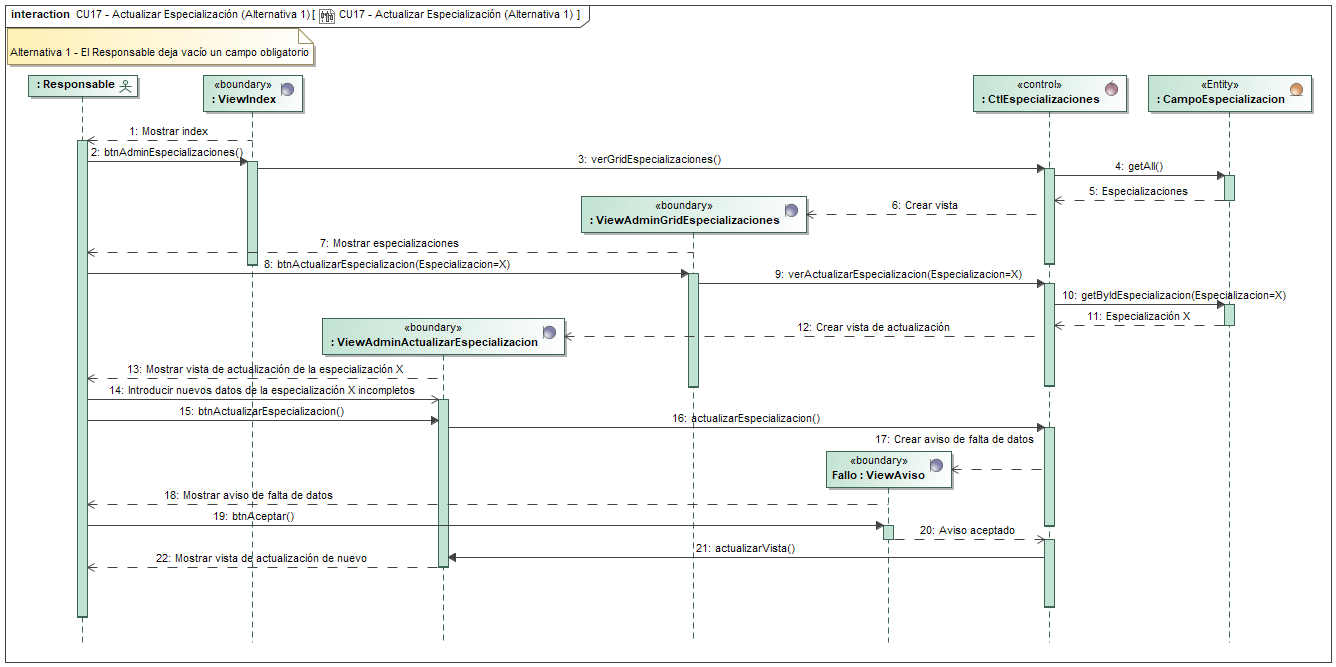
\includegraphics[width=150mm]{DiagramasSecuencia/CU17_Alt1.png}
  \caption{Diagrama de Secuencia (Caso de Uso 17 - Flujo Alternativo 1)}
  \label{fig:Secuencia_CU17_Alt1}
\end{figure}
\FloatBarrier

\addtocounter{figura}{1} \pagebreak
El caso de uso \textbf{\hyperref[tab:curAsignarEspecColeg]{Asignar Especialización a Colegiado (CU18)}}, tiene únicamente un flujo de secuencia normal (\textbf{\hyperref[fig:Secuencia_CU18_Normal]{Figura \arabic{figura}}}).
\begin{figure}[!htbp]
  \centering
  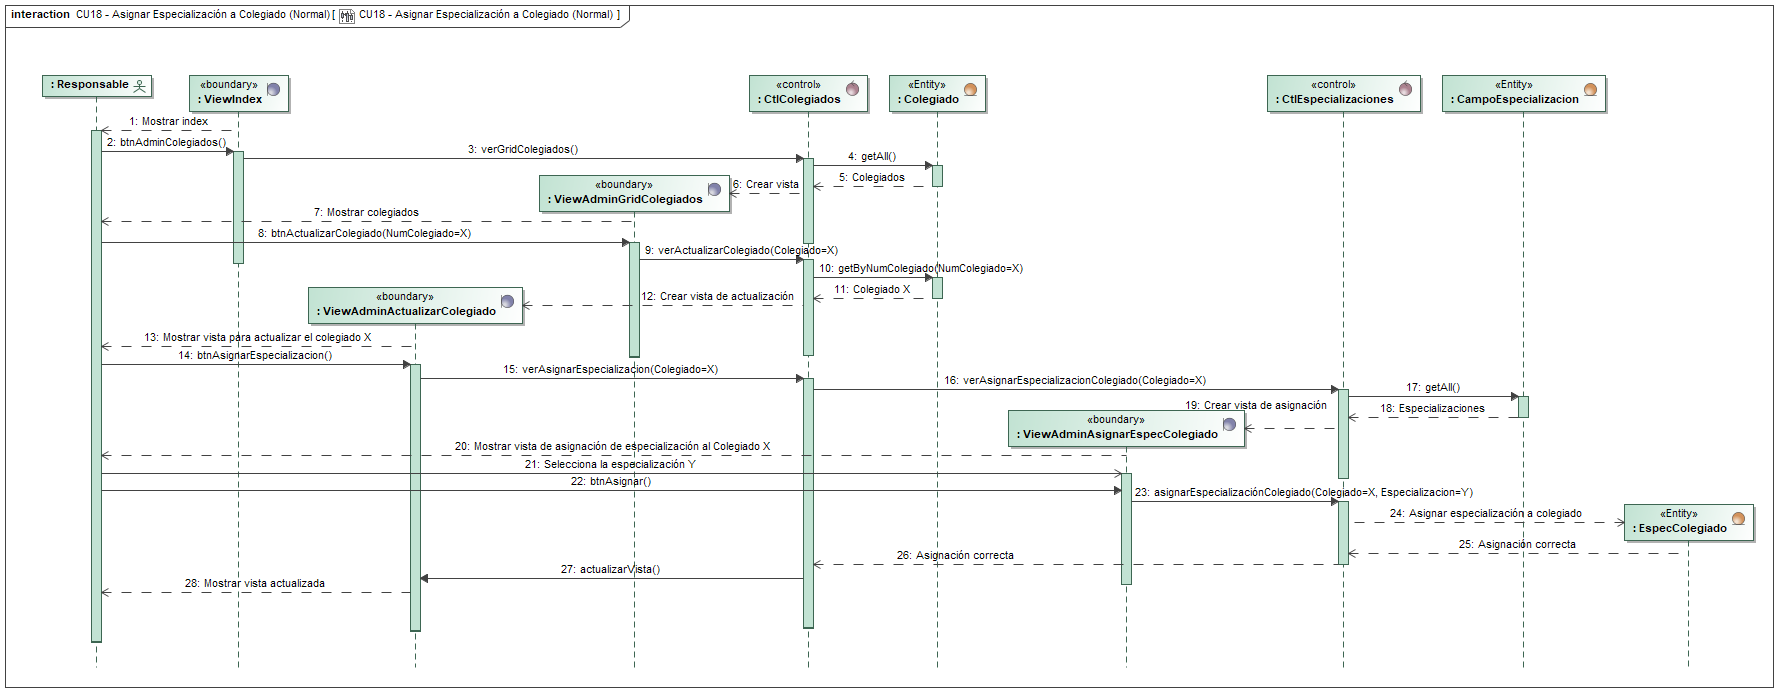
\includegraphics[width=150mm]{DiagramasSecuencia/CU18_Normal.png}
  \caption{Diagrama de Secuencia (Caso de Uso 18 - Flujo Normal)}
  \label{fig:Secuencia_CU18_Normal}
\end{figure}
\FloatBarrier

\addtocounter{figura}{1}
El caso de uso \textbf{\hyperref[tab:curRequerirEspecTipoLst]{Requerir Especialización a Tipo de Lista (CU19)}}, tiene únicamente un flujo de secuencia normal (\textbf{\hyperref[fig:Secuencia_CU19_Normal]{Figura \arabic{figura}}}).
\begin{figure}[!htbp]
  \centering
  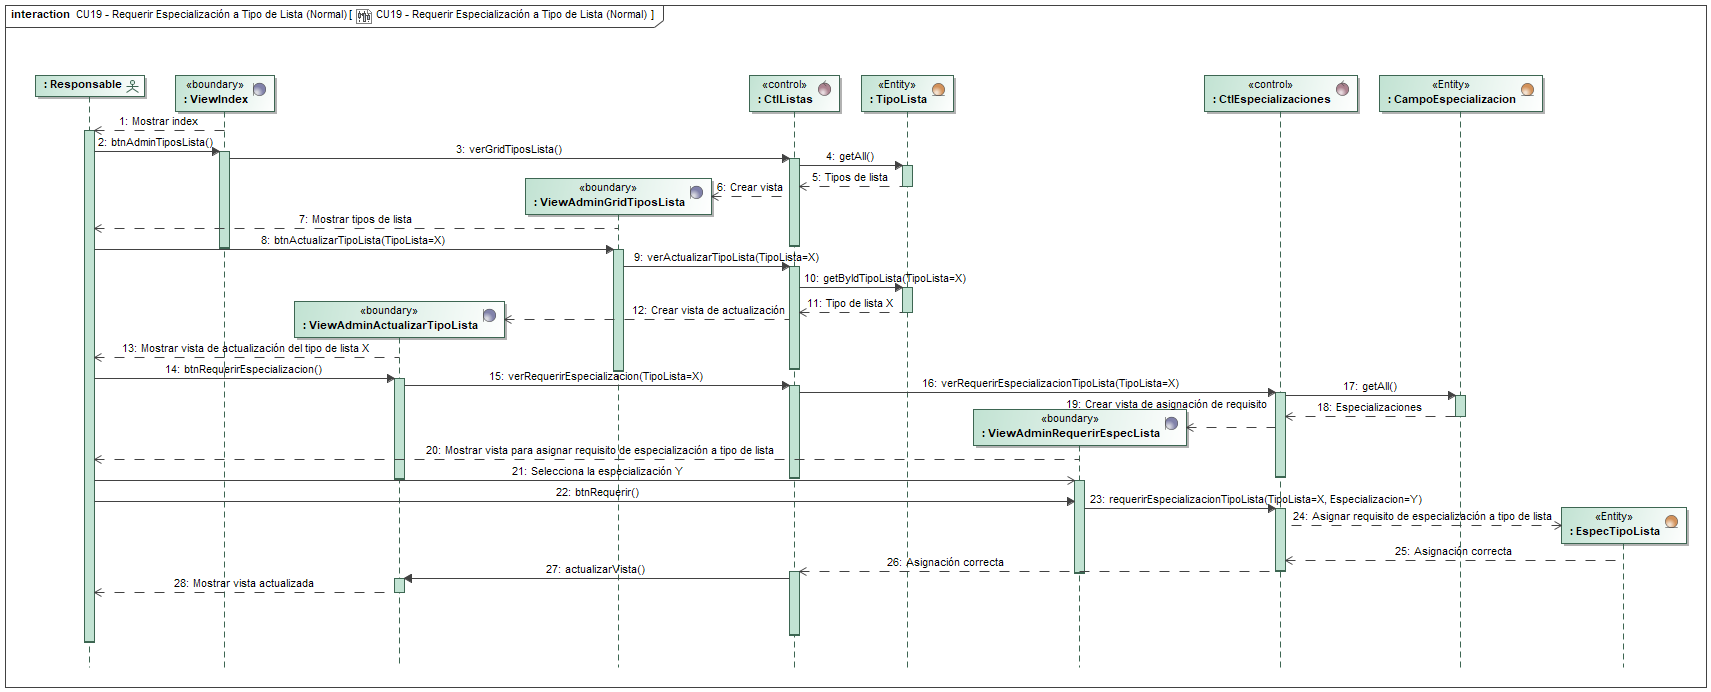
\includegraphics[width=150mm]{DiagramasSecuencia/CU19_Normal.png}
  \caption{Diagrama de Secuencia (Caso de Uso 19 - Flujo Normal)}
  \label{fig:Secuencia_CU19_Normal}
\end{figure}
\FloatBarrier

\addtocounter{figura}{1} \pagebreak
En \textbf{\hyperref[tab:curCrearLista]{Crear Lista (CU20)}}, tenemos un flujo de secuencia normal (\textbf{\hyperref[fig:Secuencia_CU20_Normal]{Figura \arabic{figura}}}) \addtocounter{figura}{1} y uno alternativo si se trata de crear una lista repetida (\textbf{\hyperref[fig:Secuencia_CU20_Alt1]{Figura \arabic{figura}}}).
\begin{figure}[!htbp]
  \centering
  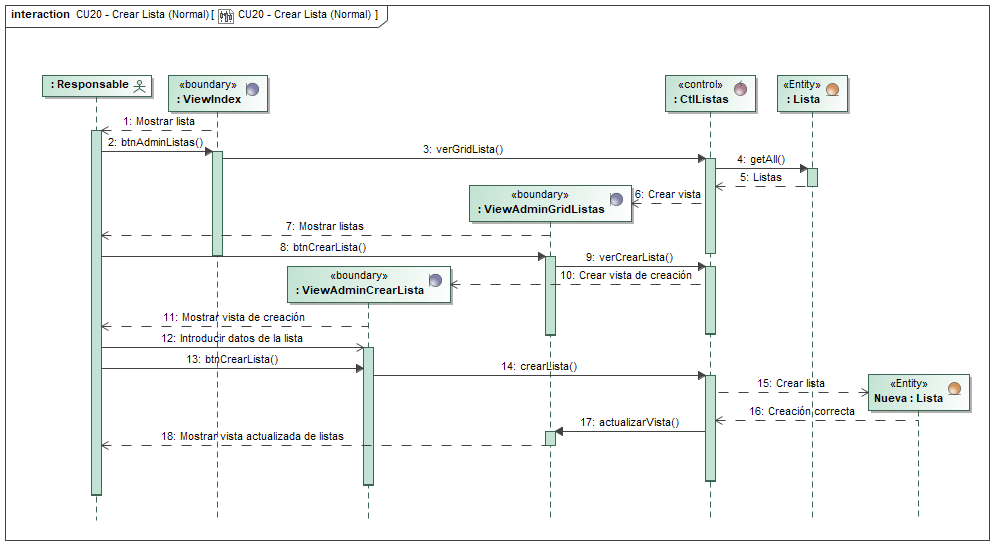
\includegraphics[width=150mm]{DiagramasSecuencia/CU20_Normal.png}
  \caption{Diagrama de Secuencia (Caso de Uso 20 - Flujo Normal)}
  \label{fig:Secuencia_CU20_Normal}
\end{figure}
\FloatBarrier

\begin{figure}[!htbp]
  \centering
  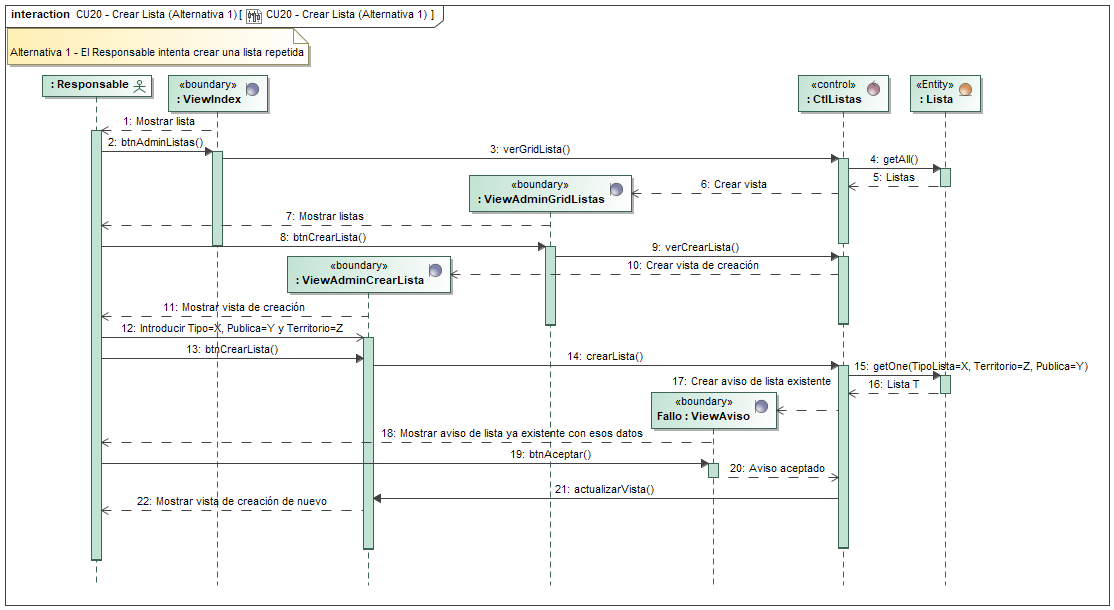
\includegraphics[width=150mm]{DiagramasSecuencia/CU20_Alt1.png}
  \caption{Diagrama de Secuencia (Caso de Uso 20 - Flujo Alternativo 1)}
  \label{fig:Secuencia_CU20_Alt1}
\end{figure}
\FloatBarrier

\addtocounter{figura}{1} \pagebreak
El caso de uso \textbf{\hyperref[tab:curConsultarLista]{Consultar Lista (CU21)}}, tiene únicamente un flujo de secuencia normal (\textbf{\hyperref[fig:Secuencia_CU21_Normal]{Figura \arabic{figura}}}).
\begin{figure}[!htbp]
  \centering
  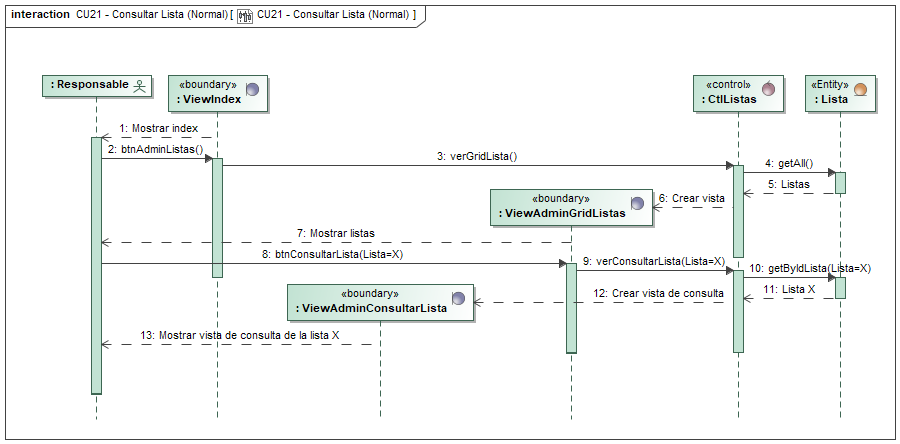
\includegraphics[width=150mm]{DiagramasSecuencia/CU21_Normal.png}
  \caption{Diagrama de Secuencia (Caso de Uso 21 - Flujo Normal)}
  \label{fig:Secuencia_CU21_Normal}
\end{figure}
\FloatBarrier

\addtocounter{figura}{1}
En \textbf{\hyperref[tab:curActualizarLista]{Actualizar Información de una Lista (CU22)}}, tenemos un flujo de secuencia normal (\textbf{\hyperref[fig:Secuencia_CU22_Normal]{Figura \arabic{figura}}}) \addtocounter{figura}{1} y uno alternativo si ya existe otra lista con los mismos datos a la que se pretende actualizar (\textbf{\hyperref[fig:Secuencia_CU22_Alt1]{Figura \arabic{figura}}}).
\begin{figure}[!htbp]
  \centering
  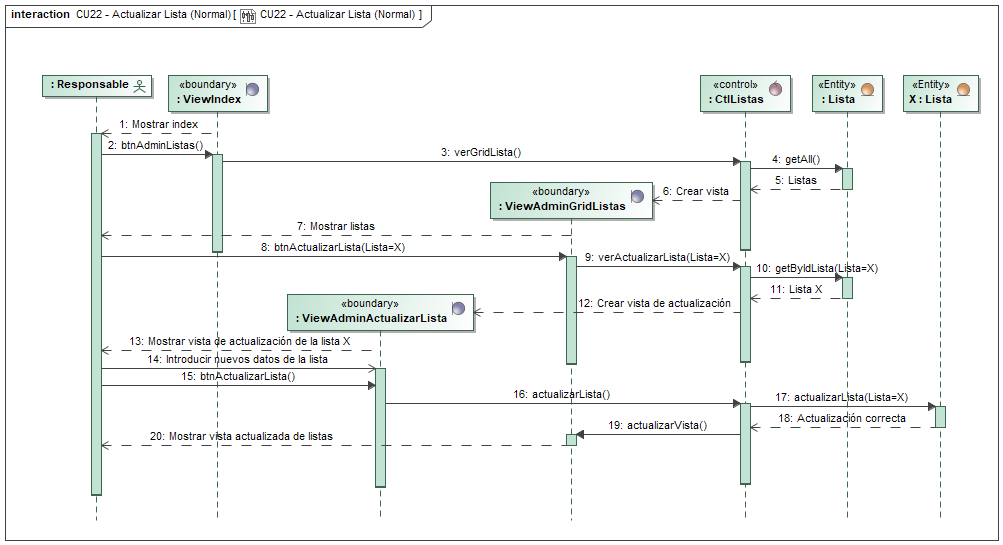
\includegraphics[width=150mm]{DiagramasSecuencia/CU22_Normal.png}
  \caption{Diagrama de Secuencia (Caso de Uso 22 - Flujo Normal)}
  \label{fig:Secuencia_CU22_Normal}
\end{figure}
\FloatBarrier

\begin{figure}[!htbp]
  \centering
  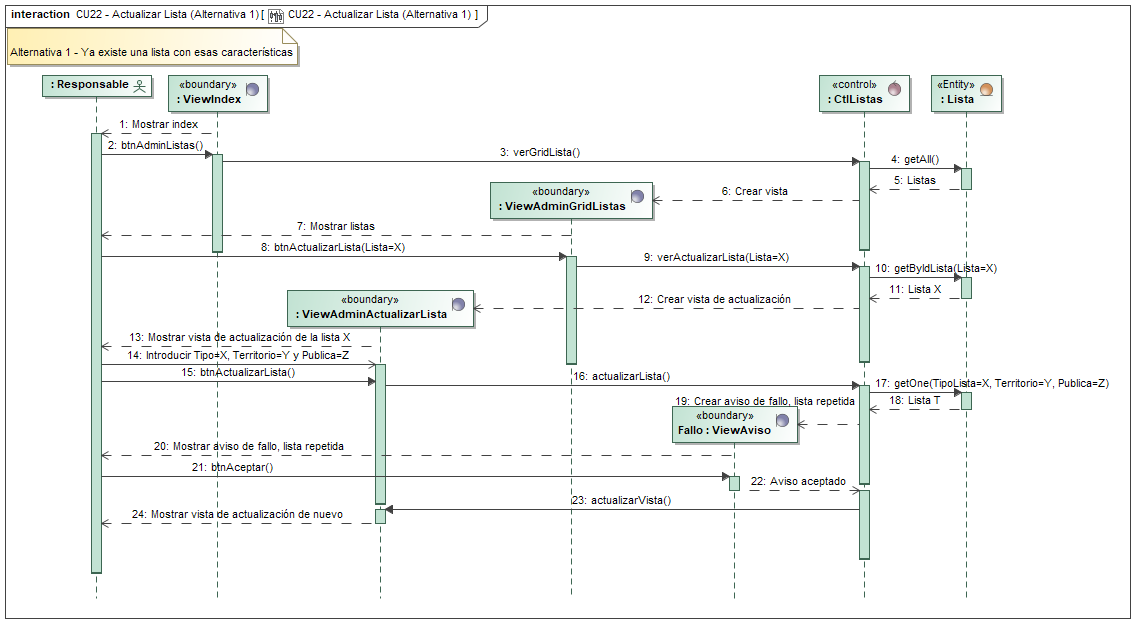
\includegraphics[width=150mm]{DiagramasSecuencia/CU22_Alt1.png}
  \caption{Diagrama de Secuencia (Caso de Uso 22 - Flujo Alternativo 1)}
  \label{fig:Secuencia_CU22_Alt1}
\end{figure}
\FloatBarrier

\addtocounter{figura}{1}
En \textbf{\hyperref[tab:curCrearInscrLst]{Añadir Inscripción a Lista (CU23)}}, tenemos un flujo de secuencia normal (\textbf{\hyperref[fig:Secuencia_CU23_Normal]{Figura \arabic{figura}}}) \addtocounter{figura}{1} y uno alternativo si el colegiado no tiene conocimientos en todas las especializaciones requeridas por la lista (\textbf{\hyperref[fig:Secuencia_CU23_Alt1]{Figura \arabic{figura}}}).
\begin{figure}[!htbp]
  \centering
  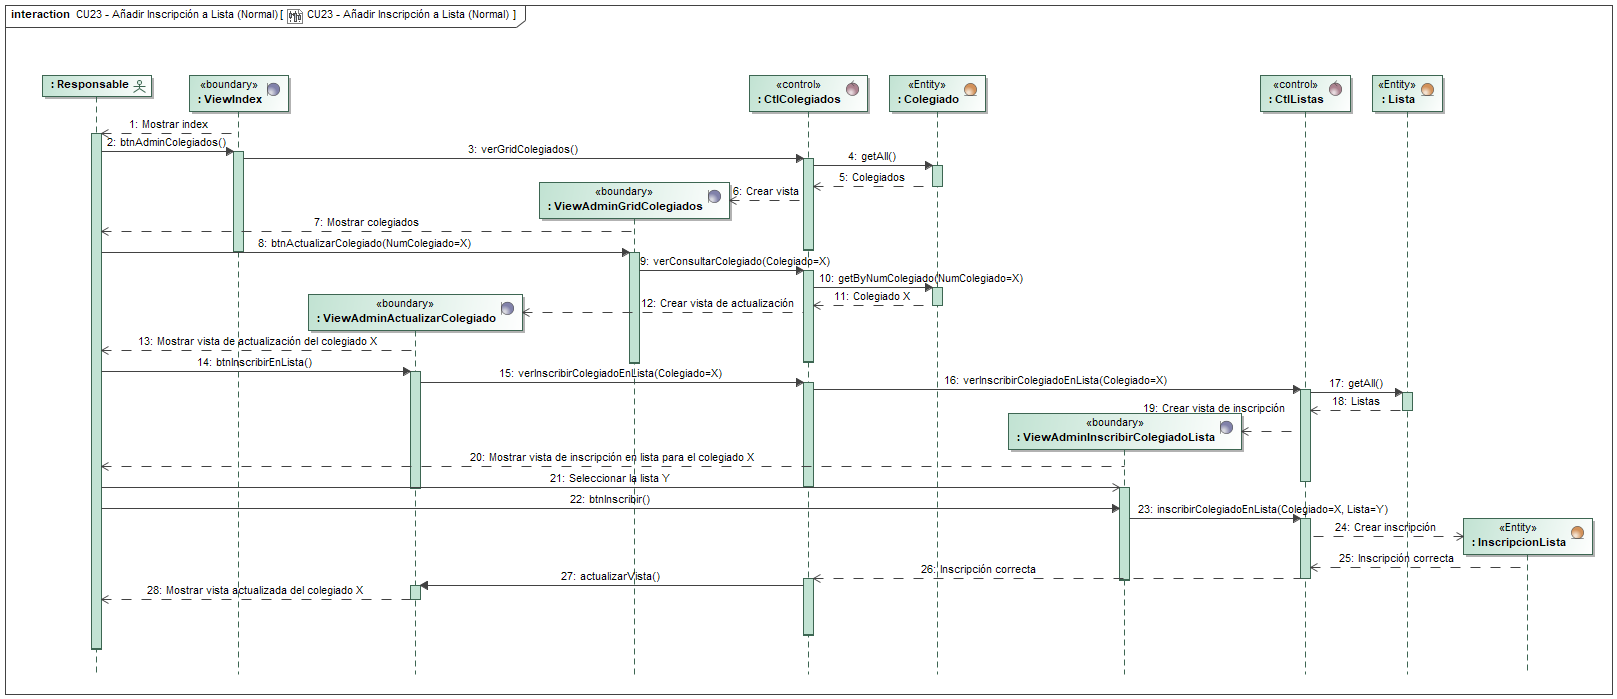
\includegraphics[width=150mm]{DiagramasSecuencia/CU23_Normal.png}
  \caption{Diagrama de Secuencia (Caso de Uso 23 - Flujo Normal)}
  \label{fig:Secuencia_CU23_Normal}
\end{figure}
\FloatBarrier

\begin{figure}[!htbp]
  \centering
  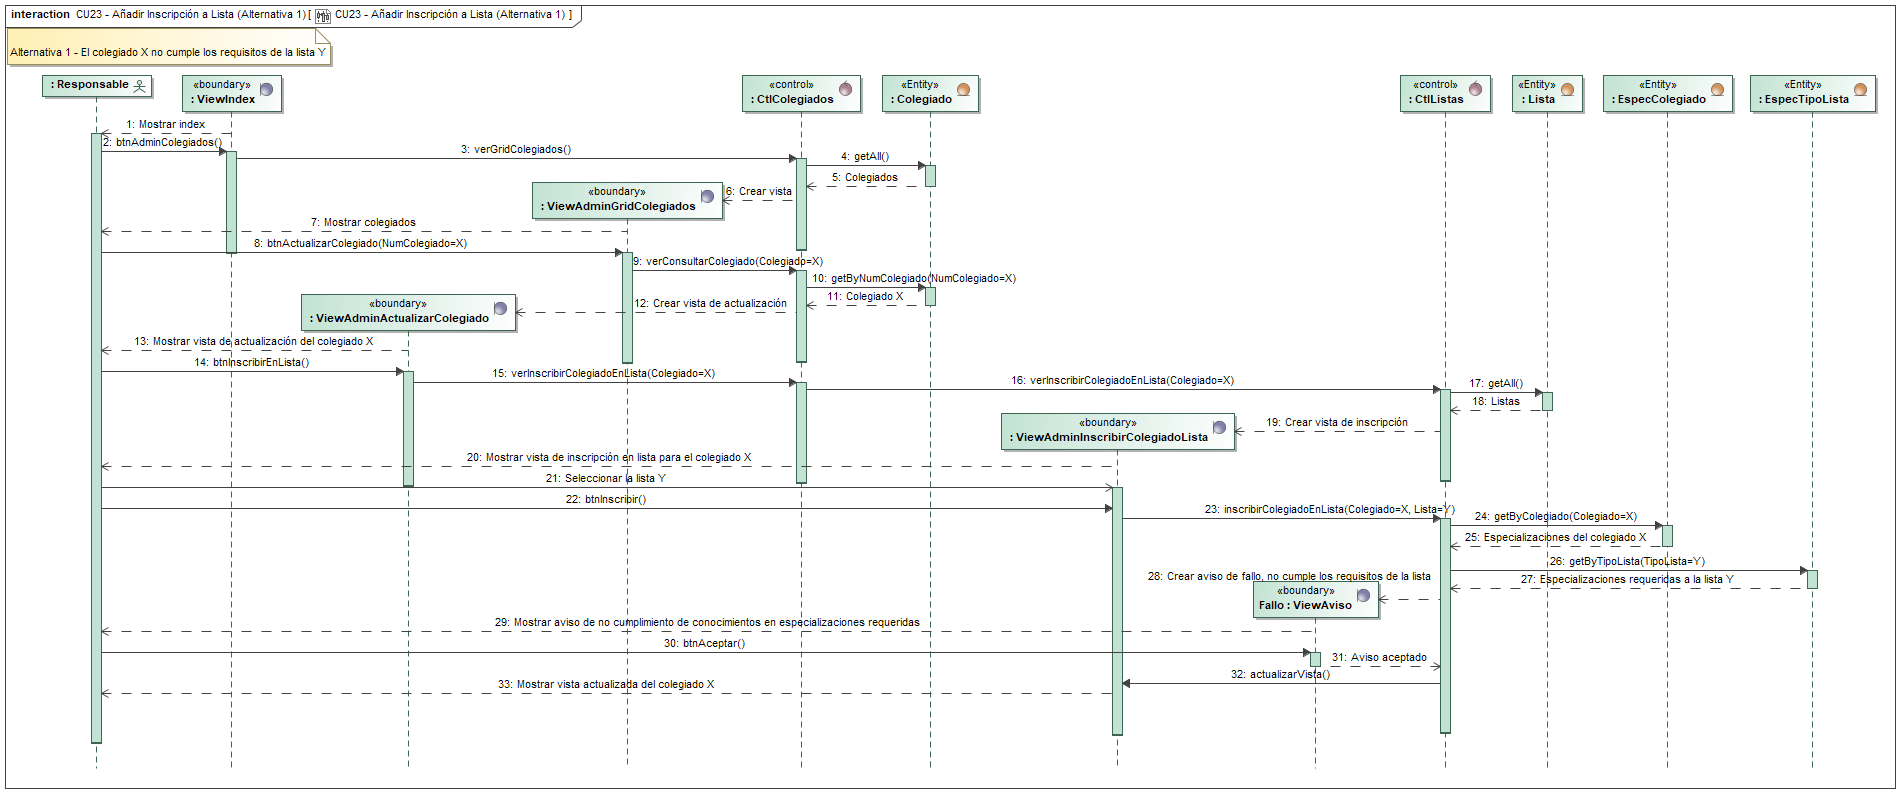
\includegraphics[width=150mm]{DiagramasSecuencia/CU23_Alt1.png}
  \caption{Diagrama de Secuencia (Caso de Uso 23 - Flujo Alternativo 1)}
  \label{fig:Secuencia_CU23_Alt1}
\end{figure}
\FloatBarrier

\addtocounter{figura}{1}
El caso de uso \textbf{\hyperref[tab:curEliminarInscrLst]{Eliminar Inscripción en Lista (CU24)}}, tiene únicamente un flujo de secuencia normal (\textbf{\hyperref[fig:Secuencia_CU24_Normal]{Figura \arabic{figura}}}).
\begin{figure}[!htbp]
  \centering
  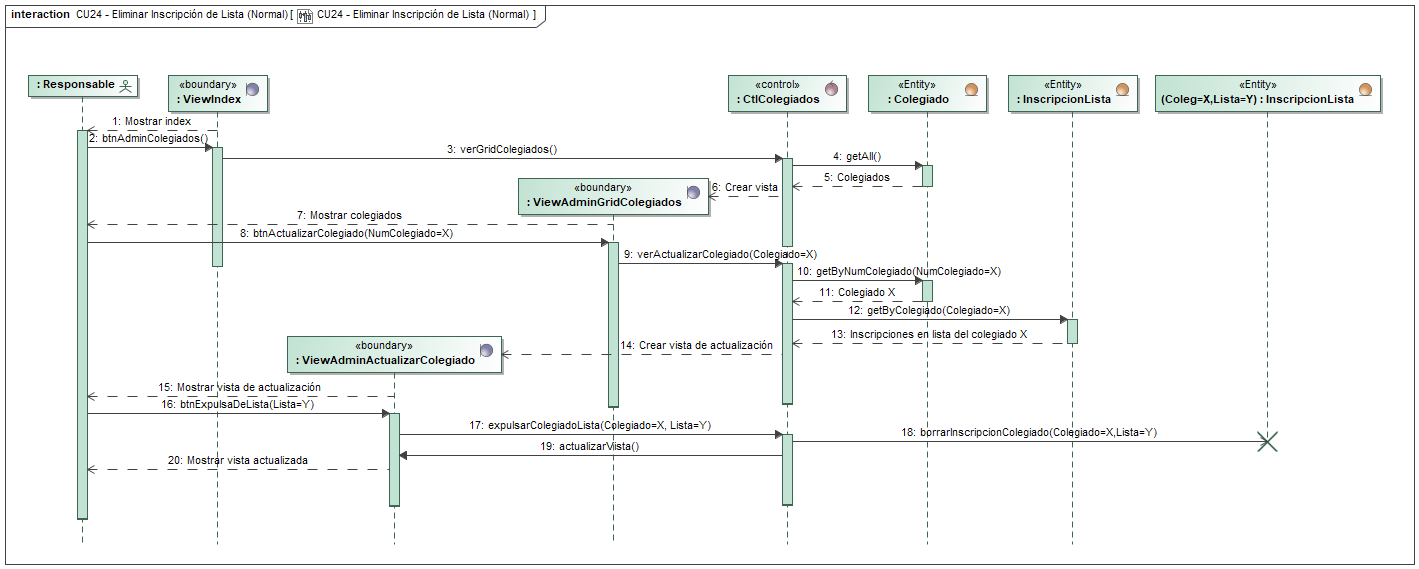
\includegraphics[width=150mm]{DiagramasSecuencia/CU24_Normal.png}
  \caption{Diagrama de Secuencia (Caso de Uso 24 - Flujo Normal)}
  \label{fig:Secuencia_CU24_Normal}
\end{figure}
\FloatBarrier

\addtocounter{figura}{1} \pagebreak
El caso de uso \textbf{\hyperref[tab:curCrearComision]{Añadir Comisión (CU25)}}, tiene únicamente un flujo de secuencia normal (\textbf{\hyperref[fig:Secuencia_CU25_Normal]{Figura \arabic{figura}}}).
\begin{figure}[!htbp]
  \centering
  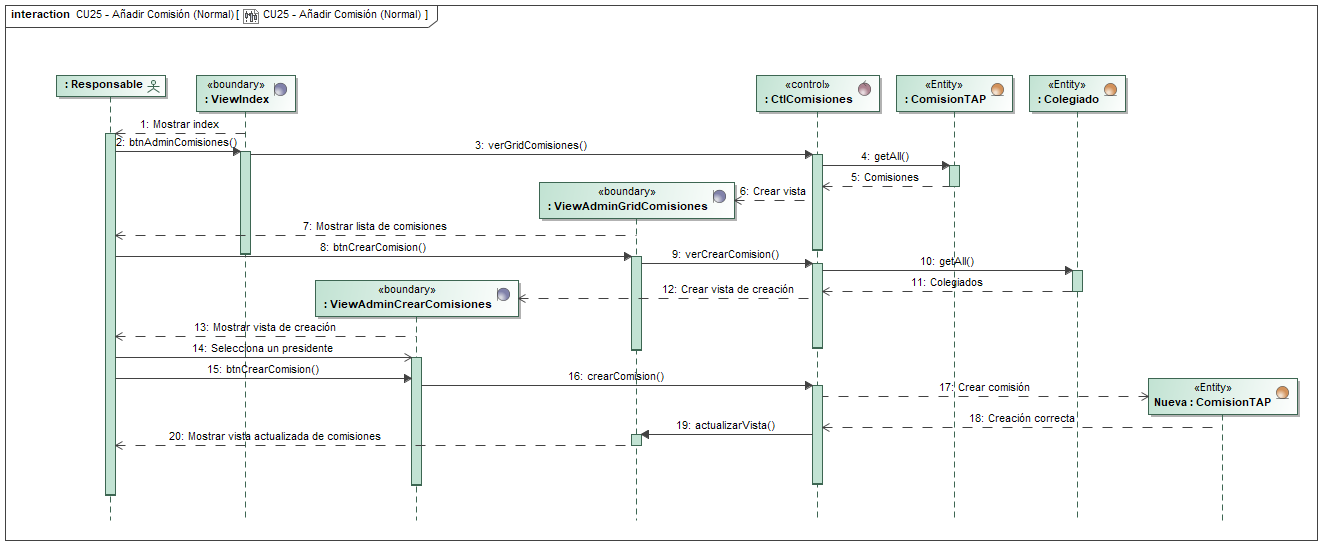
\includegraphics[width=150mm]{DiagramasSecuencia/CU25_Normal.png}
  \caption{Diagrama de Secuencia (Caso de Uso 25 - Flujo Normal)}
  \label{fig:Secuencia_CU25_Normal}
\end{figure}
\FloatBarrier

\addtocounter{figura}{1}
En \textbf{\hyperref[tab:curIncluirColegComisionTAP]{Añadir Colegiado a la Comisión de TAP (CU26)}}, tenemos un flujo de secuencia normal (\textbf{\hyperref[fig:Secuencia_CU26_Normal]{Figura \arabic{figura}}}) \addtocounter{figura}{1} y uno alternativo si el colegiado no pertenece a ninguna lista gestionada por la comisión en la que se pretende incluirle (\textbf{\hyperref[fig:Secuencia_CU26_Alt1]{Figura \arabic{figura}}}).
\begin{figure}[!htbp]
  \centering
  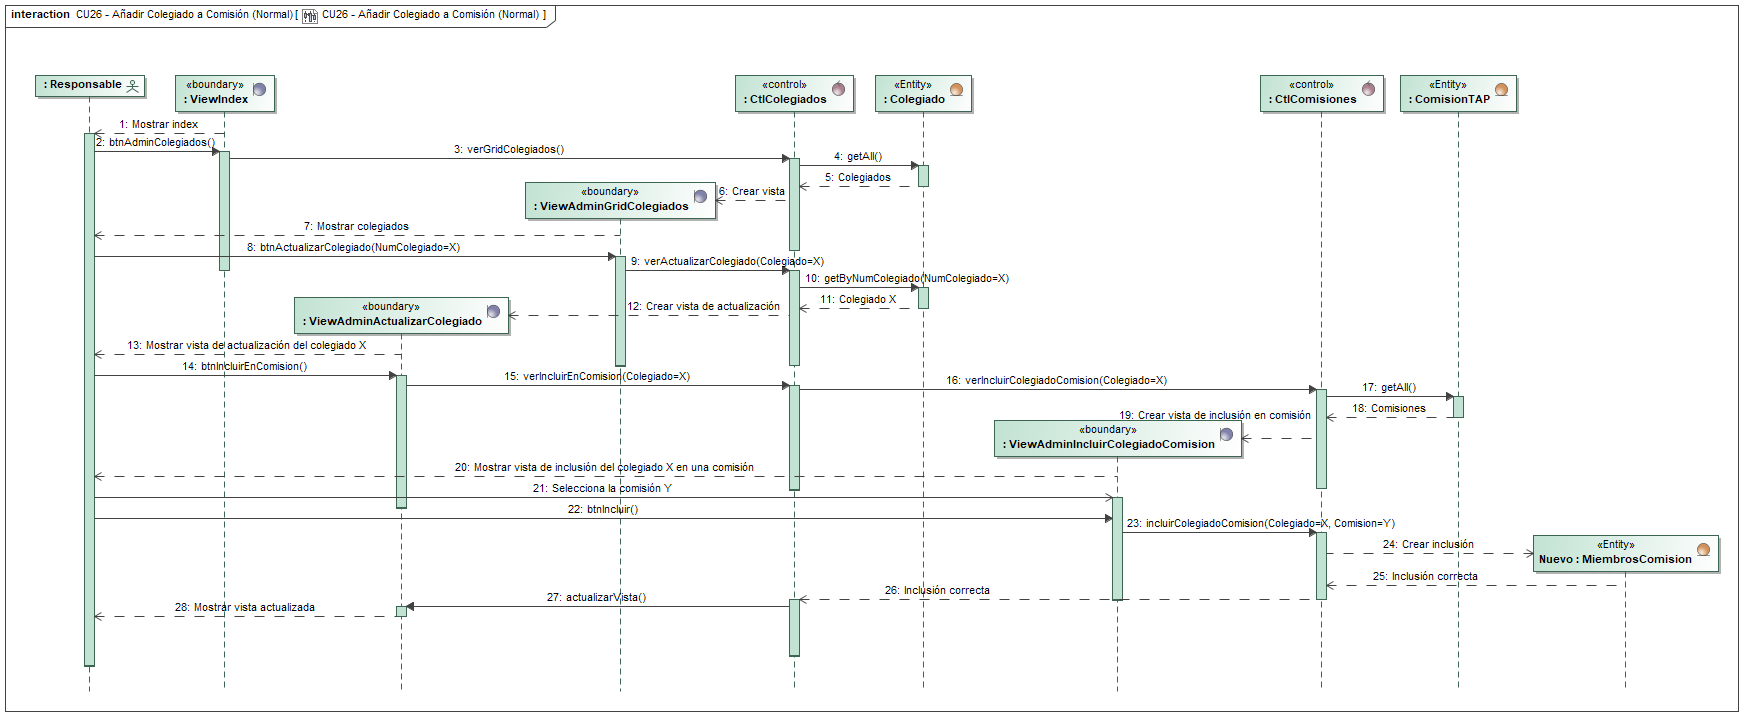
\includegraphics[width=150mm]{DiagramasSecuencia/CU26_Normal.png}
  \caption{Diagrama de Secuencia (Caso de Uso 26 - Flujo Normal)}
  \label{fig:Secuencia_CU26_Normal}
\end{figure}
\FloatBarrier

\begin{figure}[!htbp]
  \centering
  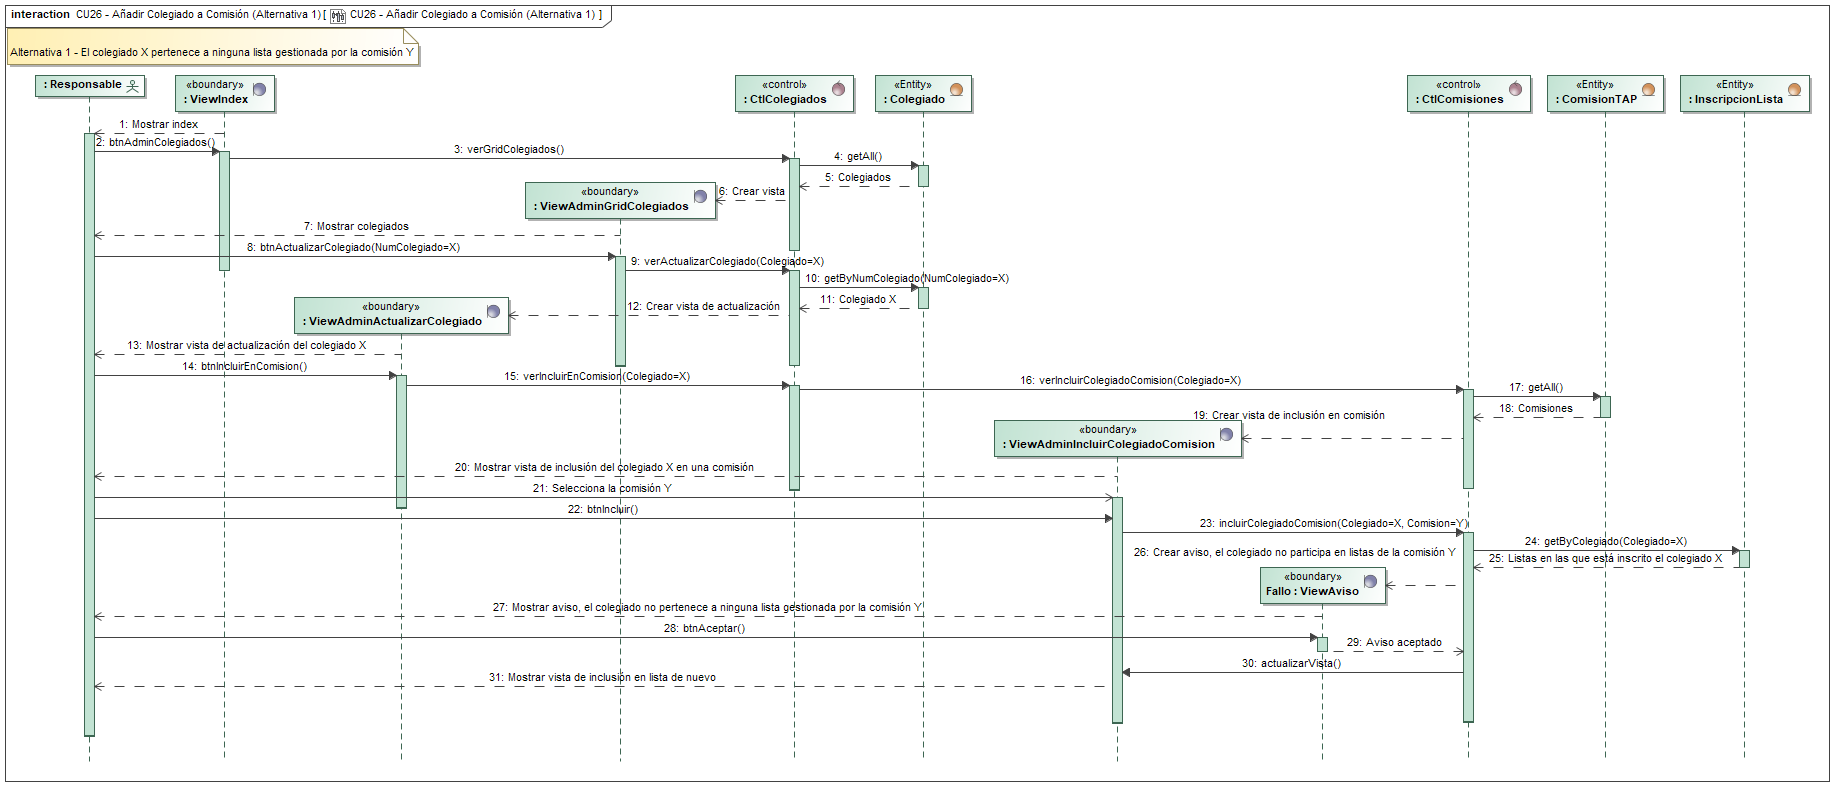
\includegraphics[width=150mm]{DiagramasSecuencia/CU26_Alt1.png}
  \caption{Diagrama de Secuencia (Caso de Uso 26 - Flujo Alternativo 1)}
  \label{fig:Secuencia_CU26_Alt1}
\end{figure}
\FloatBarrier

\addtocounter{figura}{1}
El caso de uso \textbf{\hyperref[tab:curExpulsarColegComisionTAP]{Expulsar Colegiado de la Comisión de TAP (CU27)}}, tiene únicamente un flujo de secuencia normal (\textbf{\hyperref[fig:Secuencia_CU27_Normal]{Figura \arabic{figura}}}).
\begin{figure}[!htbp]
  \centering
  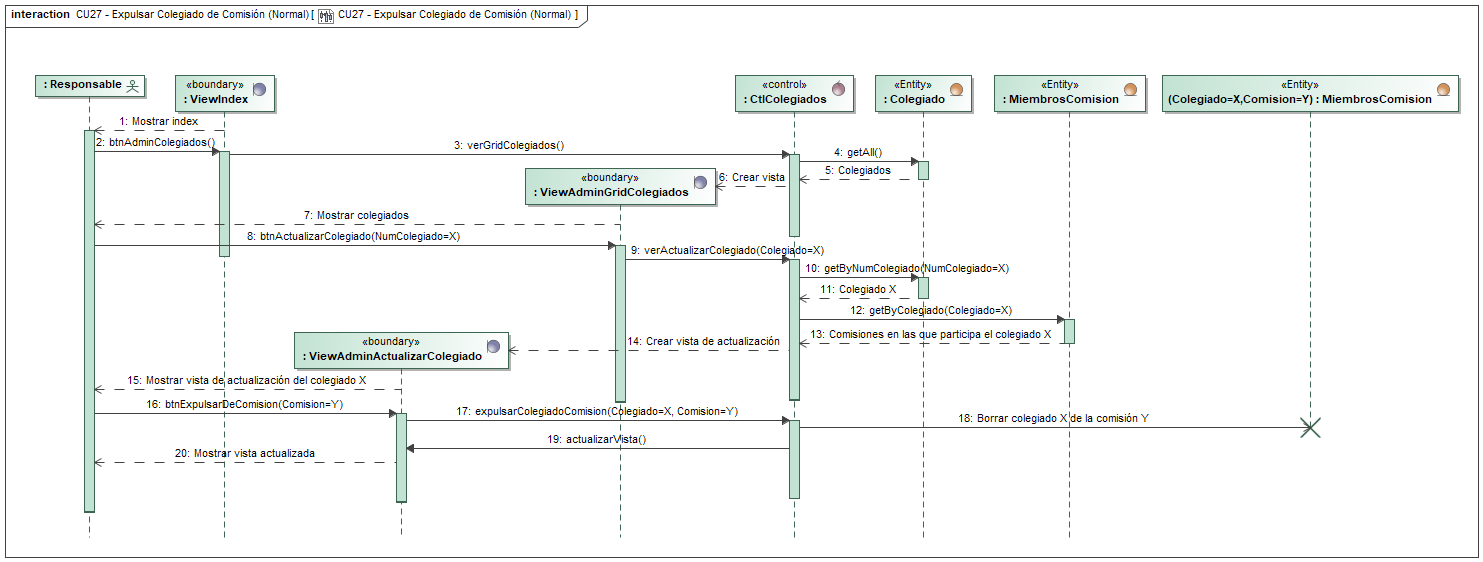
\includegraphics[width=150mm]{DiagramasSecuencia/CU27_Normal.png}
  \caption{Diagrama de Secuencia (Caso de Uso 27 - Flujo Normal)}
  \label{fig:Secuencia_CU27_Normal}
\end{figure}
\FloatBarrier

\addtocounter{figura}{1} \pagebreak
El caso de uso \textbf{\hyperref[tab:curAsignarPresidenciaComisionTAP]{Asignar Presidencia de Comisión de TAP (CU28)}}, tiene únicamente un flujo de secuencia normal (\textbf{\hyperref[fig:Secuencia_CU28_Normal]{Figura \arabic{figura}}}).
\begin{figure}[!htbp]
  \centering
  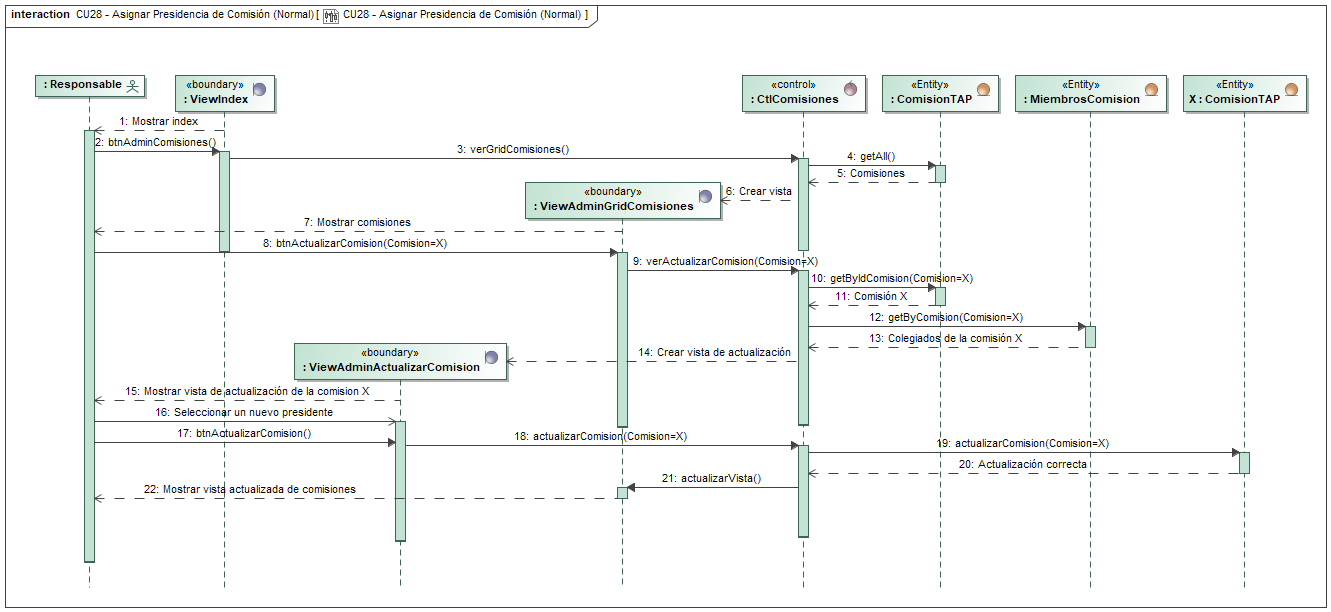
\includegraphics[width=150mm]{DiagramasSecuencia/CU28_Normal.png}
  \caption{Diagrama de Secuencia (Caso de Uso 28 - Flujo Normal)}
  \label{fig:Secuencia_CU28_Normal}
\end{figure}
\FloatBarrier

\addtocounter{figura}{1}
El caso de uso \textbf{\hyperref[tab:curInhabilitar]{Inhabilitar Colegiado (CU29)}}, tiene únicamente un flujo de secuencia normal (\textbf{\hyperref[fig:Secuencia_CU29_Normal]{Figura \arabic{figura}}}).
\begin{figure}[!htbp]
  \centering
  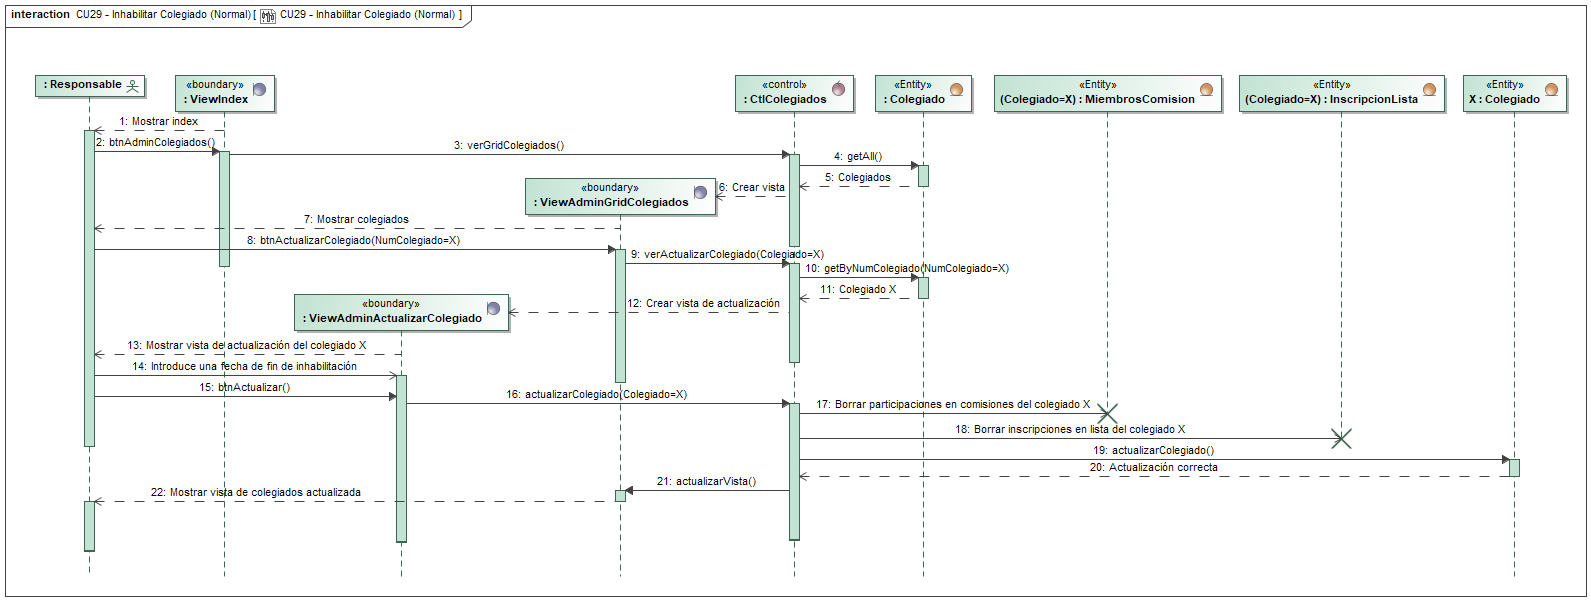
\includegraphics[width=150mm]{DiagramasSecuencia/CU29_Normal.png}
  \caption{Diagrama de Secuencia (Caso de Uso 29 - Flujo Normal)}
  \label{fig:Secuencia_CU29_Normal}
\end{figure}
\FloatBarrier

\addtocounter{figura}{1} \pagebreak
El caso de uso \textbf{\hyperref[tab:curConsultarProyectos]{Consultar Proyecto (CU30)}}, tiene únicamente un flujo de secuencia normal (\textbf{\hyperref[fig:Secuencia_CU30_Normal]{Figura \arabic{figura}}}).
\begin{figure}[!htbp]
  \centering
  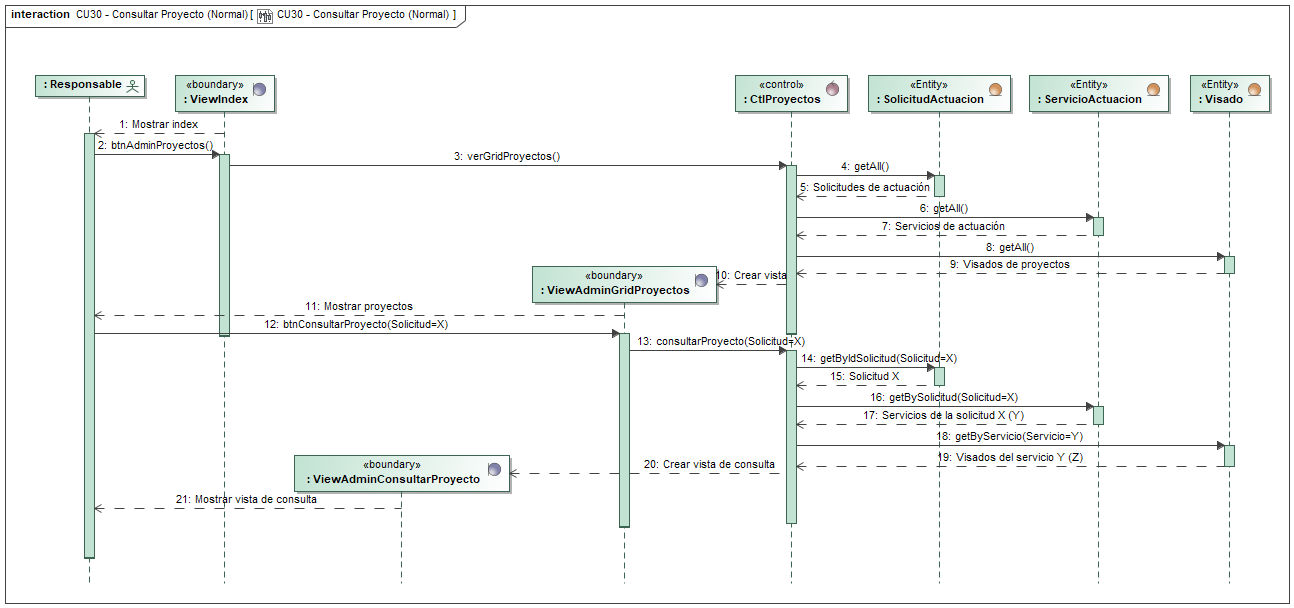
\includegraphics[width=150mm]{DiagramasSecuencia/CU30_Normal.png}
  \caption{Diagrama de Secuencia (Caso de Uso 30 - Flujo Normal)}
  \label{fig:Secuencia_CU30_Normal}
\end{figure}
\FloatBarrier

\addtocounter{figura}{1}
El caso de uso \textbf{\hyperref[tab:curActualizarProyecto]{Actualizar Estado del Proyecto (CU31)}}, tiene únicamente un flujo de secuencia normal (\textbf{\hyperref[fig:Secuencia_CU31_Normal]{Figura \arabic{figura}}}).
\begin{figure}[!htbp]
  \centering
  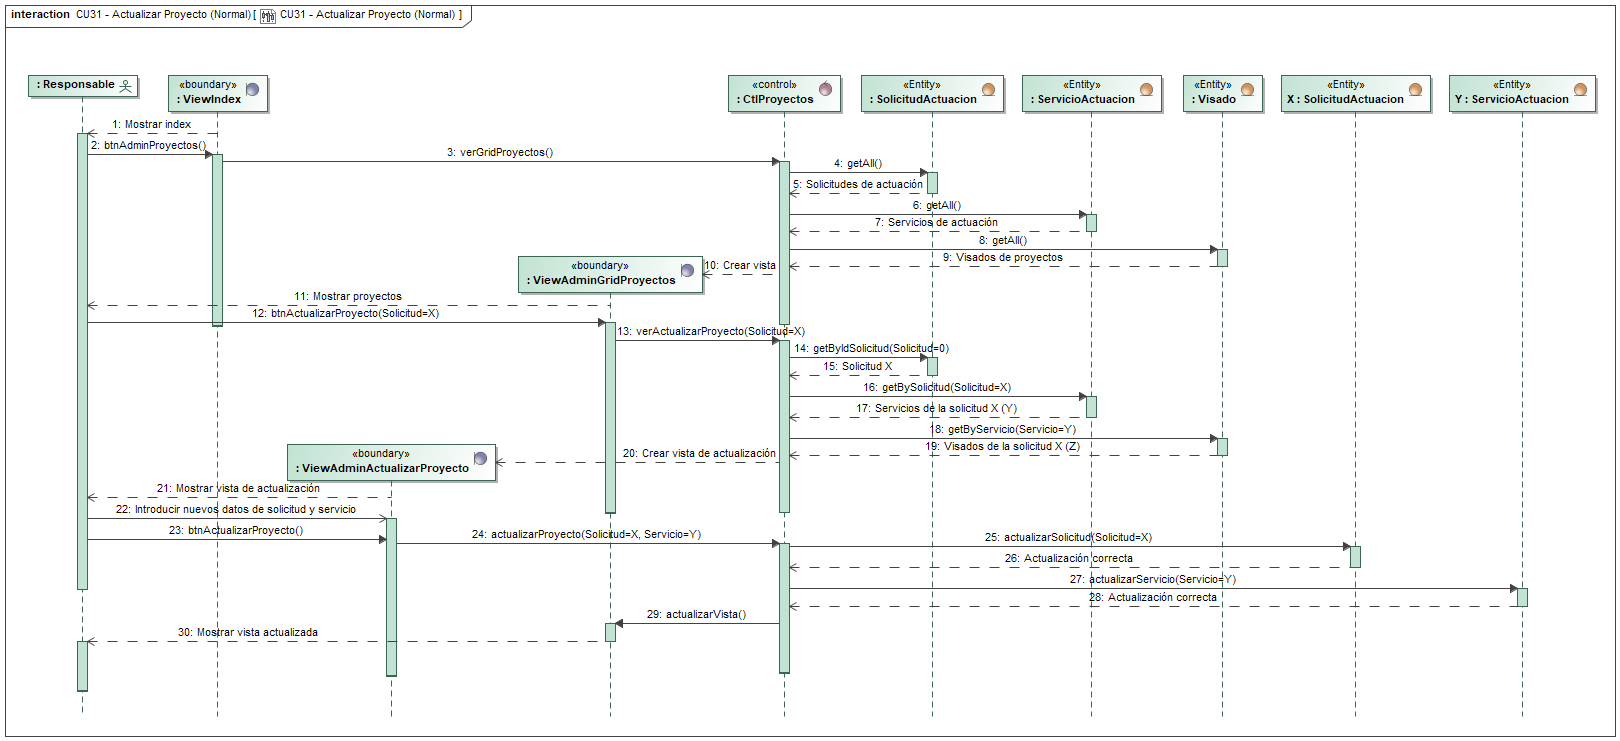
\includegraphics[width=150mm]{DiagramasSecuencia/CU31_Normal.png}
  \caption{Diagrama de Secuencia (Caso de Uso 31 - Flujo Normal)}
  \label{fig:Secuencia_CU31_Normal}
\end{figure}
\FloatBarrier

\addtocounter{figura}{1} \pagebreak
En \textbf{\hyperref[tab:curAsignarProfProyecto]{Añadir Profesional a Proyecto (CU32)}}, tenemos un flujo de secuencia normal (\textbf{\hyperref[fig:Secuencia_CU32_Normal]{Figura \arabic{figura}}}) \addtocounter{figura}{1} y uno alternativo si no hay ningún colegiado profesional disponible en la lista (\textbf{\hyperref[fig:Secuencia_CU32_Alt1]{Figura \arabic{figura}}}).
\begin{figure}[!htbp]
  \centering
  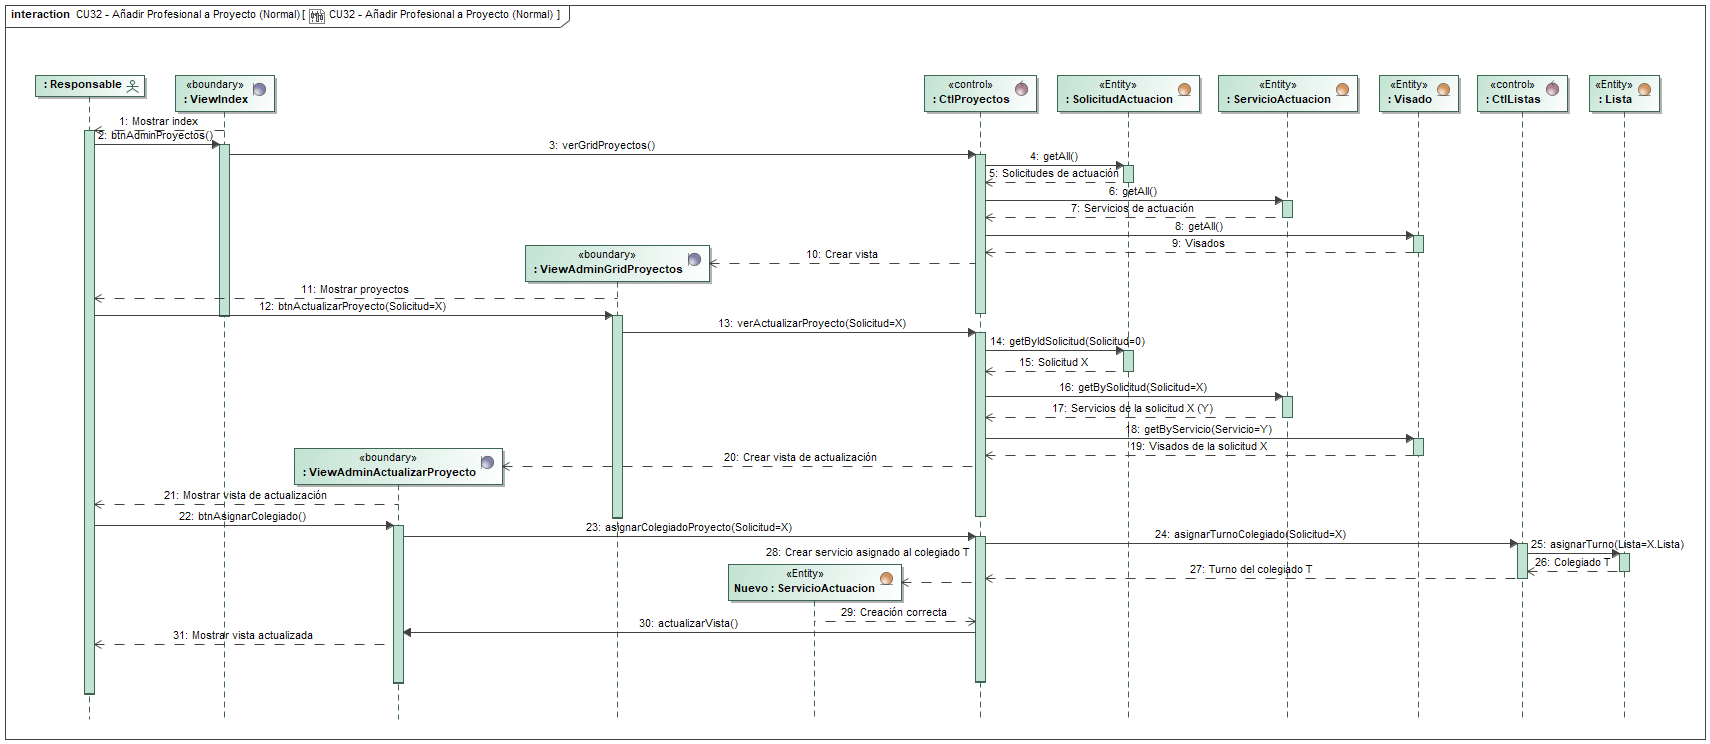
\includegraphics[width=150mm]{DiagramasSecuencia/CU32_Normal.png}
  \caption{Diagrama de Secuencia (Caso de Uso 32 - Flujo Normal)}
  \label{fig:Secuencia_CU32_Normal}
\end{figure}
\FloatBarrier

\begin{figure}[!htbp]
  \centering
  \includegraphics[width=150mm]{DiagramasSecuencia/CU32_Alt1.png}
  \caption{Diagrama de Secuencia (Caso de Uso 32 - Flujo Alternativo 1)}
  \label{fig:Secuencia_CU32_Alt1}
\end{figure}
\FloatBarrier

\addtocounter{figura}{1} \pagebreak
En \textbf{\hyperref[tab:curAsignarRevisorProyecto]{Añadir Revisor a Proyecto (CU33)}}, tenemos un flujo de secuencia normal (\textbf{\hyperref[fig:Secuencia_CU33_Normal]{Figura \arabic{figura}}}) \addtocounter{figura}{1} y uno alternativo si no hay ningún revisor disponible en la lista (\textbf{\hyperref[fig:Secuencia_CU33_Alt1]{Figura \arabic{figura}}}).
\begin{figure}[!htbp]
  \centering
  \includegraphics[width=150mm]{DiagramasSecuencia/CU33_Normal.png}
  \caption{Diagrama de Secuencia (Caso de Uso 33 - Flujo Normal)}
  \label{fig:Secuencia_CU33_Normal}
\end{figure}
\FloatBarrier

\begin{figure}[!htbp]
  \centering
  \includegraphics[width=150mm]{DiagramasSecuencia/CU33_Alt1.png}
  \caption{Diagrama de Secuencia (Caso de Uso 33 - Flujo Alternativo 1)}
  \label{fig:Secuencia_CU33_Alt1}
\end{figure}
\FloatBarrier

\addtocounter{figura}{1} \pagebreak
Por último, el caso de uso \textbf{\hyperref[tab:curAsignarTutela]{Asignar Tutelador a un Proyecto (CU34)}}, tiene únicamente un flujo de secuencia normal (\textbf{\hyperref[fig:Secuencia_CU34_Normal]{Figura \arabic{figura}}}).
\begin{figure}[!htbp]
  \centering
  \includegraphics[width=150mm]{DiagramasSecuencia/CU34_Normal.png}
  \caption{Diagrama de Secuencia (Caso de Uso 34 - Flujo Normal)}
  \label{fig:Secuencia_CU34_Normal}
\end{figure}
\FloatBarrier
